\documentclass[14pt, a4paper]{extarticle}
%, draft
\usepackage[utf8]{inputenc}
\usepackage{ucs}
\usepackage[russian]{babel} 
\usepackage[T2A]{fontenc}
\usepackage[pdftex]{graphicx}
\usepackage{amstext}
\usepackage{amsmath}
\usepackage{cmap} % чтобы был поиск по pdf
\usepackage{textcomp}
\usepackage{multicol}
\usepackage{hyperref}
\usepackage{setspace}
\usepackage[usenames,dvipsnames]{color} % для source-highlight
\usepackage{indentfirst}
\usepackage{clrscode}
\usepackage{longtable}
\usepackage{float} % \begin{figure}[H]

% меняем размеры страницы
\usepackage{geometry}
\geometry{left=2.5cm}
\geometry{right=2.0cm}
\geometry{top=2.0cm}
\geometry{bottom=2.5cm}

\newcommand{\normalize}{\mathrm{normalize}}

% отступ при наборе формул в блоке multline
\multlinegap=2cm

% будем считать что переполнения не было, если строка вышла за границу не более чем 0.01pt
\hfuzz=0.01pt

% разрешаю увеличить расстояние между словами не больше чем на 11pt, что бы не было переполнения
\emergencystretch=11pt

% изменение межстрочного интервала
\def\heightline{1.3}
\linespread{\heightline} % 1.3 - это полуторный

%%%%%%%%%%%%%%%%%%%%%%%%%%%%%%%%%%%%%%%%%%%%%%%%
%%% добавляем точки в Оглавление

\renewcommand{\thesection}{\arabic{section}.} 
\renewcommand{\thesubsection}{\arabic{section}.\arabic{subsection}.} 
\renewcommand{\thesubsubsection}{\arabic{section}.\arabic{subsection}.\arabic{subsubsection}.} 

%%%%%%%%%%%%%%%%%%%%%%%%%%%%%%%%%%%%%%%%%%%%%%%%

% определим новые команды
\def\VEC#1#2#3{\left( \begin{array}{c} #1 \\ #2 \\ #3 \end{array} \right) }
\def\VECXYZ#1{\left( \begin{array}{c} x_#1 \\ y_#1 \\ z_#1 \end{array} \right) }

\newcommand{\HRule}{\noindent\rule{\linewidth}{0.45mm}}

\newcounter{sourcecode}
\setcounter{sourcecode}{0}
\newcommand*{\cppsource}[2]{\refstepcounter{sourcecode} \par{\HRule \small \tt \bf \noindent \ Листинг \arabic{sourcecode}. {\rm \small #2} \vspace{0.25cm}}%
\input{#1} \HRule}

\makeindex

\begin{document}

\begin{titlepage}
\begin{center}
{Федеральное агентство по образованию Российской Федерации\\ 
Государственное образовательное учреждение \\ 
высшего профессионального образования \\ 
Нижегородский государственный университет им. Н.И. Лобачевского\\
Факультет вычислительной математики и кибернетики\\
Кафедра математического обеспечения ЭВМ\\
\vspace{2em}
Дипломная работа\\
}
{\bf \Large	\textsf{ Трассировка лучей в реальном времени на~x64~архитектуре \\ } }
\end{center}
\vspace{1em}
\begin{multicols}{2}
\noindent 
Работа допущена к защите \\
Заведующий кафедрой МО ЭВМ \\
д.ф.--м.н., проф. \\

\vspace*{1em}
{ \noindent
\hspace*{1.5cm}\hbox to 0cm{\raisebox{-1em}{\small Подпись}}\hspace{-1.5cm}{\hrulefill\ Стронгин Р. Г. }
}

\vspace*{1.0em}
{ \noindent
\hbox to 0cm{\raisebox{0.25em}{<<\ \ \ \ \ \  >>}}{\hrulefill\ 2011 г. }
}
\vbox to 5 cm{\ }
Исполнитель: \\
студент 2 курса магистратуры \\
факультета ВМК группы 86М1 \\

\vspace*{1em}
{ \noindent
\hspace*{1.5cm}\hbox to 0cm{\raisebox{-1em}{\small Подпись}}\hspace{-1.5cm}{\hrulefill\ Морозов А. С. }
}

\vspace*{1em}
{ \noindent
\hbox to 0cm{\raisebox{0.25em}{<<\ \ \ \ \ \  >>}}{\hrulefill\ 2011 г. }
}
\\
Научный руководитель: д. т. н., \\
профессор кафедры МО ЭВМ \\

\vspace*{1em}
{ \noindent
\hspace*{1.5cm}\hbox to 0cm{\raisebox{-1em}{\small Подпись}}\hspace{-1.5cm}{\hrulefill\ Турлапов В. Е. }
}

\vspace*{1em}
{ \noindent
\hbox to 0cm{\raisebox{0.25em}{<<\ \ \ \ \ \  >>}}{\hrulefill\ 2011 г. }
}
\end{multicols}

\vfill 
\begin{center} 
{\rm Нижний Новгород \\ 2011 г.} 
\end {center} 
\end{titlepage} 

\tableofcontents

\newpage
\section*{Введение}
\addcontentsline{toc}{section}{Введение} 
В киноиндустрии к современной компьютерной графике предъявляются серьезные требования физически корректного моделирования освещения сцен. Каждая из них состоит из множества примитивов с различными характеристиками, которые по разному взаимодействуют со светом. Даже малейшие неточности, могут отбросить художественный или анимационный фильм в рубрику любительского кино, и при этом не принести ожидаемой прибыли. Особенные требования предъявляются именно к художественному фильму, т. к. используемые спецэффекты должны выглядеть настолько реалистично, что бы зритель не смог различить, где настоящий актер, а где рисованный двойник, выполняющий невероятные трюки. Используя только физически правильные модели и алгоритмы можно обеспечить растущую потребность в более реалистичной трехмерной графике.

   С каждым новым фильмом, каждый из нас видит прогресс в компьютерной графике. Картинка становится все красочнее и правдоподобнее, но это все не дается просто так. Естественно, платить за это приходится высокой вычислительной трудоемкостью расчетов. Несомненно, что с каждым годом производительность вычислительной техники растет, но она сразу ''расходуются'' на новые спецэффекты. Существует наблюдение, которое гласит, что время расчета одного кадра не изменяется. Среднее время расчета полного фильма 15 лет назад занимал около 10-12 месяцев, так и сегодня, тратят столько же времени, хотя при этом, надо заметить, что производительность современных компьютеров в сотни раз превышает производительность компьютеров того времени. С развитием вычислительной техники растут требования к самому изображению. Если несколько лет назад картинка с разрешением 1024х768 считалась излишеством в компьютерной графики, то уже сейчас это слишком мало и все считают де факто FullHD\footnote{ \index{FullHD}FullHD -- это разрешение экрана 1920х1080 пикселей}. В последний год компьютерная индустрия, дабы не потерять зрителя, начала использовать новые технологии — 3D, которая требует еще большей вычислительной мощности. 

   Именно за последние несколько лет компьютеры стали по настоящему параллельными. Появились многоядерные процессоры. И именно по этому, что 15 лет назад было трудоемкой задачей рендеринга, то сейчас это можно получить почти в реальном времени при том же качестве результата.

\newpage 
\section{Постановка задачи}
Главной целью данной работы является исследование и реализация алгоритма трассировки лучей на архитектуре x64. Для решения главной задачи, требуется решить ряд следующих подзадач:
\begin{itemize}
	\item Реализовать высокопроизводительный алгоритм трассировки лучей на центральном процессоре
	\item Реализация и исследование оптимизированной версии с использованием векторных расширений архитектуры x64
	\item Реализация и исследование специализированного класса векторов для алгоритма трассировки лучей основанного на технологии шаблонных выражений, с применением векторных оптимизаций -- \index{SIMD}SIMD\footnote{ Single Instruction, Multiple Data — Одна Инструкция, Много Данных } инструкции, что должно дать хорошую скорость работы приложения без потери качества восприятия кода
	\item Реализация параллельной версии алгоритма трассировки лучей с использованием OpenMP, TBB
	\item Сравнение параллельной версии алгоритма трассировки лучей с использованием библиотеки TBB и OpenMP на многоядерном процессоре с технологией \index{HT}HT\footnote{HT - Hyper-Threading или Гиперпоточность }
	\item Алгоритмическая оптимизация : реализация ускоряющей структуры
	\item Сравнение реализации алгоритма с использованием ускоряющей структуры и без нее
\end{itemize}
   В качестве основного языка программирования выбирается язык С++, а для отображения результатов — кроссплатформенная библиотека SDL. 
   
\newpage 
\section{Архитектура центрального процессора}

Для того, что бы ответить на вопрос, почему же была выбрана архитектура x86-64 для написание столь сложного и трудоемкого приложения, необходимо рассмотреть её основные особенности.

Одни из базовых понятий для производительности процессора:
\begin{itemize}
\item Количества тактов процессора затрачиваемое на обработку инструкции пока она проходит все стадии в процессоре(Latency)
\item Количества тактов процессора необходимое на принятие инструкции на обработку(Throughput)
\end{itemize}

\noindent
В процессоре используется различный уровень параллелизма:
\begin{itemize}
\item Суперскалярность — имеется несколько исполнительных блоков
\item SIMD(Single Instruction, Multiple Data) – параллельная обработка по данным
\item Конвеерность
\item SMT – Simultaneous Multi-Threading – одновременное использование ресурсов несколькими процессами, конвеер использоется лучше, вычислительные блоки не простаивают
\item SMP – Symmetric Multi-Processing (многоядерные процессоры)
\end{itemize}


\subsection{Архитектура процессора Pentium 4}
Intel Pentium 4 -- это одноядерный x86 - совместимый микропроцессор компании Intel, представленный 20 ноября 2000 года.

В основе архитектуры любого процессора лежат несколько обязательных конструктивных элементов: кэш команд и данных, предпроцессор и блоки исполнения команд.

Процесс обработки данных состоит из нескольких характерных этапов. Сначала инструкции и данные забираются из кэша, который разделен на кэш данных и кэш инструкций, -- эта процедура называется выборкой. Затем выбранные из кэша инструкции декодируются в понятные для данного процессора примитивы -- микроинструкции (uops), и называется данная процедура декодированием. Далее декодированные команды поступают на исполнительные блоки процессора, где и выполняются, а результат записывается в оперативную память.

Процессы выборки инструкций из кэша, их декодирование и продвижение к исполнительным блокам осуществляются в предпроцессоре, а процесс выполнения декодированных команд — в блоке исполнения команд. Таким образом, даже в самом простейшем случае команда проходит как минимум четыре стадии обработки:
\begin{itemize}
\item выборка из кэша;
\item декодирование;
\item выполнение;
\item запись результатов.
\end{itemize}

Указанные стадии принято называть конвейером обработки команд. В простейшем случае конвейер является четырехступенчатым, и каждую из этих ступеней команда должна проходить ровно за один такт. Для четырехступенчатого конвейера на выполнение одной команды соответственно отводится ровно четыре такта.
В реальных процессорах конвейер обработки команд может быть более сложным и включать большее количество ступеней. Собственно говоря, отличительной особенностью процессоров семейства Intel Pentium 4 и является их беспримерно длинный конвейер. Так, в процессорах на ядре Northwood длина конвейера составляла 20 ступеней, а в новом процессоре Prescott она увеличена до 31 ступени. Причина увеличения длины конвейера заключается в том, что поскольку многие команды являются довольно сложными и не могут быть выполнены за один такт процессора, особенно при высоких тактовых частотах, то каждая из четырех стадий обработки команд (выборка, декодирование, выполнение, запись) должна состоять из нескольких ступеней конвейера. Кроме того, в конвейер преднамеренно вставляются так называемые пустые ступени (Drive), на которых не происходит обработка инструкции.

Эти пустые (или передаточные) ступени необходимы для того, чтобы при высоких тактовых частотах сигнал успевал во время одного такта распространится от одного исполнительного блока к другому. Напомним, что при частотах свыше 3 ГГц время одного такта составляет менее 3 нс. За столь короткий промежуток времени свет в вакууме успевает пройти расстояние менее 1 см, а поскольку скорость распространения сигналов в кристалле существенно ниже скорости света, то при высоких тактовых частотах неизбежно приходится вводить пустые ступени конвейера для передачи сигнала.

Всякий процессор в конечном счете должен быть сконструирован таким образом, чтобы за минимальное время выполнять максимальное количество инструкций. Именно количество выполняемых за единицу времени инструкций и определяет производительность процессора.

Существует два принципиально различных способа повышения производительности процессора (не считая, конечно, увеличения тактовой частоты). Суть первого состоит в том, чтобы увеличивать количество исполнительных блоков — таким образом реализуется множество параллельных коротких конвейеров. Данный подход позволяет в полной мере реализовать параллелизм на уровне инструкций (Instruction-Level Parallelism, ILP), когда несколько инструкций выполняются одновременно в различных исполнительных блоках процессора. Количество ступеней конвейера здесь невелико, поэтому инструкции выполняются за небольшое количество циклов.

Для реализации параллелизма на уровне инструкций необходимо, чтобы поступающие на исполнительные блоки команды можно было выполнять параллельно. Однако если, к примеру, для выполнения следующей по порядку инструкции требуется знать результат выполнения предыдущей инструкции (подобные инструкции называются взаимозависимыми), то в этом случае параллельное выполнение невозможно. Поэтому препроцессор прежде всего проверяет взаимозависимость команд и переупорядочивает их — не в порядке поступления (Оut of Оrder), а так, чтобы их можно было выполнять параллельно. На последних ступенях конвейера инструкции выстраиваются в исходном порядке.

При коротком конвейере на каждой ступени процессор способен выполнять большее количество работы, однако на прохождение инструкции через каждую ступень конвейера здесь затрачивается больше времени, что ограничивает повышение тактовой частоты процессора. В этой ситуации увеличение числа команд, выполняемых за единицу времени, достигается за счет распараллеливания инструкций и наращивания исполнительных блоков процессора.

При использовании длинного конвейера возможно увеличение тактовой частоты процессора, то есть сам конвейер оказывается более быстрым. Применение длинных конвейеров с высокими тактовыми частотами процессора — это второй способ увеличения производительности процессора, и именно такая идеология длинного конвейера заложена в архитектуре процессора Intel Pentium 4. При использовании длинного конвейера на стадии исполнения инструкций задействуется меньшее количество исполнительных блоков, но каждый из них обладает длинным и соответственно быстрым конвейером. Это означает, что каждый блок исполнения (Execution Unit) имеет больше доступных для выполнения тактов и способен одновременно выполнять довольно много инструкций.

\begin{figure}
\centering
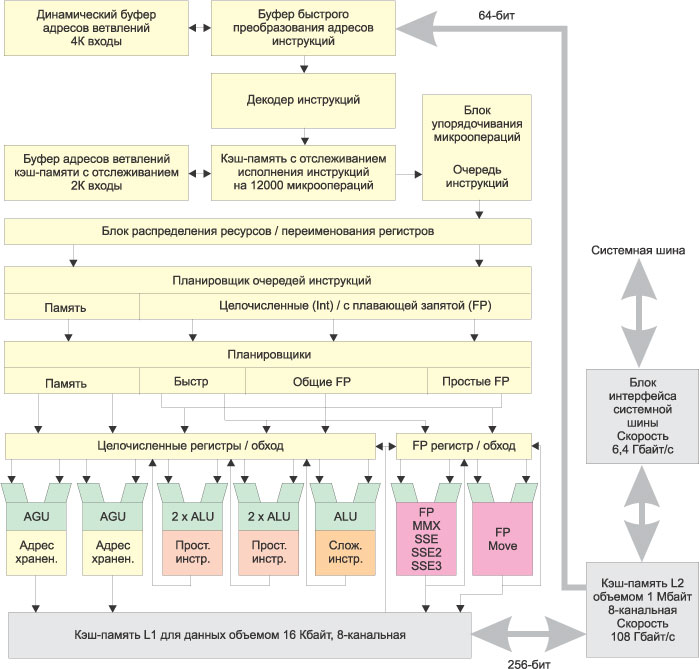
\includegraphics[width=\textwidth]{imgs/ap4.jpg}
\caption{Архитектура процессора Pentium 4}\label{fig:arch_p4}
\end{figure}

Этот метод имеет, однако, свои подводные камни. Дело в том, что в случае длинного конвейера предпроцессору необходимо обеспечивать ему соответствующую загрузку. Для этого предпроцессор должен обладать довольно большим буфером, способным вмещать достаточное количество инструкций. Если же в кэше отсутствует инструкция или данные для конвейера, то образуются так называемые конвейерные пузырьки (Рipeline Вubbles), которые проходят все ступени конвейера, но ни на одной из них не производятся никакие действия. Наличие Рipeline Вubbles негативно отражается на производительности процессора, поскольку ресурсы процессора просто-напросто простаивают. Избежать возникновения нежелательных простоев в процессорах позволяют различные хитроумные алгоритмы, например Hyper-Threading.
Как уже отмечалось выше, новый процессор Prescott имеет необычайно длинный конвейер — 31 ступень, что на 11 степеней больше, чем в процессоре Northwood. При этом архитектура Intel NetBurst, заложенная в процессоре, не претерпела существенных изменений. Структурная схема процессора изображена на рис \ref{fig:arch_p4}.


При работе процессора инструкции выбираются из кэша L2 и декодируются. Кэш L2 процессоров семейства Pentium 4 под названием Advanced Transfer Cache, имеет 256-битную шину, работающую на частоте ядра, и усовершенствованную схему передачи данных, кэш обеспечивает высочайшую пропускную способность, столь важную для потоковых процессов обработки.

Для выборки команд из кэша L2 и их последующего декодирования в микрооперации отводится несколько начальных ступеней конвейера. Соответственно при выполнении фрагмента программного кода для декодирования команд будет использовано несколько процессорных тактов. Однако во многих современных (прежде всего мультимедийных) приложениях один и тот же фрагмент кода может повторяться многократно, и было бы нерационально тратить процессорные такты на повторную выборку, транслирование и декодирование. Выгоднее хранить уже готовые к исполнению микроинструкции в специальном кэше L1, где из них формируются мини-программы, называемые отслеживаниями (Тraces). Каждая такая программа может содержать до 6 декодированных инструкций uops. Мини-программы формируются из инструкций, которые выполняются последовательно (именно поэтому они и называются отслеживаниями). При этом в самом программном коде указанные инструкции могут не следовать друг за другом, то есть реализуется внеочередное выполнение инструкций (Оut-of-Оrder). При попадании в кэш L1 происходит внеочередное выполнение команд; при этом значительно экономятся ресурсы процессора, так как по своей сути внеочередное выполнение команд подразумевает устранение первых ступеней конвейера, фактическая длина которого в этом случае составляет уже 31 ступень. В кэше с отслеживанием может храниться до 12 тыс. декодированных микрокоманд.

Режим работы процессора при внеочередном выполнении команд (то есть когда происходит попадание в Trace Cache и используются уже декодированные команды) является естественным для процессора Intel Pentium 4. Поэтому, говоря о длине конвейера в 31 ступень, мы имеем в виду длину основного конвейера — без учета первых ступеней, которые используются при необходимости выборки команд, их трансляции, декодирования и сохранения в Trace Cache полученных микрокоманд.

Чтобы обеспечить высокий процент попаданий в кэш L1 с отслеживаниями (Trace Cache) и построение в нем мини-программ, используется специальный блок предсказания ветвлений (Branch Targets Buffers, BTB и Instruction Translation Look-aside Buffers, I-TLB). Этот блок позволяет модифицировать мини-программы, основываясь на спекулятивном предсказании. Так, если в программном коде имеется точка ветвления, то блок предсказаний может предположить дальнейший ход программы вдоль одной из возможных ветвей и с учетом этого спекулятивного предсказания построить мини-программу.

Рассмотрим теперь процесс продвижения микроинструкций по основному конвейеру, то когда процессор работает в режиме внеочередного выполнения инструкций. В течение первых двух тактов в Trace Cache передается указатель на следующие выполняемые инструкции — это две первые ступени конвейера, называемые Trace Cache next instruction pointer. После получения указателя в течение двух тактов происходит выборка инструкций из кэша (Trace Cache Fetch) — это две следующие ступени конвейера. Затем выбранные инструкции должны быть отосланы на внеочередное выполнение. Для того чтобы обеспечить продвижение выбранных инструкций по процессору, используется еще одна дополнительная, или передаточная, ступень конвейера (Drive).

На следующих ступенях конвейера, которые называются Allocate \& Rename, происходят переименование и распределение дополнительных регистров процессора. В процессоре Intel Pentium 4 содержится 128 дополнительных регистров, которые не определены архитектурой набора команд. Переименование регистров позволяет добиться их бесконфликтного существования.

Далее формируются две очереди (Queue) микрокоманд: очередь микрокоманд памяти (Memory uop Queue) и очередь арифметических микрокоманд (Integer/Floating Point uop Queue).

На следующих ступенях конвейера происходит планирование и распределение (Schedule) микрокоманд. Планировщик (Scheduler) — это своего рода сердце ядра процессора  — выполняет две основные функции: переупорядочивание микрокоманд и распределение их по функциональным устройствам. Суть переупорядочивания микрокоманд заключается в том, что планировщик определяет, какую из них уже можно выполнять и в соответствии с их готовностью меняет порядок следования. Распределение микрокоманд происходит по четырем функциональным устройствам, то есть формируются четыре очереди. Первые две из них предназначены для устройств памяти (Load/Store Unit) и формируются планировщиком Memory Scheduler из очереди памяти Mem uop Queue. Микрокоманды из очереди арифметических микрокоманд (Integer/Floating Point uop Queue) также распределяются в очереди соответствующих функциональных устройств, для чего предназначено три планировщика: Fast ALU Scheduler, Slow ALU/General FPU Scheduler и Simple FP Scheduler.

Fast ALU Scheduler — это распределитель простых целочисленных операций, который собирает простейшие микроинструкции для работы с целыми числами, чтобы затем послать их на исполнительный блок ALU, работающий на двойной скорости. В процессоре Pentium 4 имеются два исполнительных блока ALU, работающих на удвоенной скорости. К примеру, если тактовая частота процессора составляет 3,2 ГГц, то эти два устройства ALU работают с частотой 6,4 ГГц и в параллельном режиме способны выполнять четыре целочисленные операции за один такт. Такие блоки ALU получили название Rapid Execution Engine (блоки быстрого исполнения). Отметим, что в процессоре Prescott в один из быстрых блоков ALU добавлен блок Shifter/Rotator, исполняющий инструкции типа сдвига и вращения. Благодаря этому такие инструкции теперь исполняются гораздо быстрее, поскольку в предыдущих реализациях Pentium 4 сдвиг и вращение трактовались как сложные инструкции и выполнялись на медленном ALU.

\subsection{Архитектура процессора Nehalem}

Для того, что бы понять как эволюционировал центральный процессор необходимо рассмотреть, для сравнения, современный процессор.

Intel Nehalem -- микропроцессорная архитектура компании Intel, представленная в 4 квартале 2008 года. 

x86-64 (также x64/AMD64/Intel64/EM64T) -- это  64-битная аппаратная платформа (чипсет, архитектура микропроцессора и команд), разработанная компанией AMD для выполнения 64-разрядных приложений.
Это расширение архитектуры x86 с полной обратной совместимостью.

Основные особенности архитектуры x64:
\begin{itemize}
\item 16 целочисленных 64-битных регистра общего назначения (RAX, RBX, RCX, RDX, RBP, RSI, RDI, RSP, R8 — R15);
\item 8 80-битных регистров с плавающей точкой (ST0 — ST7);
\item 8 64-битных регистров Multimedia Extensions (MM0 — MM7, имеют общее пространство с регистрами ST0 — ST7);
\item 16 128-битных регистров SSE (XMM0 — XMM15);
\item 64-битный указатель RIP и 64-битный регистр флагов RFLAGS.
\end{itemize}

\begin{figure}
\centering
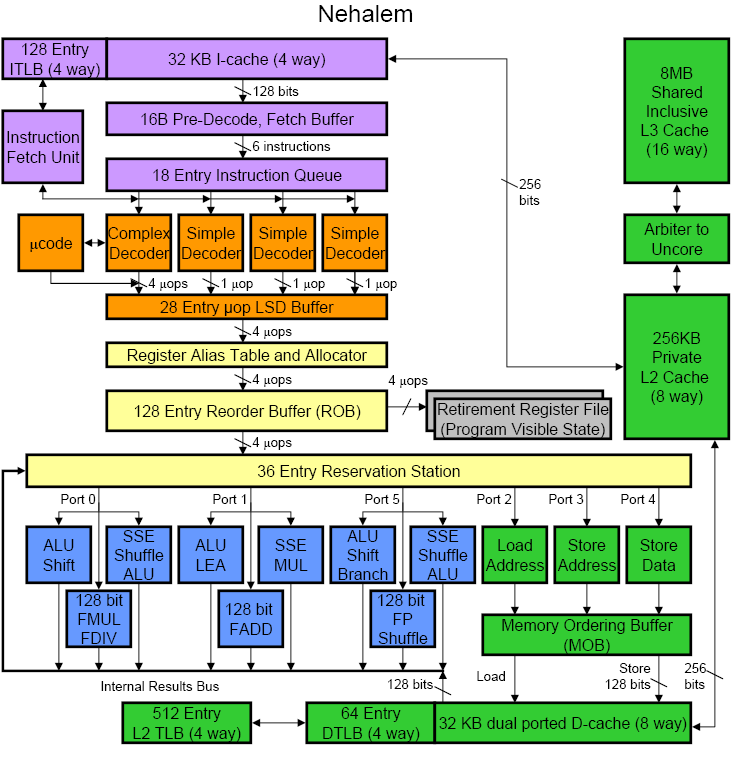
\includegraphics[width=\textwidth]{imgs/nehalem.png}
\caption{Архитектура процессора Nehalem}\label{fig:arch_nehalem}
\end{figure}

По сравнению с серией Pentium процессоры Nehalem продвинулись далеко вперед по интенсивному пути, а именно не увеличивая количества вычислительных блоков (на ядро). С увеличением количество ядер на кристалле возрастала и производительность. Достичь этого удалось благодаря определению оптимальной длины конвейера, а также за счет увеличенных буферов по переупорядочиванию и буфера декодированных инструкций, ко всему прочему увеличился процент предсказания ветвлений и за счет подрастания тактовых частот. Увеличенный кэш второго третьего уровня позволил меньше обращаться к оперативной памяти, в результате чего скорость программ значительно увеличилась. Еще одним из не мало важных факторов, который внес существенную часть производительности в процессор это технология компании Intel называемая Hyper-threading. Проблема заключалось в том, что процессор выполняя программы даже после переупорядочиваний инструкций все равно простаивал по большей части. Это связано с тем, что данные в программе сильно зависимы. Данная технология помогла решить данную проблему, тем самым еще больше повысив эффективность использования вычислительных блоков(рис.~\ref{fig:smt}). Суть технологии в том, что одно физическое ядро одновременно исполняет 2 потока данных.

\begin{figure}
\centering
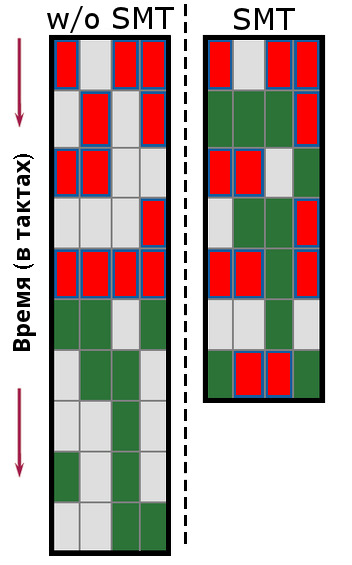
\includegraphics[scale=0.65]{imgs/smt.png}
\caption[Технология Simultaneous MultiThreading]{Технология Simultaneous MultiThreading, улучшенная технология Intel Hyper-Threading}\label{fig:smt}
\end{figure}

\begin{figure}
\centering
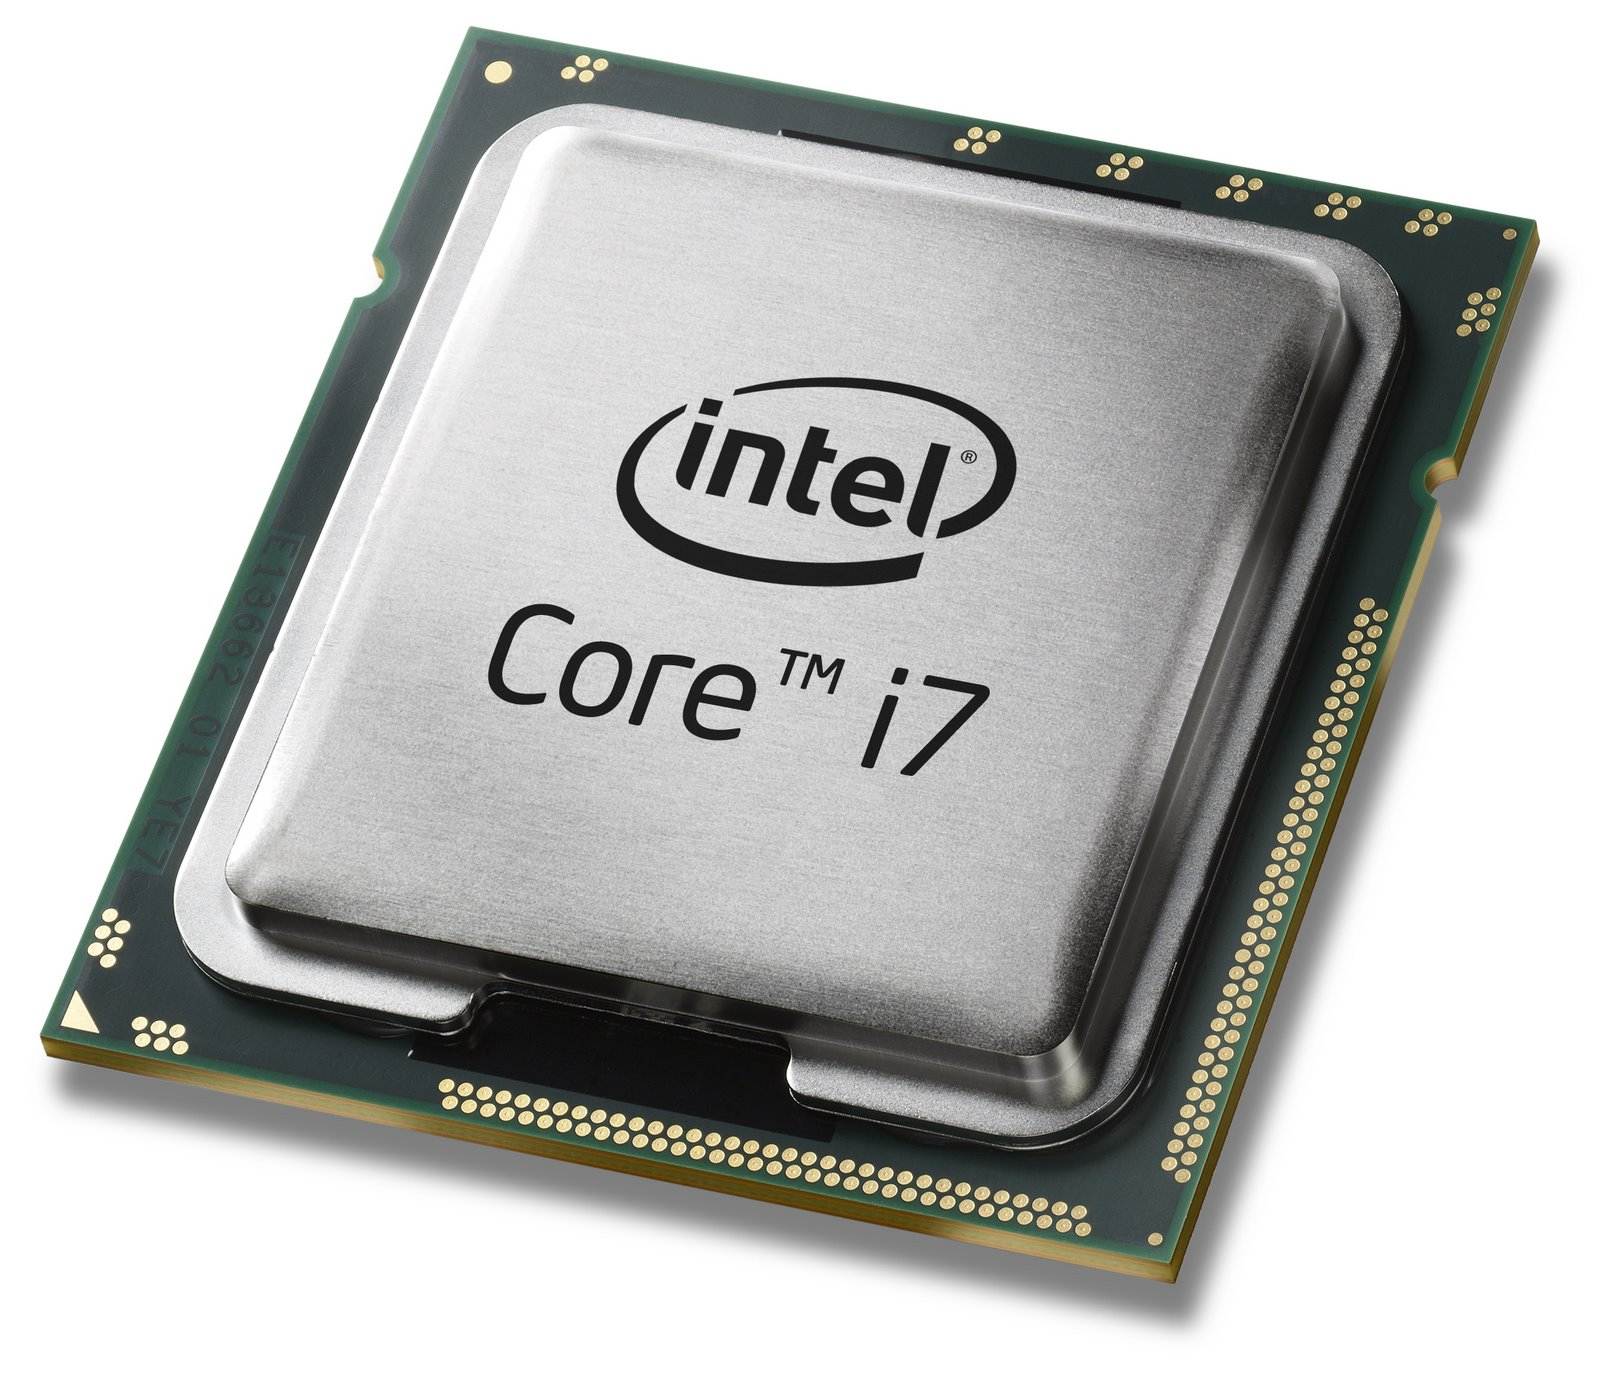
\includegraphics[width=0.35\textwidth]{imgs/corei7.jpg}
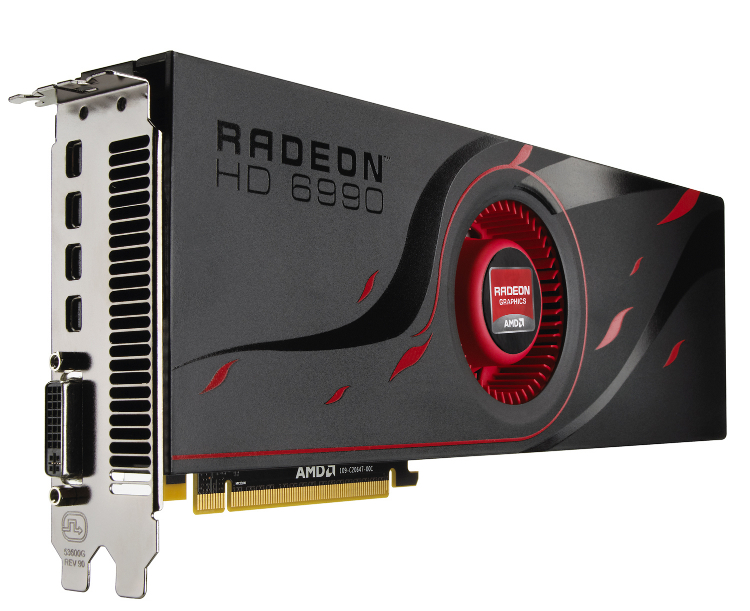
\includegraphics[width=0.45\textwidth]{imgs/radeon6990.jpg}
\caption[Самый быстрый CPU и GPU]{Самый быстрый центральный процессор Intel Core i7 990X и самая быстрая видеокарта AMD Radeon HD 6990 на Q2 2011}\label{fig:imgs_corei7}
\end{figure}

Центральный процессор в первую очередь ориентировался на быстрое исполнение кода при имеющихся скромных ресурсах, в отличие от GPU, у которых изначально закладывалась мысль о параллельной обработке данных, поэтому у графической карты производительность каждого ядра очень мала, но большое количество ядер позволяют графическим ускорителям иметь большую производительность. Для примера, можно посмотреть на производительность 6 ядерного процессора Intel Core i7 990X Extreme Edition~\cite{perf_core_i7}, у которого пиковая производительность равна 109 Gflops и графический ускоритель AMD Radeon HD 6990~\cite{perf_radeon6990}, содержащий 3072 ядер, с пиковой производительностью равной 5100 Gflops. При перерасчете на ядро получаем, что центральный процессор имеет 18,16 Gflops/Core, а графический ускоритель всего 1,66 Gflops/Core. Таким образом получаем, что одно ядро процессора быстрее одного ядра графической карты в 10,94 раза.

%%%%%%%%%%%%%%%%%%%%%%%%%%%%%%%%%%%%%%%%%%%%%%%%%%%%%%%%%%%%%%%%

\newpage
\section{Трассировка лучей}
Классический \index{ray tracing}ray tracing~\cite{sivakov}, или метод трассировки \index{ray}лучей\index{трассировка лучей}, предложен Артуром Аппелем (Arthur Appel) еще в 1968 году и дополнен алгоритмом общей рекурсии, разработанным Whitted в 1980 году. Понадобилось почти 12 лет эволюции вычислительных систем, прежде чем этот алгоритм стал доступен для широкого применения в практических приложениях. Реализация высокопроизводительной версии трассировки лучей уже предпринимаются различными компаниями. О сложности задачи трассировки лучей можно прочитать в соответствующих источниках~\cite{biovulf}.

\subsection{Алгоритмы трассировки лучей}
Суть метода заключается в отслеживании траекторий лучей и расчета взаимодействий с лежащими на траекториях объектами, от момента испускания лучей источником света до момента попадания в камеру. Под взаимодействием луча с объектами понимаются процессы диффузного (в смысле модели локальной освещенности), многократного зеркального отражения от их поверхности и прохождение лучей сквозь прозрачные объекты. Таким образом, ray tracing – первый метод расчета глобального освещения, рассматривающий освещение, затенение (расчет тени), многократные отражения и преломления. Различают два основных вида метода трассировки лучей: \textbf{\textit{прямой}} -- \index{ray tracing!forward}forward ray tracing, и \textbf{\textit{обратный}} -- \index{ray tracing!backward}backward ray tracing.

\subsubsection{Прямой метод трассировки лучей}
\index{трассировка лучей!прямой метод}\index{ray tracing!forward}
Прямой метод трассировки лучей или forward ray tracing. В прямом методе траектории лучей строятся от источника ко всем точкам всех объектов сцены (первичные лучи). Затем проверяется ориентация каждой точки относительно источника, и, если она лежит на стороне объекта, обращенной в противоположную от источника сторону, точка из расчетов освещенности исключается. Для всех остальных точек вычисляется освещенность с помощью локальной модели освещения. Если объект не является отражающим или прозрачным, то есть поверхность объекта только диффузно рассеивает свет, траектория луча на этой точке обрывается. Если же поверхность объекта обладает свойством отражения\index{отражение} (\index{ray!reflection}reflection) и/или преломления\index{преломление} (\index{ray!refraction}refraction), из точки строятся новые лучи, направления которых совершенно точно определяются законами отражения и преломления. \par
	Построенные лучи таким образом могут иметь только 3 исхода:
	\begin{itemize}
		\item Луч выходит за пределы видимости камеры. Тогда все проделанные для него до этого момента расчеты отбрасываются, поскольку они не принимают участия в формировании изображения.
		\item Луч попадает в камеру. Тогда рассчитанная освещенность формирует цвет соответствующего пиксела изображения.
		\item Луч встречает на своем пути новый объект. Тогда для новой точки пересечения повторяется расчет освещения и построения лучей отражения и преломления в зависимости от свойств поверхности объекта.
	\end{itemize}
\par    
    Построение новых траекторий и расчеты ведутся до тех пор, пока все лучи либо попадут в камеру, либо выйдут за пределы видимой области. Очевидно, что при прямой трассировке лучей мы вынуждены выполнять расчеты для лучей, которые не попадут в камеру, то есть, проделывать бесполезную работу. По некоторым оценочным данным доля таких ''слепых'' лучей довольно велика. Эта главная, хотя и далеко не единственная, причина того, что метод прямой трассировки лучей считается неэффективным и на практике не используется, по крайней мере в чистом виде.

\subsubsection{Обратный метод трассировки лучей}
\index{трассировка лучей!обратный метод}\index{ray tracing!backward}
Обратной метод трассировки лучей, или backward ray tracing. Этот метод расчетов основывается на построение лучей от наблюдателя через плоскость экрана вглубь сцены, а не от источника. Этот способ достаточно изящен, что позволяет решить массу проблем, возникающих при прямой трассировке, а сам метод отличается простотой и понятностью. Лучи теперь строятся иначе. А именно, по двум точкам: первая точка, общая для всех лучей – положение камеры (наблюдателя), вторая точка определяется положением пиксела на плоскости видового окна. Таким образом, направление каждого луча строго определено (две точки в пространстве определяют одну и только одну прямую – школьный курс геометрии), и количество первичных лучей также известно – это общее количество пикселей видового окна. Например, если видовое окно имеет 1920 пикселей по ширине и 1200 пикселей по высоте, то количество первичных лучей составит 1920 х 1200 = 2 304 000. Каждый луч вдоль заданного направления продлевается от наблюдателя вглубь трехмерной сцены, и для каждой траектории выполняется проверка на пересечение со всеми объектами сцены и с отсекающими плоскостями (рис.~\ref{fig:alg_ray_tracing}). Если пересечений с объектами нет, а есть пересечение только с плоскостью отсечения, значит луч выходит за пределы видимой части сцены, и соответствующему пикселю видового окна присваивается цвет фона. Если луч пересекается с объектами сцены, то среди всех объектов выбирается тот, который ближе всего к наблюдателю. В точке пересечения с таким объектом строится три новых, так называемых вторичных луча.

\begin{figure}[h]
\centering
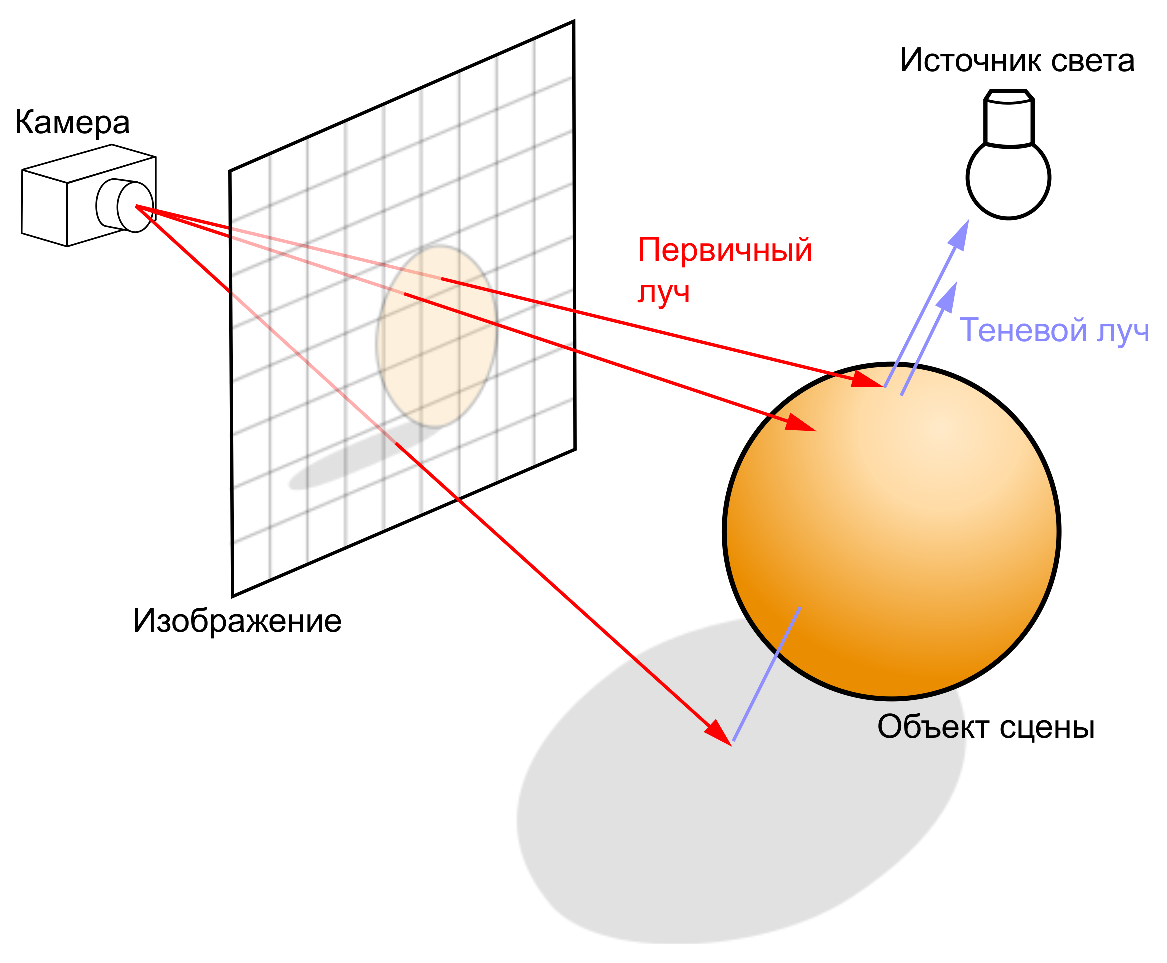
\includegraphics[width=\textwidth]{imgs/Ray_trace_diagram_rus.eps} 
\caption{Обратный метод трассировки лучей}\label{fig:alg_ray_tracing}
\end{figure}

Первый луч строится в направлении источника света. Если источников несколько, строится несколько таких лучей, по одному на каждый источник. Основное назначение этого луча – определить ориентацию точки (обращена ли точка к источнику), наличие объектов, закрывающих точку от источника света. Если точка обращена в противоположную сторону от источника света или закрыта другим непрозрачным объектом, освещенность от такого источника не рассчитывается, так как точка находится в тени. В случае затеняющего прозрачного объекта интенсивность освещения уменьшается в соответствии со степенью прозрачности. Если точка закрыта от освещения всеми источниками сцены, ей присваивается фоновый (\index{ambient}ambient) цвет. В противном случае точка освещена, интенсивность и цвет освещения рассчитываются при помощи локальной модели освещенности, как сумма освещенностей от всех источников, для которых эта точка не закрыта другими объектами. Этот тип луча получил название теневой луч (\index{ray!shadow}shadow ray или иногда его еще называют illumination ray\index{ray!illumination}). Если поверхность объекта не является отражающей и непрозрачна, теневой луч – единственный тип лучей который строится, траектория первичного луча обрывается (заканчивается), и дальнейшие расчеты не выполняются. Рассчитанный цвет присваивается тому пикселю видового окна, через который проходит соответствующий первичный луч.\par
   Второй луч строится, если поверхность объекта обладает отражающими свойствами, и называется луч отражения (\index{ray!reflection}reflection ray) или отраженный луч. Направление отраженного луча определяется по закону:
\begin{equation}
\vec{R} = \vec{I} - 2 \cdot \vec{N} (\vec{N} , \vec{I})
\label{eq_reflect}
\end{equation}
где $\vec{R}$ - отраженный луч, $\vec{I}$ - падающий первичный луч, $\vec{N}$ - нормаль к поверхности в точке соударения.
Для отраженного луча проверяется возможность пересечения с другими объектами сцены. Если пересечений нет, то интенсивность и цвет отраженного луча равна интенсивности и цвету фона. Если пересечение есть, то в новой точке снова строится три типа лучей – теневые, отражения и преломления.
Третий луч строится, если поверхность объекта прозрачна, и носит название преломленный луч (\index{ray!transparency}transparency ray). Направление для преломленного луча определяется следующим образом:
$$
 \vec{T} = \frac{n_1}{n_2} \cdot \vec{I} - \left[ \cos \alpha + \frac{n_1}{n_2} \cdot \left(\vec{N},\vec{I} \ \right) \right] \cdot \vec{N}
$$
$$
\cos \alpha = \sqrt{1 - \left( \frac{n_1}{n_2} \right) ^2 \cdot \left(1-\left(\vec{N},\vec{I}\ \right)^2\right)}
$$
где $\vec{T}$ - переломленный луч, $n_1$ - коэффициент рефракции для первой среды (в которой распространяется первичный луч), $n_2$ - коэффициент рефракции для второй среды прозрачного объекта.

Так же, как и в предыдущем случае, проверяется пересечение вновь построенного луча с объектами, и, если они есть, в новой точке строятся три луча.

Таким образом, для каждого первичного луча можно построить древовидную структуру. Если древовидная структура для данного луча построена, то расчет освещенности можно выполнить в следующем порядке. Для каждой ветви дерева спускаемся вдоль древовидной структуры к последнему пересечению вторичного луча и поверхности (будем дальше называть их узлами). Поскольку это последний узел в цепи, то  вкладов от преломлений и отражений нет, поэтому, освещенность узла вычисляется при помощи локальной модели освещения с учетом видимости источников света для данного узла. Затем, вычисленная освещенность передается вверх по ветви к следующему ближайшему узлу. Освещенность в этом узле будет вычисляться по формуле:

$$
 \vec{I}_{total} = \vec{I}_{local} + K_{reflection} \cdot \vec{I}_{reflection} + K_{refraction} \cdot \vec{I}_{refraction}
$$

где $\vec{I}_{total}$ - полная освещенность в точке, $\vec{I}_{local}$ - локальная освещенность в точке, вычисленная от источников освещения с помощью одной из локальной модели освещенности, $K_{reflection}$ - коэффициент, определяющий отражающие свойства поверхности, $\vec{I}_{reflection}$ - освещенность предыдущей точки, переданная вдоль ветки отражения, $K_{refraction}$ - коэффициент, определяющий преломляющие свойства поверхности $\vec{I}_{refraction}$ - освещенность предыдущей точки, переданная вдоль ветки преломления

Естественным завершением трассировки лучей является выход всех испущенных вторичных лучей за пределы видимой области и их рассеяние на чисто диффузных объектах. Результат вычислений будет наиболее точным. Но, если сцена достаточно сложна, такой расчет будет очень медленным, а в некоторых случаях и невозможным по причине ограниченности аппаратных ресурсов. Легко увидеть, что вклад освещенности от каждого нового вторичного луча очень быстро уменьшается по той простой причине, что коэффициенты свойств отражения и преломления материалов меньше единицы. Поэтому часто трассировку лучей прекращают, когда вклад от следующего узла ветви становится меньше заданной величины. Это также достаточно точный метод расчетов, который может быть использован для получения качественных результатов при определенных условиях. Наконец, для получения оценочного расчета можно оборвать трассировку лучей после выполнения заданного количества итераций, это самый быстрый и наименее точный расчет.

\subsubsection{Достоинства и недостатки}

Основные достоинства рекурсивного метода обратной трассировки лучей – расчет теней, многократных отражений и преломлений, значительно повысивших степень реалистичности получаемых изображений.

Основные недостатки:
\begin{itemize}
\item Отсутствие учета вторичного освещения от диффузно отраженного объектами света;
\item Низкая скорость и высокая вычислительная стоимость расчетов -- в классическом алгоритме трассировки лучей\index{трассировка лучей} необходимо проверять на пересечение каждый луч со всеми объектами сцены, в результате от 70 до 95 процентов всего времени расчетов тратится на вычисление пересечений;
\item Резкие границы цветовых переходов тени/подсветок/прозрачности;
\item Aliasing\index{aliasing} – <<зазубренность>>(ступенчатость) линий;
\item Дискретность определяющих цвет пиксела первичных лучей, т.е. одного первичного луча недостаточно для корректного определения цвета пиксела, формирующего изображение.
\end{itemize}

Однако от большинства недостатков можно избавится.

\subsection{Модели освещения}

В соответствии с принятым в компьютерной графике подходом, расчет освещенности распадается на две основные задачи. Первая -- определить способ расчета освещенности в произвольной точке трехмерного пространства, решается при помощи построения обобщенной математической модели освещения\index{модель!освещения} (illuminating model\index{model!illuminating!local}). Вторая задача -- применение illuminating model для компьютерных расчетов освещенности трехмерных объектов с конкретной геометрией и свойствами поверхности, решается при помощи так называемой модели затенения\index{модель!затенения} (shading model\index{model!shading}).

Моделей освещения к настоящему моменту разработано несколько. Самая первая и самая простая -- локальная модель освещения. Сама модель не рассматривает процессы светового взаимодействия объектов сцены между собой, а только расчет освещенности самих объектов. Вторая -- это глобальная модель освещенности\index{модель!глобальная} (global illuminations model\index{model!illuminating!global}), она рассматривает трехмерную сцену как единую систему и пытается описывать освещение с учетом взаимного влияния объектов. В рамках этой модели рассматриваются такие вопросы, как многократное отражение и преломление света, рассеянное освещение\index{рассеянное освещение} (radiosity\index{radiosity}), каустик\index{каустик}(caustic\index{caustic}) и фотонные карты\index{фотонные карты} (photon mapping\index{photon mapping}) и другие.

\subsubsection{Глобальные модели освещения}

Глобальное освещение\index{модель!глобальная} (global illumination model\index{model!illuminating!global}) -- это название ряда алгоритмов, используемых в 3D-графике, которые предназначены для добавления более реалистичного освещения в трёхмерные сцены. Такие алгоритмы учитывают не только свет, который поступает непосредственно от источника света, т.е. прямое освещение(model!illumination!direct), но и такие случаи, в которых лучи света от одного и того же источника, отражаются на других поверхностях сцены, т.е. непрямая освещенность(indirect illumination\index{model!illumination!indirect}).

Теоретически, отражение, преломление, тень — примеры глобального освещения, потому что, для их имитации необходимо учитывать влияние одного объекта на другие, в отличие от случая когда на объект падает прямой свет. На практике, только моделирование диффузного отражения или каустики называется глобальным освещением.

Изображения, полученные в результате применения алгоритмов глобального освещения часто кажутся более фотореалистичными, чем те, в процессе рендеринга которых, применялись алгоритмы только прямого освещения, но для просчета глобального освещения, требуется гораздо больше времени.

\subsubsection{Локальные модели освещения}

Существующие локальные модели освещения можно разделить на две категории. К первой категории относятся эмпирические модели. Они обычно эффективны в плане быстродействия и некоторые из них дают довольно реалистичную картинку. Они обычно не оперируют такими физическими величинами, как световая энергия, или световой поток. Однако эти модели находят довольно широкое применение в областях, где не требуется точная физическая информация об освещении (например, спецэффекты в фильмах, программы для художников и дизайнеров, для рекламных целей)

Ко второй категории относятся модели, базирующиеся на физических представлениях о теории света. Изображения, полученные с использованием этих моделей, очень хорошо соотносятся с экспериментальными данными. Поэтому, эти модели находят применение там, где важна точная имитация поведения света, например, при моделирование распространения света в помещение.

\subsubsection{Модель Фонга}

Модель Фонга -- это эмпирическая модель. В самом общем случае, в свете требований фотореалистичности, эта модель учитывает и неявное ambient-освещение. Ambient\index{ambient}-освещение, или его еще называют фоновым освещением (background), – это окружающее объект освещение от удаленных источников, чье положение и характеристики не известны. Необходимость учета ambient-освещения, пусть и очень грубо, обусловлена тем, что его вклад может быть достаточно велик – до 50\% от общей освещенности. В local illumination\index{model!illumination!local} считают, что фоновое освещение задает цвет (и его интенсивность) объекта в отсутствии явных источников света или в тени. Не несет никакой информации об объекте, кроме значения простого цвета, равномерно заливающего контур объекта.

Интенсивность такого освещения постоянна и равномерно распределена во всем пространстве, расчет его отражения поверхностью выполняется по формуле:

$$
 \vec{I}_{amb} = K_{a} \cdot \vec{I}_{a}
$$

где $\vec{I}_{amb}$  - интенсивность отраженного ambient освещения, $K_{a}$ - коэффициент, характеризующий отражающие свойства поверхности для  ambient-освещения, $\vec{I}_{a}$ - исходная интенсивность ambient-света, падающего на поверхность.

Часть света от прямых источников зеркально отражается поверхностью, а остальной свет диффузно рассеивается во всех направлениях. Кроме чисто зеркального отражения, которое имеют идеально отполированные поверхности, различают так называемое glossiness\index{glossiness} или распределенное зеркальное отражение – отражение в некотором створе углов, а не на один единственный угол. Такое рассеяние света обусловлено микрорельефом ("шероховатостью") поверхности, то есть поверхность реальных объектов не является идеально гладкой, а состоит из большого количества микровыступов и впадин, которые зеркально отражают падающий свет под разными углами. Результатом glossy-отражения является specular highlight\index{specular highlight} – яркий световой блик, имеющий размер в зависимости от степени шероховатости поверхности. 

Интенсивность рассеянного света зависит от угла падающего на поверхность света по закону Ламберта (Lambert)\index{закон Ламберта}:

$$
 \vec{I}_{diff} = K_{diff} \cdot \vec{I}_{d} \cdot \cos(\alpha)
$$
 
где $\vec{I}_{d}$ - интенсивность падающего на поверхность света, $K_{diff}$ - коэффициент, характеризующий рассеивающие свойства поверхности, $\cos(\alpha)$ - угол между направлением на источник света и нормалью поверхности

Другими словами, поверхность будет освещена больше, если свет падает на нее перпендикулярно ($\alpha = 0$), и меньше, если свет падает под любым другим углом, поскольку в этом случае увеличивается освещаемая площадь. Диффузно рассеянный свет является главным источником визуальной информации о геометрии трехмерных объектов.

Как было уже сказано ранее, свет отражается зеркально в некотором створе углов, и для большинства реальных материалов мы всегда видим зеркальную подсветку в форме светового пятна, а не в форме яркой точки. Поэтому, для расчета интенсивности зеркально отраженного света используется формула, предложенная Фонгом:

$$
 \vec{I}_{spec} = K_{spec} \cdot \vec{I}_{s} \cdot \cos^n(\beta)
$$

где $\vec{I}_{spec}$ - интенсивность зеркально отраженного света,  $\vec{I}_{s}$ - интенсивность источника света,  $\vec{K}_{s}$ - коэффициент, характеризующий свойства зеркального отражения поверхности
$\beta$ - угол между направлением идеального отражения и направлением на наблюдателя, степень $n$ определяет размер пятна светового блика, чем больше $n$, тем меньше световой блик, и тем ближе отражающие свойства поверхности к свойствам идеального зеркала.

Формула Фонга – пример компьютерной фикции, поскольку она не имеет физического смысла. Ее используют просто потому, что она дает хорошие практические результаты. 

Таким образом, локальная модель освещенности предполагает расчет отраженной фоновой освещенности, диффузного и зеркального отражения от прямых источников: 

$$
 \vec{I}_{local} =  K_{amb} \cdot \vec{I}_{amb} +  K_{diff} \cdot \vec{I}_{diff} \cdot \left( \vec{L},\vec{N} \right) + K_{spec} \cdot \vec{I}_{spec} \cdot \left( \vec{R},\vec{V} \right)^n
$$

\subsection{Модель камеры}

Для того что бы точно ориентировать камеру, необходимо указать следующие вектора:
\begin{itemize}
\item[$C_d$] - задает вектор направления, т.е. указывает, куда смотрит камера (в локальной модели координат)
\item[$C_p$] - задает точку в пространстве, определяющую положение камеры ( в общей модели координат)
\item[$C_u$] - задает вектор направления, указывая, где у камеры вверх (в локальной модели координат)
\item[$C_l$] - задает вектор направления, указывая, где у камеры лево (в локальной модели координат)
\end{itemize}

\subsubsection{Рассчет луча}

Для того, что бы построить исходящий луч, необходимо знать через какую точку $(x,y)$ видового окна пройдет луч.

\begin{figure}[H]
\centering
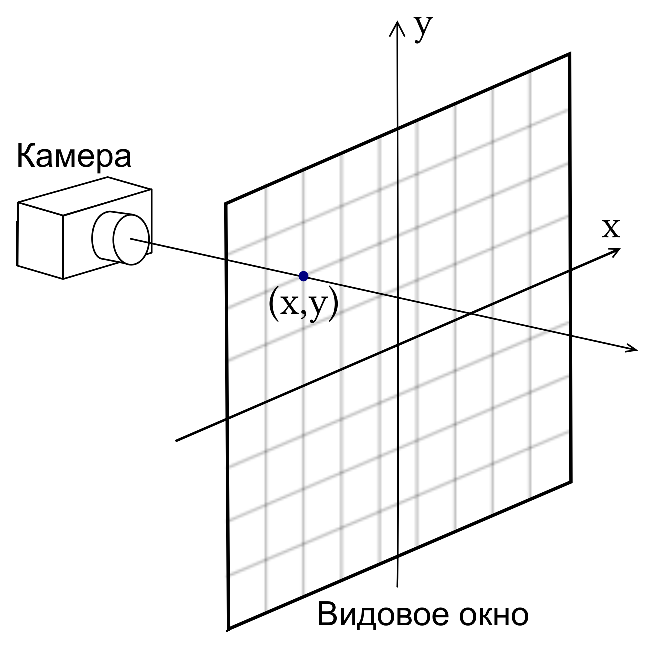
\includegraphics[scale=0.75]{imgs/camera.eps} 
\caption{Модель камеры}\label{fig:camera_model}
\end{figure}

Расчет луча осуществляется достаточно просто. Луч определяется 2 векторами: положением и направлением. Положение луча совпадает с положением камеры. А направление вычисляется слудующим образом.
Пусть необходимо рассчитать луч, для точки с координатами $(\hat x, \hat y) : 0 \le \hat x < width, 0 \le \hat y < height$
Для это преобразуем координаты $(\hat x, \hat y)$ в $(x, y) : -1 \le x \le 1, -1 \le y \le 1$:
\begin{equation*}
\begin{split}
x &= 2.0 \cdot (\hat x / width) - 1.0{}\\
y &= 1.0 - 2.0 \cdot (\hat y / height)
\end{split}
\end{equation*}
Учитывая соотношение сторон и угол раствора камеры:
\begin{equation*}
\begin{split}
aspect &= width / height \\
tan\_av &= \tg(angle\_of\_view \cdot rad\_to\_angle) \\
x &= x \cdot aspect \cdot tan\_av \\
y &= y \cdot tan\_av
\end{split}
\end{equation*}

Для получения направляющего вектора луча, осталось взять векторы камеры с соответствующими коэффициентами:
$$ 
dir = \normalize(C_d + C_l \cdot x + C_u \cdot y)
$$

\subsection{Антиалиасинг}

Как следует из приставки ''анти'', эта технология призвана бороться с алиасингом, т.е. со ''ступеньками''. Чтобы понять, что такое алиасинг\index{алиасенг}, необходимо понять самый общий принцип вывода изображения на экран монитора. Экран состоит из миллионов очень мелких квадратов (обычно, называемых точками или пикселями) - примерно как бумага в клетку, только гораздо мельче. Каждый квадрат (точка, пиксель, клетка) может быть закрашена только одним цветом.

\begin{figure}[H]
\centering

\includegraphics[scale=3]{imgs/aliasing.png} 
\caption{Пример шрифта без антиалиасинга}\label{fig:font_without_antialiasing}
\end{figure}

Обратите внимание, что рисунок, состоящий из таких больших точек, выглядит странно. Собственно, это и есть алиасинг - на краях букв видны ''ступеньки''. Самое очевидное решение проблемы - уменьшить точки. К сожалению, экран монитора имеет очень существенный недостаток: он не позволяет сделать точки настолько малыми, чтобы взгляд не мог их различить. 

\begin{figure}[H]
\centering

\includegraphics[scale=3]{imgs/antialiasing.png}
\caption{Пример шрифта с антиалиасингом}\label{fig:font_with_antialiasing}
\end{figure}

Однако, при помощи плавных переходов цветов на изображении, можно очень существенно сгладить ''ступеньки'', т.е. как бы компенсировать недостаток пространственного разрешения цветовым.

\begin{figure}[H]
\centering

\includegraphics[scale=1.0]{imgs/aliasing.png} 

\includegraphics[scale=1.0]{imgs/antialiasing.png}
\caption{Сравнение шрифта с алиасингом и антиалиасингом}\label{fig:compare_font}
\end{figure}

Сглаживание основывается на том, что каждый пиксель разбивается на несколько субпикселей. Цвет каждого пикселя определяется усреднением по какому-либо закону цветов всех субпикселей, которые находятся внутри пикселя. При этом, хотя физически разрешение остается прежним, эффективное разрешение значительно повышается. Именно на таком принципе борьбы с алиасингом основаны все современные методы анти-алиасинга, которые уже давно используются в игровых ускорителях.

Два наиболее часто применяемых подхода - это ''суперсэмплинг'' и ''мультисэмплинг''. Оба они основаны на том, что цвет каждого пикселя вычисляется путем смешивания цветов субпикселей (сэмплов). Но сэмплы в этих методах генерируются по-разному.

\textbf{Суперсэмплинг}(supersampling\index{supersampling}) - это самый простой и прямолинейный метод сглаживания. Он заключается в том, что изображение рассчитывается в виртуальном разрешении, в несколько раз превосходящем реальное экранное. После чего оно масштабируется и фильтруется до итогового разрешения. При этом цвет каждого пикселя реального разрешения вычисляется на основе нескольких субпикселей виртуального. Это позволяет значительно повысить качество изображения, но при этом нагрузка на ускоритель возрастает в несколько раз и скорость при этом, соответственно, падает. Вызвано это тем, что вместо одного цвета для пикселя, приходится рассчитывать в несколько раз больше.

\textbf{Мультисэмплинг} - гораздо более хитрый и интеллектуальный метод сглаживания. Правильнее это называть даже не метод, а скорее инструмент. Идея, по сути, очень проста: зачем просто так тупо вычислять N субпикселей для каждого пикселя? Ведь, уже рассчитанные субпиксели, во многих случаях, можно использовать несколько раз, для формирования не одного, а нескольких результирующих пикселей. С другой стороны, в некоторых участках изображения, сглаживание не требуется вовсе, так зачем рассчитывать их по нескольким субпикселям? Достаточно и одного. И, наоборот, в других участках нужно очень хорошее качество сглаживания и там можно рассчитать очень много субпикселей. Этот инструмент позволяет не только значительно сэкономить ресурсы ускорителя, но и получить лучшее качество сглаживания! Этот инструмент может использоваться как угодно и, качество сглаживания и скорость зависят от конкретной реализации, которую выбрал разработчик ускорителя или игры.

\subsubsection{Supersampling}
Несмотря на то, что мультисэмплинг является интеллектуальным методом сглаживанием, который позволяет съэкономить время вычисления, качество изображения может быть недостаточно хорошим. Если рассматиривать ''сглаживание'' только границ объектов,  то это позволяет повысить производительность, за счет того, что не происходит вичеслений вспомогательных субпикселей в случае, если это один объект. Но в в данном случае, могут иметь место отражения и тогда отражения будут выглядить ''ступеньками''. Поэтому был выбран алгоритм суперсэмплинг. 

В качестве паттерна для вычисления субпикселов была выбрана равномерная сетка, однако качество  получаемого изображения было не очень хорошим. Поэтому предложен новый паттерн, с помощью которого следует вычислять субпикселы - субпикселы выбирались по кругу внутри пиксела. 

\begin{figure}[H]
\centering
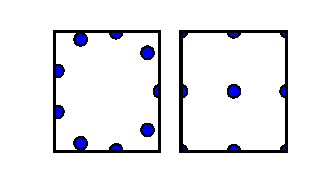
\includegraphics[scale=1]{imgs/aa_pattern.eps}
\caption{Паттерны расположения субпикселов}\label{fig:pattern_subpixel}
\end{figure}

Покажем почему данный шаблон лучше стандартного.

\begin{figure}[H]
\centering
{\hspace*{-2.35cm}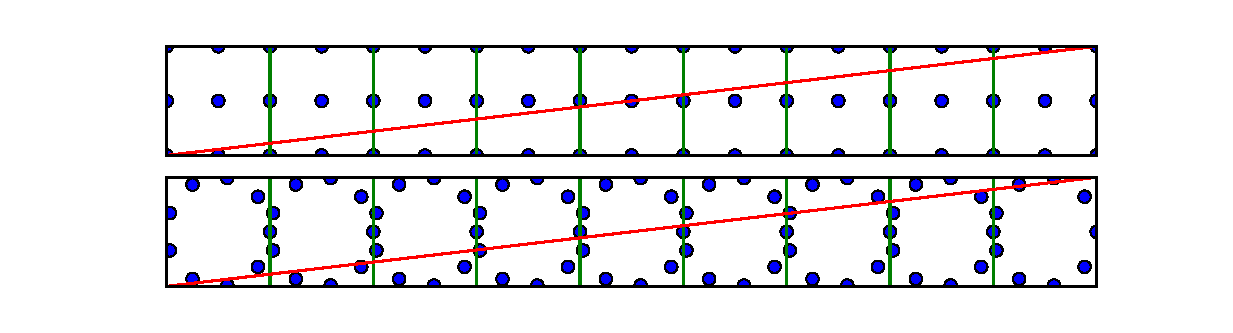
\includegraphics[scale=1]{imgs/aa_example.eps}}
\caption{Сравнение паттернов}\label{fig:compare_pattern_subpixel}
\end{figure}

Пусть необходимо отрендерить границу объекта, которая проходит ниже линии (см. рис. \ref{fig:compare_pattern_subpixel}). В случае со стандарным шаблоном, пикселы с 1 по 4 закрасятся одним цветом, т.к. в них одинаковое количество субпикселов. В новом паттерне заливка будет происходить более плавнее, при равном числе субпикселей.

\subsubsection{Результаты работы алгоритмов сглаживания}
Представлены результаты различных алгоритмов сглаживания.

\begin{figure}[H]
\centering

\includegraphics[scale=4]{imgs/aa_no.png}

\includegraphics[scale=4]{imgs/aa_std.png}

\includegraphics[scale=4]{imgs/aa_my.png}
\caption{Результаты сравнения паттернов}\label{fig:result_compare_pattern_subpixel}
Слева на право: без сглаживания; алгоритм с равномерной сеткой; алгоритм с точками по окружности
\end{figure}

\subsection{Примитивы}\index{примитив}
\subsubsection{Плоскость}\index{примитив!плоскость}
Для определения пресечения луча с плоскостью, необходимо найти точку в пространстве, которая будет удовлетворять двум уравнениям: уравнению луча и уравнению плоскости.
\par
Уравнение луча:
\begin{equation}
\left\{
\begin{array}{ccccc}
x & = & x_p & + & t \cdot x_d \\
y & = & y_p & + & t \cdot y_d \\
z & = & z_p & + & t \cdot z_d \\
\end{array}
\right.
\label{equation_ray}
\end{equation}
или
$$
\vec{R}(t) = \vec{P} + t \cdot \vec{D}
$$
где $\vec{P} = \VECXYZ{p} $ - начало луча, а $\vec{D} = \VECXYZ{d} $ - направление луча. 
\par
Уравнение плоскости задается следующим образом:
\begin{equation}
Ax + By + Cz + D = 0
\label{equation_plane}
\end{equation}
\par
Для того, что бы найти точку пересечения луча с плоскостью, необходимо подставить уравнение (\ref{equation_ray}) в (\ref{equation_plane}):
$$
A(x_p + t \cdot x_d) + B(y_p + t \cdot y_d) + C(z_p + t \cdot z_d) + D = 0
$$
Раскроем скобки и привидём подобные
$$
t(Ax_d + By_d + Cz_d ) + Ax_p + By_p + Cz_p + D = 0
$$
выразим неизвестную величину t:
$$
 t = - \frac{Ax_p + By_p + Cz_p + D}{Ax_d + By_d + Cz_d}
$$
из уравнения видно, что луч либо пересекает плоскость в какой то точке, либо нет. Это связано с тем, что если $Ax_d + By_d + Cz_d = 0$, то плоскость и луч параллельны друг другу. Т.к. $\vec{N} = \VEC{A}{B}{C} $ - это нормаль к поверхности, а из геометрии известно, что если $( \vec{D} , \vec{P} ) = 0$, то вектора параллельны.
\par
   Для того, что бы найти величину $t$, необходимо рассчитать всего несколько скалярных произведений:
$$
t = - \frac{(\vec{P}, \vec{N}) + D}{(\vec{D}, \vec{N})}
$$
при условии, что $(\vec{D}, \vec{N}) \neq 0$
\begin{codebox}
\Procname{ $\proc{Алгоритм нахождения точки пересечения луча и плоскости}$}
\li \If $(\vec{D}, \vec{N}) \neq 0$
\li \Then $ t = - \displaystyle\frac{(\vec{P}, \vec{N}) + D}{(\vec{D}, \vec{N})} $
\li $point = \vec{P} + t \cdot \vec{D}$
\end{codebox}

\subsubsection{Сфера}\index{примитив!сфера}
Для сферы необходимо проделать те же выкладки.
Уравнение сферы записывается следующем образом:
\begin{equation}
(x-x_c)^2 + (y-y_c)^2 + (z-z_c)^2 = r^2
\label{equation_sphere}
\end{equation}
где $\vec{C} = \VECXYZ{c}$ - центр сферы, а $r$ - радиус. Подставим уравнение (\ref{equation_ray}) в (\ref{equation_sphere}):
$$
\left( (x_0 + t \cdot x_d) - x_c \right)^2 + 
\left( (y_0 + t \cdot y_d) - y_c \right)^2 + 
\left( (z_0 + t \cdot z_d) - z_c \right)^2 = r^2
$$
раскроем скобки:
\begin{multline*}
(x_p + t \cdot x_d)^2 - 2(x_p + t \cdot x_d)\cdot x_c + x_c^2 + \\
 + (y_p + t \cdot y_d)^2 - 2(y_p + t \cdot y_d)\cdot y_c + y_c^2 + \\
 + (z_p + t \cdot z_d)^2 - 2(z_p + t \cdot z_d)\cdot z_c + z_c^2 = r^2
\end{multline*}
\begin{multline*}
x^2_p + 2x_px_d\cdot t + x_d^2 \cdot t^2 - 2 x_px_c - 2 x_dx_c \cdot t + x_c^2 + \\
 + y^2_p + 2y_py_d\cdot t + y_d^2 \cdot t^2 - 2 y_py_c - 2 y_dy_c \cdot t + y_c^2 + \\
 + z^2_p + 2z_pz_d\cdot t + z_d^2 \cdot t^2 - 2 z_pz_c - 2 z_dz_c \cdot t + z_c^2 = r^2
\end{multline*}

приведем уравнение в виду:
\begin{equation}
a \cdot t^2 + b \cdot t + c = 0
\label{equation_square}
\end{equation}
после раскрытия скобок и приведения подобных, получаем:
\begin{eqnarray*}
\begin{split}
a &= x^2_d + y^2_d + z^2_d \\
b &= 2x_px_d + 2 y_py_d + 2z_pz_d - 2x_dx_c - 2y_dy_c - 2z_dz_c \\
c &= x_p^2 + y_p^2 + z_p^2 - 2x_px_c - 2y_py_c - 2z_pz_c + x_c^2 + y_c^2 + z_c^2 - r^2 \end{split}
\end{eqnarray*}
упростим:
\begin{eqnarray*}
\begin{split}
a &= (\vec{D}, \vec{D}) \\
b &= 2x_d(x_0 - x_c) + 2y_d(y_0 - y_c) + 2z_d(z_0 - z_c) = 2 \cdot (\vec{D}, \vec{P}-\vec{C}) \\
c &= (x_0 - x_c)^2 + (y_0 - y_c)^2 + (z_0 - z_c)^2  - r^2 = 2 \cdot (\vec{P}-\vec{C},\vec{P}-\vec{C})
\end{split}
\end{eqnarray*}
перепишем в векторном виде
\begin{eqnarray*}
\begin{split}
a &= (\vec{D}, \vec{D}) \\
b &= 2 \cdot (\vec{D}, \vec{P}-\vec{C}) \\
c &= 2 \cdot (\vec{P}-\vec{C},\vec{P}-\vec{C}) - r^2
\end{split}
\end{eqnarray*}
Если уравнение (\ref{equation_square}) не имеет вещественных решений, то луч не пересекает сферу. Если имеется два решения, то наименьший положительный корень этого уравнения определит на луче ближайшую точку пересечения луча со сферой.
\par
Далее решаем обыкновенное квадратное уравнение, находим корни и получаем значение $t$,  при условие, что $a = (\vec{D},\vec{D}) \neq 0$
$$
t_{1,2} = \frac{-b \pm \sqrt{b^2 - 4 \cdot a \cdot c}}{2 \cdot a}
$$
\subsubsection{Треугольник}\index{примитив!треугольник}
Алгоритм пересечения луча и треугольника основан на барицентрических координатах.
\par
Барицентрические координаты\index{барицентрические координаты} -- координаты точки $n$-мерного аффинного пространства $A^n$, отнесенные к некоторой фиксированной системе из $(n + 1)$-ой точки $p_0, p_1, \dots, p_n$ , не лежащих в $(n -1)$-мерном подпространстве. Пусть $z$ есть произвольная точка в $A^n$. Каждая точка $x \in A^n$ может быть единственным образом представлена в виде суммы
$$
	x = z + \alpha_1 \cdot z\vec{p_1} + \alpha_2 \cdot z\vec{p_2} + \cdots + \alpha_n \cdot z\vec{p_n} 
$$
где $\alpha_1, \alpha_2, \dots,  \alpha_n $ вещественные числа, удовлетворяющие условию
$$
\alpha_1 + \alpha_2 + \cdots + \alpha_n  = 1
$$
Числа $\alpha_1, \alpha_2, \dots,  \alpha_n $ называются барицентрическими координатами точки $x$. Легко видеть, что барицентрические координаты не зависят от выбора $z$.
Точка $T(u,v)$, принадлежащая треугольнику, может быть записана в виде:
\begin{equation}
\label{triangle_bar}
T(u,v) = (1-u-v)V_0 + uV_1 + vV_2
\end{equation}
\noindent где $(u,v)$ -- это бариецентрические координаты такие, что $u \geq 0$, $v \geq 0$ и $u + v \leq 1$, а $V_0, V_1, V_2$ - это точки пространства, образующие треугольник.
Вычисление пересечения между лучем(\ref{equation_ray}) и треугольником(\ref{triangle_bar}), это решение следующего уравнения:
$$
\vec{P} + t\cdot \vec{D} = (1-u-v)\vec{V_0} + u\vec{V_1} + v\vec{V_2}
$$
после очевидных преобразований:
\begin{multline*}
\begin{split}
\vec{P} + t\cdot \vec{D} &= \vec{V_0} - u\vec{V_0} - v\vec{V_0} + u\vec{V_1} + v\vec{V_2} \\
\vec{P} - \vec{V_0} &= - t\vec{D} + u\vec{V_1} - u\vec{V_0} + v\vec{V_2} - v\vec{V_0} \\
- t\vec{D} &+ u(\vec{V_1} - \vec{V_0}) + v(\vec{V_2} - \vec{V_0}) = \vec{P} - \vec{V_0} \\
\end{split}
\end{multline*}
получаем:
\begin{equation}
\label{ray_cross_tr}
\left[ -\vec{D}, \vec{V_1} - \vec{V_0}, \vec{V_2} - \vec{V_0}\right] 
\left[  
\begin{array}{c} t \\ u \\ v \\ \end{array}
\right] = \vec{P} - \vec{V_0}
\end{equation}
Что бы решить задачу, необходимо найти вектор $\VEC{t}{u}{v}$. Обозначив $\vec{E_1} = \vec{V_1} - \vec{V_0}$, $\vec{E_2} = \vec{V_2} - \vec{V_0}$ и $\vec{T} = \vec{P} - \vec{V_0}$ решим уравнение (\ref{ray_cross_tr}), используя метод Крамера:
\begin{equation}
\label{ray_cross_tr_solv}
\left[  
\begin{array}{c} t \\ u \\ v \\ \end{array}
\right] = 
\frac{1}{| -\vec{D}, \vec{E_1}, \vec{E_2}|} 
\left[  
	\begin{array}{lcccl}
	|& \vec{T} , & \vec{E_1}, &\vec{E_2} & | \\
	|&-\vec{D} , & \vec{T}  , &\vec{E_2} & | \\
	|&-\vec{D} , & \vec{E_1}, &\vec{T}   & | \\
	\end{array}
\right] 
\end{equation}
Из курса линейной алгебры известно, что: $|A, B, C| = - (A \times C) \cdot B = - (C \times B) \cdot A$. Принимая во внимания этот факт, перепишем уравнение (\ref{ray_cross_tr_solv}).
\begin{equation}
\label{ray_cross_tr_solv2}
\left[  
\begin{array}{c} t \\ u \\ v \\ \end{array}
\right] = 
\frac{1}{(\vec{D} \times \vec{E_2})\cdot \vec{E_1}} 
\left[  
	\begin{array}{c}
	(\vec{T} \times \vec{E_1}) \cdot \vec{E_2} \\
	(\vec{D} \times \vec{E_2}) \cdot \vec{T} \\
	(\vec{T} \times \vec{E_1}) \cdot \vec{D} \\
	\end{array}
\right] = 
\frac{1}{(\vec{S}, \vec{E_1})} 
\left[  
	\begin{array}{c}
	(\vec{Q}, \vec{E_2}) \\
	(\vec{S}, \vec{T}) \\	
	(\vec{Q}, \vec{D}) \\	
	\end{array}
\right]
\end{equation}
где $\vec{S} = (\vec{D} \times \vec{E_2})$ и $\vec{Q} = (\vec{T} \times \vec{E_1})$

На этом можно остановится, однако можно заметить, что $ (E_1 \times E_2) $ это нормаль к треугольнику, которую можно заранее предвычислить. 
Запишем решение по другому:
\begin{eqnarray*}
\begin{split}
| -\vec{D}, \vec{E_1}, \vec{E_2} | & = -\vec{D} \cdot (\vec{E_1} \times \vec{E_2}) = -\vec{D} \cdot \vec{N}\\
| \vec{T}, \vec{E_1}, \vec{E_2} | & = \vec{T} \cdot (\vec{E_1} \times \vec{E_2}) = \vec{T} \cdot \vec{N}\\
| -\vec{D}, \vec{T}, \vec{E_2} | & = (\vec{T} \times -\vec{D}) \cdot \vec{E_2} = \vec{\hat{Q}} \cdot \vec{E_2}\\
| -\vec{D}, \vec{E_1}, \vec{T} | & = - | - \vec{D}, \vec{T}, \vec{E_1} | = -(-\vec{D} \times \vec{T} ) \cdot \vec{E_1} = - \vec{\hat{Q}} \cdot \vec{E_1}\\
\end{split}
\end{eqnarray*}
где 
$\vec{\hat{Q}} = -\vec{D} \times \vec{T}$.

Тогда вычисление по формуле (\ref{ray_cross_tr_solv2}) можно переписать так:
\begin{equation*}
\left[  
\begin{array}{c} t \\ u \\ v \\ \end{array}
\right] = 
\frac{1}{(-\vec{D} \cdot \vec{N})} 
\left[  
	\begin{array}{c}
	(\vec{T}, \vec{N}) \\
	(\vec{\hat{Q}}, \vec{E_2}) \\	
	(-\vec{\hat{Q}}, \vec{E_1}) \\	
	\end{array}
\right]
\end{equation*}
где 
$\vec{E_1} = \vec{V_1} - \vec{V_0}$,
$\vec{E_2} = \vec{V_2} - \vec{V_0}$,
$\vec{T}   = \vec{P} - \vec{P}$,
$\vec{N} = (\vec{E_1} \times \vec{E_2})$,
$\vec{\hat{Q}} = (-\vec{D} \times \vec{T})$.


Таким образом мы избавились от одной операции векторного умножения (фактически она осталась, но мы можем ее подсчитать заранее). 
Для того, что бы еще улучшить данный алгоритм и избавится от знака минус, произведем несколько замен:
\begin{eqnarray*}
\begin{split}
\vec{\tilde {E_1}} &= -\vec{E_1} = \vec{V_0} - \vec{V_1}\\
\vec{\tilde {E_2}} &= \vec{E_2} = \vec{V_2} - \vec{V_0}\\
\vec{\tilde {T}} &= -\vec{T} = \vec{V_0} - \vec{P}\\
\vec{\tilde {N}} &= -\vec{N} = - (\vec{E_2} \times \vec{E_1}) = (\vec{E_2} \times -\vec{E_1}) = (\vec{\tilde {E_2}} \times \vec{\tilde{E_1}}) \\
\vec{ \tilde{ Q } } &= - \vec{D} \times \vec{T} = - ( \vec{D} \times \vec{T}) = - ( \vec{D} \times ( - \vec{\tilde{T}})) = ( \vec{D} \times \vec{\tilde{T}} ) \\
-\vec{D} \cdot \vec{N} &= (-\vec{D} \cdot (-\vec{\tilde{N}})) = (\vec{D} \cdot \vec{\tilde{N}}) \\
\vec{T} \cdot \vec{N} &= (-\vec{\tilde{T}}) \cdot (-\vec{\tilde{N}}) = (\vec{\tilde{T}} \cdot \vec{\tilde{N}}) \\
\vec{\hat{Q}} \cdot \vec{E_2} &= (-\vec{D} \times \vec{T}) \cdot \vec{E_2} = (\vec{\tilde{T}} \times \vec{D}) \cdot \vec{\tilde{E_2}} \\
-\vec{\hat{Q}} \cdot \vec{E_1} &= (\vec{\tilde{T}} \times \vec{D}) \cdot \vec{\tilde{E_1}}
\end{split}
\end{eqnarray*}

В результате получаем следующие решение:

\begin{equation}
\label{ray_cross_tr_solv_fin}
\left[  
\begin{array}{c} t \\ u \\ v \\ \end{array}
\right] = 
\frac{1}{(\vec{D} \cdot \vec{\tilde{N}})} 
\left[  
	\begin{array}{c}
	(\vec{\tilde{T}} \cdot \vec{\tilde{N}}) \\
	(\vec{\tilde{S}} \cdot \vec{\tilde{E_2}}) \\	
	(\vec{\tilde{S}} \cdot \vec{\tilde{E_1}}) \\	
	\end{array}
\right]
\end{equation}
где 
$\vec{\tilde {E_1}} = \vec{V_0} - \vec{V_1}$,
$\vec{\tilde {E_2}} = \vec{V_2} - \vec{V_0}$,
$\vec{\tilde {T}}  = \vec{V_0} - \vec{P}$,
$\vec{\tilde{S}} = \vec{\tilde{T}} \times \vec{D}$,
$\vec{\tilde {N}} = (\vec{\tilde {E_2}} \times \vec{\tilde{E_1}})$.

\begin{codebox}
\Procname{ \proc{Алгоритм нахождения точки пересечения луча и треугольника}}
\li Вычисляем по формуле (\ref{ray_cross_tr_solv_fin}) вектор $\left[ \begin{array}{c} t \\ u \\ v \\ \end{array} \right]$
\li \If $(u \geq 0) \ \&\& \ (v \geq 0) \ \&\& \ (u + v \leq 1)$
\li \Then $point = \vec{P} + t \cdot \vec{D}$
\end{codebox}

\cppsource{src/triangle.tex}{Реализация алгоритма пересечения луча и треугольника}

%%%%%%%%%%%%%%%%%%%%%%%%%%%%%%%%%%%%%%%%%%%%%%%%%%%%%%%%%%%%%%%%%%%%%%%%%%%%%%%%%%%%%%%%%%%

\newpage
\section{Оптимизация}
Оптимизация -- как способ программирования по уровням архитектуры сверху вниз.

\subsection{Шаблоны C++}

\subsubsection{Понятие шаблона}

Шаблоны(Templates\index{templates}) были введены в язык C++ как средство, позволяющие параметризовать типы данных. Это связано с тем, что для классов или функций приходилось реализовывать одни и те же алгоритмы, но для разных типов данных. Получали дублирование кода, и тем самым росло число ошибок. 
Пример. Реализовать функцию, которая возвращает максимальное значение из 2 чисел.

\cppsource{src/deftemplate.tex}{Несколько реализация функции {\bf max}}

\noindent
и так далее. Приходится писать один и тот же код несколько раз. Во второй функции можно было допустить ошибку (например указать неправильный знак сравнения), которую потом очень трудно найти. Или наоборот, после обнаружения ошибки, придется править код во всех реализациях функции max (возможна ситуация, когда в нескольких местах ошибка была исправлена, а в остальных пропущена или забыта). С этими проблемами помогли справится шаблоны, которые параметризовали типы данных следующим образом:

\cppsource{src/definetemplate.tex}{Шаблонное определение функции {\bf max}}

%\noindent
Таким образом работу, которую выполнял программист теперь выполняет компилятор. При вызове функции, в качестве параметров которых нужно сравнить два int, компилятор сам из шаблона выведет функцию max(int,int).
\subsubsection{Вычисление на шаблонах. Факториал}
Сегодня шаблоны используют различным образом, не так как ожидали изобретатели
шаблонов С++. Сегодня программирование на шаблонах включают различные техники, такие как: обобщенное программирование, вычисление во время компиляции, шаблонные выражения(expression templates), мета-программирование, и др.

\noindent Рассмотрим пример вычисления факториала. \\
\noindent Факториал числа N это: $N! = N \cdot (N-1) \cdot \dots \cdot 1$

Рекурсивная реализация факториала, без использование шаблонов, приведена в следующем листинге:

\cppsource{src/rekfactorial.tex}{Рекурсивная реализация факториала}

Эту функцию следует использовать следующим образом:
\begin{verbatim}
cout << factorial(7) << endl;
\end{verbatim}
Вызывать рекурсивно функцию - это очень большие накладные расходы. Несмотря на то, что мы указало компилятору встроить функцию (inline), компилятор проигнорирует это, так как он не может сделать постановку в рекурсию. Можно добиться большего успеха, если реализовывать это, как класс с шаблоном.

\cppsource{src/templatefactorial.tex}{Реализация факториала на шаблонах}

Можно заметить, что у данного шаблона нет ни данных, ни функциональных участков, это только определение перечислимого типа. Для того чтобы можно было определить шаблон для n, нужно для начала определить шаблон для n-1, т. е. для n-2, n-3 и т. д. В итоге получаем рекурсию. Следует заметить, что в качестве параметра шаблона используется обычный тип int. По стандарту, в качестве параметров шаблона могут быть использованы только перечислимые типы. В нашем случае есть параметр шаблона типа int, это означает, что в этот шаблон будет подставлено постоянное число типа int. Что бы воспользоваться данным классом необходимо написать следующие:
\begin{verbatim}
cout << factorial<7>::ret << endl;
\end{verbatim}
Компилятор рекурсивно определяет значение факториала<7>, затем <6> и так далее. Так как это рекурсия, то что бы не зациклится необходимо вовремя остановится. Любая рекурсия нуждается в остановки, и это не исключение. Это можно сделать с помощью специализации шаблона(т.е. определение для частного случая).

\cppsource{src/specfactorial.tex}{Специализация шаблона вычисления факториала}

Когда компилятор начнет определять специализацию для <0>, то он подставит имеено эту реализацию и рекурсия завершится. В результате, получится следующая структура:

\cppsource{src/finfactorial.tex}{Развернутая структура вычисления факториала}

Как видно из примера, от структуры уже ничего ни осталось и при уровне оптимизации начиная с O1, компилятор подсчитает выражение и вместо:
\begin{verbatim}
cout << factorial<7>::ret << endl;
\end{verbatim}
Подставит, подсчитанное выражение:
\begin{verbatim}
cout << 5040 << endl;
\end{verbatim}

Разумеется, если мы используем шаблоны подобным образом, то это замедляет процесс сборки приложения, но ускоряет работу программы. Проверить результат  это можно дизассемблировав данный пример и увидеть в коде число 5040.

\subsubsection{Вычисление на шаблонах. Квадратный корень}
Например: $\sqrt{10} \approx 3.1622776601 $. Округлим в большую сторону и получим 4.
Воспользуемся общей формулой для вычисления корня степени~$n$:
$$
x_{k+1} = \frac{1}{n}\left[ (n-1)x_k + \frac{A}{x_k^{n-1}} \right]
$$

Если $k=\infty$, то $x_k = \sqrt[n]{A}$, тогда для $n=2$:
$$
x_{k+1} = \frac{1}{2}\left[ x_k + \frac{A}{x_k} \right]
$$

\noindent 
Воспользуемся данной формулой и напишем следующую шаблонную структуру:
\cppsource{src/defroot.tex}{Шаблонное определение структуры root}

Рассмотрим подробнее, как это работает. Значение $ret$ возвращает очередное приближение значения корня. Для начала необходимо вычислить очередное приближение. Запишем его в переменную $calc$, вычисленную как очередной шаг. Далее необходимо провести тест и понять, данное число в квадрате получилось больше $N$ или меньше. Если полученное число больше $N$, то следующие приближение нужно искать на отрезке от $Low$ до $calc$, иначе на отрезке от $calc+1$ до $Upp$. Каждую итерацию отбрасываем часть отрезка, тем самым приближаясь к ответу. Т. к. значения $Low$ и $Upp$ это целый тип данных, то состояний конечное число, и из этого следует, что процесс остановится когда $Low$ и $Upp$ будут равны. Поэтому, для остановки, запишем следующую специализацию шаблона: 

\cppsource{src/defrootsp.tex}{Специализация структуры root}

Теперь этот шаблон можно использовать следующим образом:
\begin{verbatim}
cout << Root<10>::ret << endl;
\end{verbatim}
Из примеров видно, что очень часто вычисление во время компиляции это рекурсивные задачи.

\subsubsection{Шаблонные выражения(expression templates)}
Expression templates или шаблоны выражений -- это специальная техника в программировании на языке C++, которая использует шаблоны для разбора выражений во время компиляции.

\cppsource{src/defvector.tex}{Определение структуры vector}

\noindent 
Тогда сумму 3-х веторов можно записать так:
\begin{verbatim}
static const int db[8] = {1, 1, 1, 1, 1, 1, 1, 1};
vector<int> a(8,db), b(8,db), c(8,db);
static vec d(8);
d = a + b + c;
\end{verbatim}

Недостатки данного подхода заключаются в том, что необходимо дополнительная память в виде 2-х векторов для вычисления этого выражения, т. е. Это выражение будет вычислено следующим образом: 

\begin{verbatim}
vector<int> t1(8), t2(8);
t1 = a + b;
t2 = t1 + c;
\end{verbatim}

Так же будут сделаны вызовы функций: (operator+) 2 раза и 4 раза будут вызваны операторы (new/delete), итого 6 вызовов функций, плюс 1 функция копирования из вектора t2 в вектор d, при это будут сделаны 3+3+1=7 проходов по памяти. При больших векторах это может сильно повлиять на производительность.

	Что же предлагает нам Expression Templates(ET)? А именно всего 4 прохода по памяти (т. к. 4 вектора), вызов одной функции и никаких временных объектов и операций копирования. Как же это возможно? Expression templates или шаблоны выражений – это специальная техника в программировании на языке C++, которая использует шаблоны для разбора выражений во время компиляции. Т.о. сумма 3-х векторов:
\begin{verbatim}
d = a + b + c;	
\end{verbatim}
переходит в следующий код:
\begin{verbatim}
for(std::size_t i = 0; i < size; ++i)
    d[i] = a[i] + b[i] + c[i];
\end{verbatim}

Данную технику можно реализовать следующим образом. Для начало опишем новый класс векторов:

\cppsource{src/defvectoret.tex}{Определение структуры vector с ET}

Данный класс очень похож на класс, который был продемонстрирован выше, но все же с отличием. Перегружен специальным образом оператор присваивания. Это сделано для того, что бы каждому элементу $data[i]$ вычислить выражение стоящие в правой части выражения. Подробнее рассмотрим, что же это за выражение и каким образом к нему применимы операции ($expr[i]$).

\cppsource{src/defx.tex}{Определение структуры X}

В данном случае структура X может быть рассмотрена как арифметическое выражение записанное в виде дерева(листья - числа, узлы — арифметические операции). Самый первый шаблон определяет, что новое дерево(выражение), это выражение, которое равно левое подвыражение, далее операция и правое подвыражение. Для операции так же необходимо описать свой класс следующим образом:

\cppsource{src/defplus.tex}{Определение структуры plus}

Используя данные структуры, компилятор самостоятельно разберет выражение в качестве дерева и с оптимизирует полученное выражение. Таким образом мы значительно выигрываем по скорости работы, но трудность разработки таких классов достаточна велика. Остальные шаблоны описывают различные комбинации левых и правых частей в выражении. Использование таких шаблонов ничем не отличается от обычных классов векторов. 

\subsection{SIMD инструкции}

Применение SIMD инструкций в классе vec4.
\subsubsection{Базовые операции в классе vec4}

\subsubsection{Скалярное произведение векторов}

\subsection{Ускоряющие структуры}

При работе с большими сценами часто возникает необходимость в различных запросах, связанных с пространственным расположением объектов сцены. 

\noindent 
Типичными примерами подобных запросов являются : 
\begin{itemize}
\item определение объектов, пересекаемых заданным лучом
\item определение ближайшего объекта, пересекаемого заданным лучом
\item определение столкновения объектов между собой
\end{itemize}

Подобные запросы обычно имеют сложность $O(n)$, где $n$ - общее количество объектов в сцене. Из этого видно, что для больших сцен метод ''грубой силы''  (т.е. прямого перебора) просто неприемлем из-за своих больших затрат. Таким образом, возникает необходимость в методах с сублинейной сложностью (от общего количества объектов), а в идеале - когда сложность метода прямо пропорциональна количеству объектов, найденных данным запросом. Стандартным приемом, позволяющим заметно снизить сложность запросов о взаимном расположении объектов в пространстве, являются различные типы так называемых пространственных индексов. 
	Пространственный индекс - это некоторая структура данных (чаще всего иерархическая), строящаяся обычно на этапе подготовки сцены.

В качестве ускоряющей структуры было выбрано дерево BVH

\subsubsection{Алгоритм построения BVH}

\subsubsection{Алгоритм траверса луча через BVH}

%%%%%%%%%%%%%%%%%%%%%%%%%%%%%%%%%%%%%%%%%%%%%%%%%%%%%%%%%%%%%%%%%%%%%%%%%%%%%%%%%%%%%%%%%%%

\newpage
\section{Постановка и результаты экспериментов}

Эксперименты проводились на 6 ядерном компьютере с процессором Intel Core i7 980x с частотой 3.33GHz, оперативной памятью 12 Гб, ОС - Calculate Linux 11.3 x64. 

Intel Core i7 980X -- это процессор семейства Gulftown вышедшего в 2010 году. Основные характеристики представлены с помощью программы CPU-Z\footnote{CPU-Z -- это бесплатное программное обеспечение, которое показывает информацию об основных устройствах в системе (\href{http://www.cpuid.com/softwares/cpu-z.html}{http://www.cpuid.com/softwares/cpu-z.html})} на рис.~\ref{fig:cpuz}.

\begin{figure}[h]
\centering
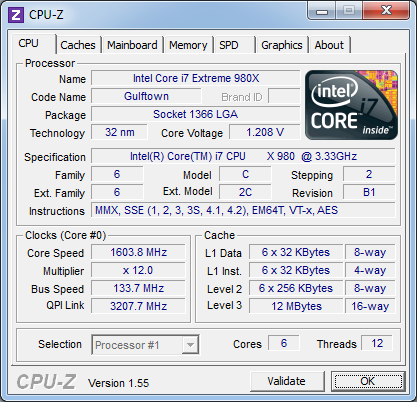
\includegraphics[scale=1]{imgs/cpu-z.png}
\caption{Основные характеристики процессора}\label{fig:cpuz}
\end{figure}

Для сборки приложения с библиотекой tbb, необходимо, что бы компилятор поддерживал лямбда выражения из нового стандарта c++0x. На данный момент, этот стандарт поддерживает компилятор GCC 4.5.2

\subsection{Timer}
Для того, чтобы точно оценивать время работы каждого из алгоритмов, очень важно иметь высокоточный таймер. Проблема в том, что стандартные методы операционных систем не работают с нужной точностью. Когда идет речь о том, чтобы оценить время, алгоритма который должен исполнятся очень много миллионов раз в секунду, важен каждый такт процессора и точность в секундах просто неприемлема.

Для очень точной оценки времени работы алгоритмов, был специально написан высокоточный таймер на языке c++, с использованием вставок на AT\&T ассемблере.
Таймер выдает время в тактах процессора и включает в себя разные режимы подсчета времени.

%{\hspace*{-2.25cm}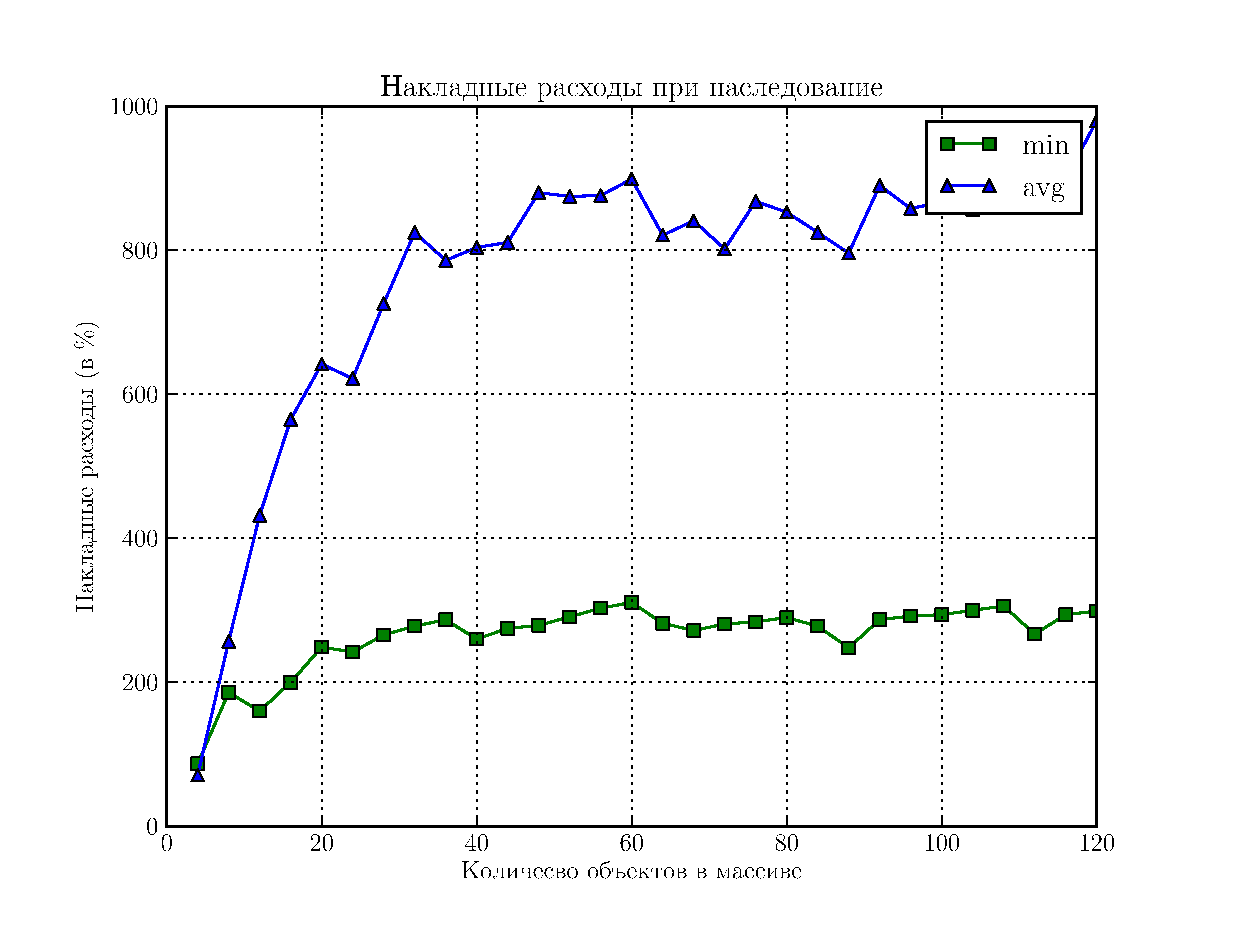
\includegraphics[scale=1]{apps/compare_virtual_methods_l.eps} }

\subsubsection{Алгоритм работы высокоточного таймера}
Основной код, выполняющий замеры времения приведен ниже.
\cppsource{src/timer.tex}{Метод Start() и Stop() класса Timer}

Рассмотрим его по порядку. Для того что бы начать отсчет времени, необходимо вызвать метод Start(). 
Вначале необходимо вызвать инструкцию cpuid, для того что бы процессор не менял порядок исполнения инструкций. Затем, вызывая инструкцию rdtsc, происходит запись количества тактов процессора в регистры edx и eax, которые и сохраняются в классе.
При вызове метода Stop(), 
Иснтрукция rdtscp читает значение значение количества тактов процессора и сохраняет их в регистры edx и eax, гарантируя при этом, что весь код, который находится о этой инструкции будет выполнен. После данной инструкции, так же стоит вызвать инструкцию cpuid, что бы предотвратить внеочередное исполнение инструкций.
Следует заметить, что на "замеряемое"\ время это ни как не повлияет, т.к. инструкция cpuid следует за инструкцией rdtscp\footnote{rdtscp - инструкция появилась лишь в процессорах Intel Core i7}. Далее просиходит вычисление разности времения в тактах между вызовом Start() и Stop(), и вызывается функция CalcSec() для вычисления времени в разных режимах отсчета времени.

Причины использования инструкции rdtscp состоит в том, что при использование rdtsc сама инструкция могла выполнится позже, чем ожидалось, что вносила ошибку в вычисления времени.

Функции Start() и Stop() объявлены как inline и по размеру представляют собой всего несколько ассемблерных инструкций, то код будет заинлайнен и вызовов функций происходить не будет, что положительно скажется на качестве таймера - нет накладных расходов. Убедится в этом можно дезассемблировать код с применением класса таймер.

\subsubsection{Эксперименты с высокоточным таймером}

\subsection{Вектора и Expression Templates}

\subsubsection{Оптимизация метода reflect}

Посмотрим на результаты применения техники Expression Templates. По формуле~(\ref{eq_reflect}) на стр.~\pageref{eq_reflect} запрограммируем метод reflect.

\cppsource{src/cpp_reflect.tex}{Исходный код метода reflect}

После компиляции с ключами оптимизации, было невозможно найти ассемблерный код соответствующей исходному, т.к. от получился встраиваемый(inline). Пришлось пойти на хитрость и вызвать данную функцию между двумя функциями, которые не могут быть встроены.
Поэтому, получаемый ассемблерный код берем между двумя вызовами метода (callq
407000 <\_ZN3rt25Scene10get\_lightsEv>)

Посмотрим на ассемблерный код.

\cppsource{src/asm_reflect.tex}{Метод reflect}

Как можно видеть, команды, которые вычисляют непосредственно выражение это строки [07-11] включительно. 
Если был бы использован класс std::valarray, то нам потребовалось бы 16 операций = 9 умножений + 3 сложения + 4 вычитания. А в оптимизированном случае получили всего 5 инструкций.

\subsubsection{Результаты вычисления арифметических выражений}

\begin{equation}
\vec{R} = \left(b - \frac{3}{4} \cdot a, b \cdot \left(a, b - a\right)\right) \cdot b + \frac{1}{400} \cdot a \cdot b \cdot \left(a, b\right)
\label{test_equation}
\end{equation}

{\small \begin{center}
\begin{longtable}{|c|c|c|c|c|}
\hline & \multicolumn{4}{c|}{Режим подсчета} \\ 
\hline \vbox{\hbox{\strut Кол-во}\hbox{итераций}} & min & avg & max & sum\\ 
\hline $10^1$ & $\cfrac{\strut 97}{\strut 2815} = 29.02 $ & $\cfrac{\strut 180}{\strut 3196} = 17.76 $ & $\cfrac{\strut 691}{\strut 6355} = 9.20 $ & $\cfrac{\strut 1813}{\strut 33412} = 18.43 $\\ 
\hline $10^2$ & $\cfrac{\strut 97}{\strut 2818} = 29.05 $ & $\cfrac{\strut 107}{\strut 4080} = 38.13 $ & $\cfrac{\strut 688}{\strut 11124} = 16.17 $ & $\cfrac{\strut 10593}{\strut 314672} = 29.71 $\\ 
\hline $10^3$ & $\cfrac{\strut 78}{\strut 2815} = 36.09 $ & $\cfrac{\strut 98}{\strut 2841} = 28.99 $ & $\cfrac{\strut 691}{\strut 6370} = 9.22 $ & $\cfrac{\strut 98761}{\strut 2837949} = 28.74 $\\ 
\hline $10^4$ & $\cfrac{\strut 78}{\strut 2815} = 36.09 $ & $\cfrac{\strut 97}{\strut 2835} = 29.23 $ & $\cfrac{\strut 8200}{\strut 15397} = 1.88 $ & $\cfrac{\strut 978827}{\strut 27306012} = 27.90 $\\ 
\hline $10^5$ & $\cfrac{\strut 72}{\strut 2845} = 39.51 $ & $\cfrac{\strut 98}{\strut 2766} = 28.22 $ & $\cfrac{\strut 7245}{\strut 35664} = 4.92 $ & $\cfrac{\strut 9897131}{\strut 282987948} = 28.59 $\\ 
\hline $10^6$ & $\cfrac{\strut 75}{\strut 2848} = 37.97 $ & $\cfrac{\strut 97}{\strut 2889} = 29.78 $ & $\cfrac{\strut 11018}{\strut 57837} = 5.25 $ & $\cfrac{\strut 98043177}{\strut 2828956136} = 28.85 $\\ 
\hline \caption{Времени выполнения арифметических выражений}\label{tab:cmp_et}\end{longtable}
\end{center}

 }

\subsection{Тестовая сцена}
\begin{figure}[H]
\centering
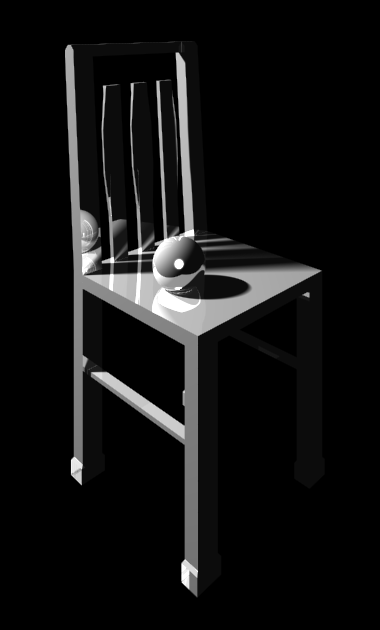
\includegraphics[scale=0.5]{imgs/stul.png}
\caption{Тестовая сцена}\label{fig:test_scene}
\end{figure}

\subsection{Эффективность расспаралеливания}

\begin{center}
\begin{longtable}{|c|p{2cm}|p{2cm}|p{2cm}|p{2cm}|}
\hline & \multicolumn{4}{c|}{Сложность сцены (fps)} \\ 
\hline Кол-во потоков & low & middle & hard &  very hard\\ 
\hline 1 &  8.179 & 2.49 & 0.473 & 0.304 \\ 
\hline 2 &  16.338 & 5.053 & 0.974 & 0.6 \\ 
\hline 3 &  23.996 & 7.468 & 1.478 & 0.906 \\ 
\hline 4 &  32.46 & 10.108 & 1.975 & 1.207 \\ 
\hline 5 &  40.288 & 12.384 & 2.473 & 1.508 \\ 
\hline 6 &  48.267 & 14.801 & 2.913 & 1.783 \\ 
\hline 7 &  36.397 & 11.222 & 2.361 & 1.496 \\ 
\hline 8 &  41.053 & 12.802 & 2.676 & 1.659 \\ 
\hline 9 &  46.097 & 14.306 & 2.872 & 1.849 \\ 
\hline 10 &  50.566 & 15.969 & 3.143 & 1.938 \\ 
\hline 11 &  55.624 & 17.239 & 3.412 & 2.12 \\ 
\hline 12 &  59.927 & 18.441 & 3.572 & 2.161 \\ 
\hline 13 &  50.836 & 15.828 & 3.372 & 1.929 \\ 
\hline 14 &  51.794 & 16.884 & 3.27 & 2.002 \\ 
\hline 15 &  52.457 & 17.318 & 3.397 & 2.089 \\ 
\hline 16 &  54.396 & 17.263 & 3.396 & 2.073 \\ 
\hline 17 &  55.403 & 16.927 & 3.469 & 2.134 \\ 
\hline 18 &  57.493 & 18.049 & 3.523 & 2.144 \\ 
\hline 19 &  55.728 & 17.488 & 3.474 & 2.18 \\ 
\hline 20 &  55.969 & 17.536 & 3.527 & 2.188 \\ 
\hline 21 &  55.327 & 17.418 & 3.577 & 2.187 \\ 
\hline 22 &  57.465 & 17.935 & 3.547 & 2.194 \\ 
\hline 23 &  57.521 & 18.043 & 3.6 & 2.233 \\ 
\hline 24 &  57.895 & 17.747 & 3.537 & 2.167 \\ 
\hline
\caption{Производительность реализации параллельного алгоритма}\label{tab:perf_parallel_alg}\end{longtable}
\end{center}



\begin{figure}[H]
\centering
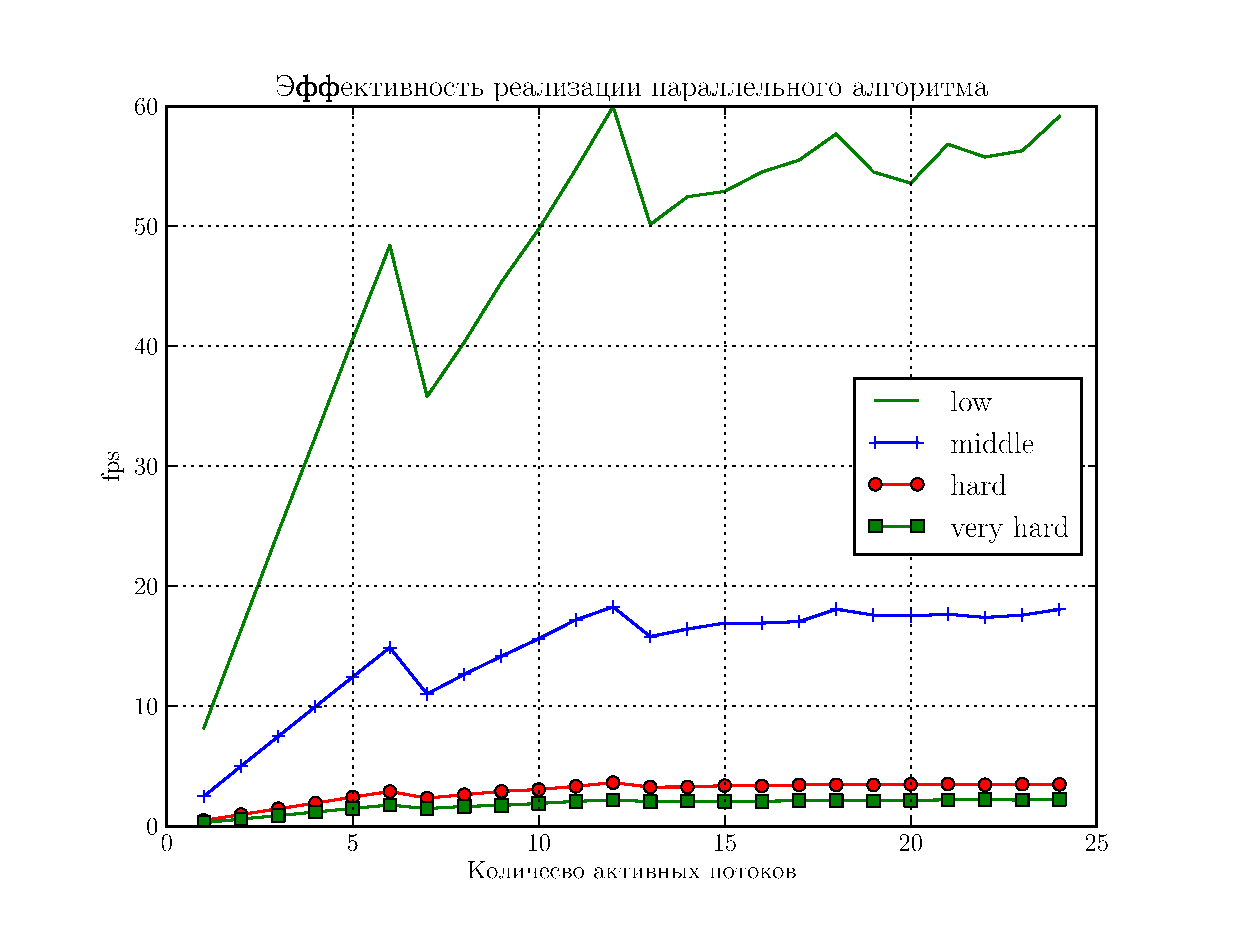
\includegraphics[width=\textwidth]{perf/table_perf.eps}
\caption{Производительность реализации параллельного алгоритма}\label{fig:perf_parallel_alg}
\end{figure}

\begin{figure}[H]
\centering
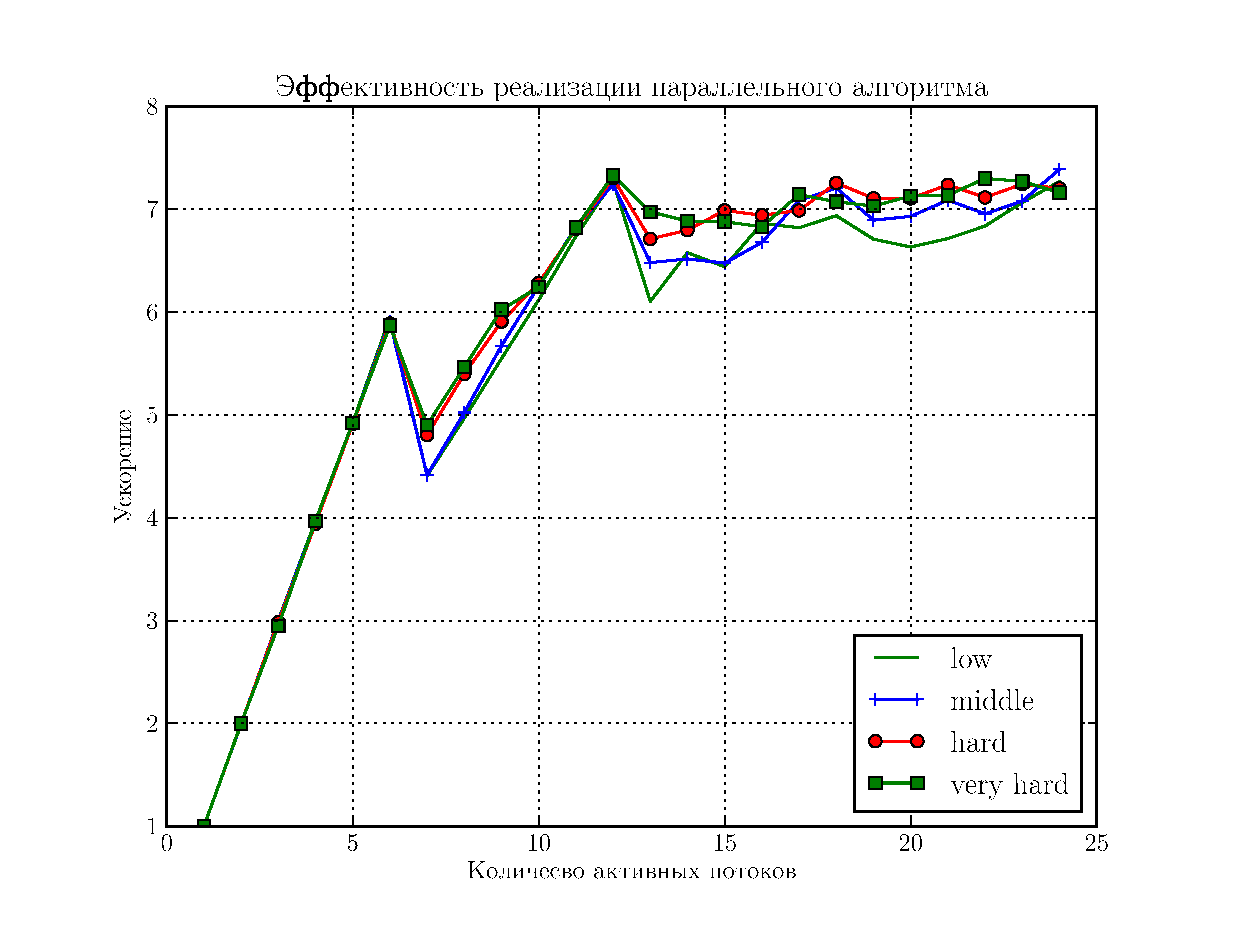
\includegraphics[width=\textwidth]{perf/table_perf_eff.eps}
\caption{Эффективность реализации параллельного алгоритма}\label{fig:eff_parallel_alg}
\end{figure}

\subsection{Наследование и полиморфизм}

Для более лучшего качества рендеринга было принято решение использовать несколько приметивов. Были реализованы следующие приметивы: плоскость, сфера, треугольник. Т.к. работа со всеми приметивами одинакова, то было реализован один базовый класс предок(Primitive), который представлял из себя интерфейс для реализации основных методов. Обработка происходила очевидным образом. 

Использование полиморфизма позволяет избежать использование информации о типе во время исполнения(RTTI) и сделать код более понятным и компакным. Или можно реализовывать каждый алгоритм с различными типами данных, но это очень сильно раздувает код.

При использование полиморфизма возникают накладные расходы связанные с тем, что при вызове операций у абстрактного класса, необходимо во время испонения определить, к какому классу принадлежит данный объект и вызвать соответствующий метод. 

\textbf{Описание теста}. Один базовый класс и 4 класса потомка, создаются в одном массиве. 
Затем циклом пробегаем и вызывает один метод у каждого элемента, тем самым получаем первое время.
Далее пробегаем по другому массиву, точно такой же длины и вызываем такой же метод у объекта, который не является ни чьим наследником - второе время.
Второе время принимаем за 100\% и оцениваем на сколько первое время больше второго. 

Оценим насколько велики накладные расходы в зависимости от размера массива.

\begin{figure}[H]
\centering
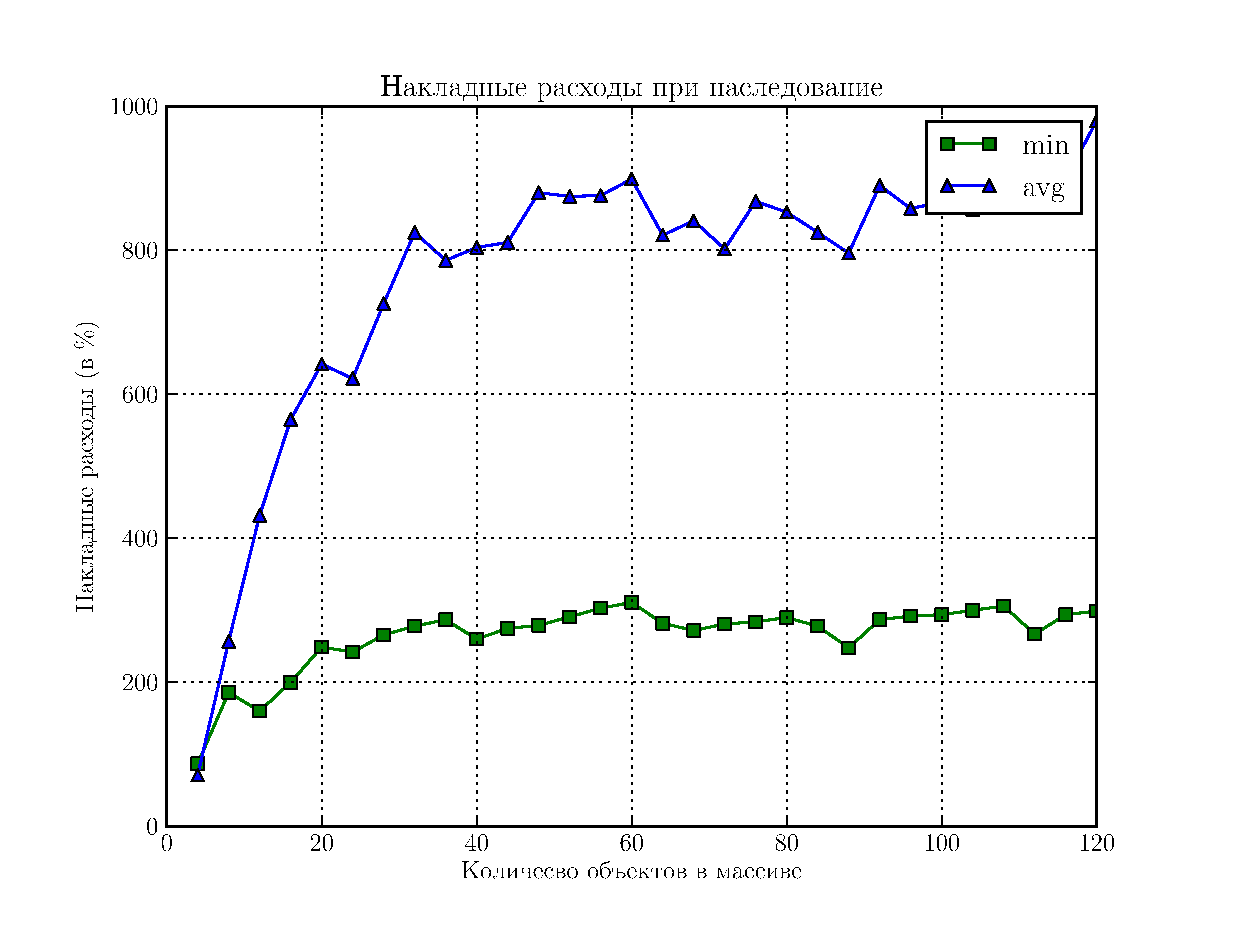
\includegraphics[width=\textwidth]{apps/compare_virtual_methods_l.eps}
\caption[Накладные расходы при наследование $\No$1]{Накладные расходы при наследование для малого количества объектов}\label{fig:compare_virtual_methods_1}
\end{figure}

Для массива, содержащего порядка сотни объектов, накладные расходы достаточно велики.

\begin{figure}[H]
\centering
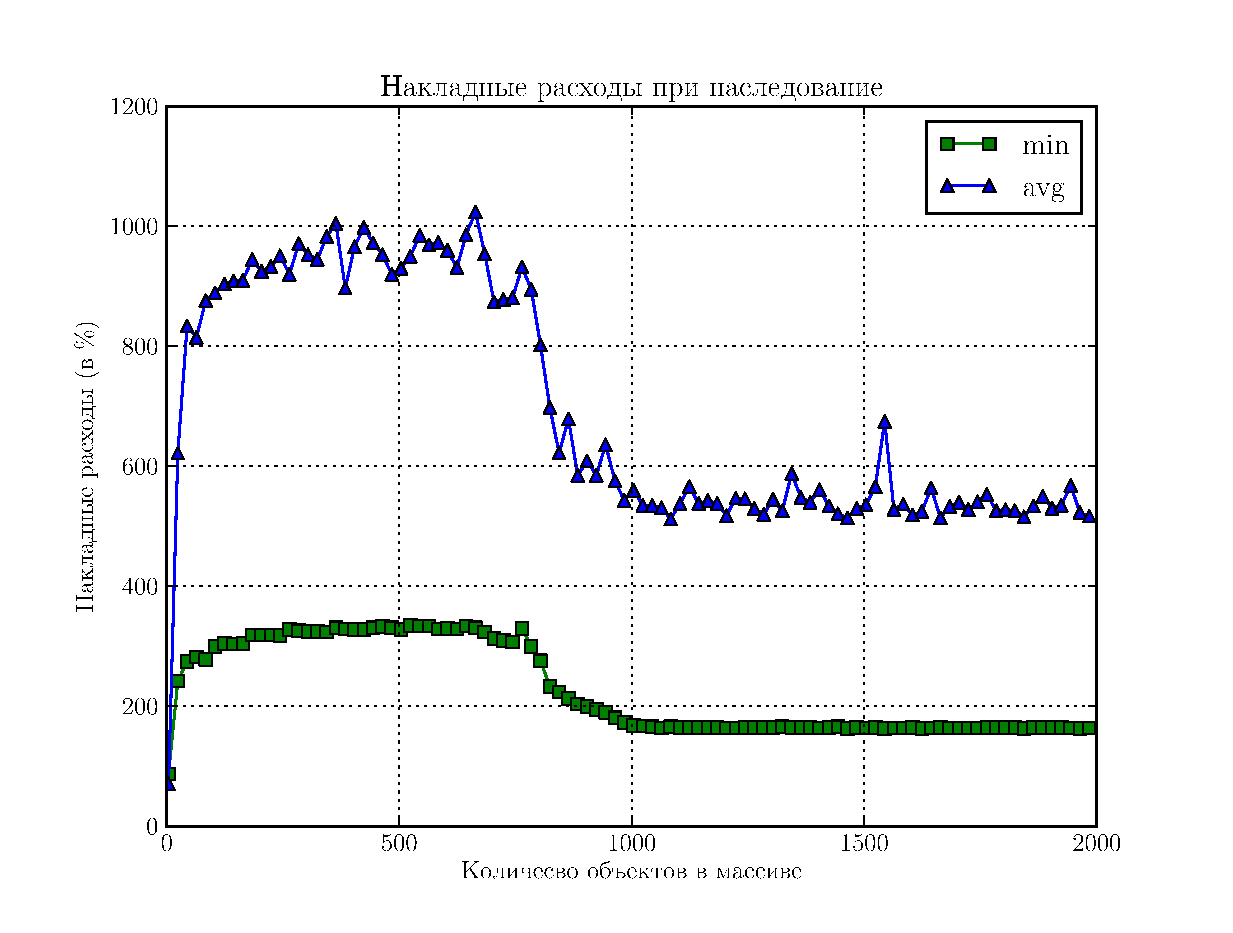
\includegraphics[width=\textwidth]{apps/compare_virtual_methods_b.eps}
\caption[Накладные расходы при наследование $\No$2]{Накладные расходы при наследование для большого количества объектов}\label{fig:compare_virtual_methods_2}
\end{figure}

\subsection{TBB vs OpenMP}

\subsection{Компилирование высокоуровнего кода в ассемблер}

Ассемблерные вставки, которые показывают что вычисление отражающего луча это одно SSE.

\subsection{Основные техники оптимизации программы}


%%%%%%%%%%%%%%%%%%%%%%%%%%%%%%%%%%%%%%%%%%%%%%%%%%%%%%%%%%%%%%%%%%%%%%%%%%%%%%%%%%%%%%%%%%%

\newpage
\section*{Заключение}
\addcontentsline{toc}{section}{Заключение} 
Задача трассировки лучей является по настоящему трудным испытанием для центрального процессора. Несмотря на то, что процессор обладает хорошей производительностью на ядро, общей производительности ему не хватает. Несмотря на столь малые мощности, удалось реализовать достаточно быстрый алгоритм на центральном процессоре. Для большей производительности была разработана эффективная параллельная версия программы с использованием библиотеки TBB и OpenMP. Благодаря использованию языка с++ и технике шаблонных выражений, удалось еще повысить производительность программы. Программа продемонстрировала хорошую производительность: используя всего лишь один процессор можно получать изображения в реальном времени.

%%%%%%%%%%%%%%%%%%%%%%%%%%%%%%%%%%%%%%%%%%%%%%%%%%%%%%%%%%%%%%%%%%%%%%%%%%%%%%%%%%%%%%%%%%%

\newpage
\begin{thebibliography}{99}
	\bibitem{morozov_kazan} Морозов А. С. Трассировка лучей в реальном времени на многоядерном процессоре. Высокопроизводительные параллельные вычисления на кластерных системах (HPC-2008). Материалы Восьмой Международной конференции-семинара. Казань, ноябрь 17-19, 2008. Труды конференции — Казань: Изд. КГТУ, 2008. - С. 241.
	\bibitem{morozov_microsoft} Морозов А. С. Высокопроизводительная реализация трассировки лучей с использованием Microsoft MPI. Технологии Microsoft в теории и практике программирования. Материалы конференции /Под ред. Проф. В.П. Гергеля. - Нижний Новгород: Изд-во Нижегородского госуниверситета, 2009. - 527 с.
	\bibitem{morozov_pavt} Морозов А. С. Сравнительный анализ алгоритма трассировки лучей на системах с общей и разделяемой памятью. Параллельные вычислительные технологии (ПаВТ’2009): Труды международной научной конференции (Нижний Новгород, 30 марта - 3 апреля 2009 г.). - Челябинск: Изд. ЮурГУ, 2009. - 839 с
	\bibitem{latex} Львовский С.М. Набор и верстка в системе \LaTeX. – 4-е изд., стереотипн. – М.: МЦНМО, 2006
	\bibitem{alloftex} Кнут, Дональд, Э. Все про \TeX. : Пер. с англ. --- М. : Издательский дом ''Вильямс'', 2003. --- 560 с. : ил. --- Парал. Тит. англ.
	\bibitem{inteloptimize} Гербер Р., Бик А., Смит К., Тиан К. Оптимизация ПО. Сборник рецептов. --- СПб.: Питер, 2010. --- 352 с.: ил. --- (Серия ''Библиотека программиста'').
	\bibitem{templatecpp} Вандевурд, Дэвид, Джосаттис, Николаи М. Шаблоны C++: справочник разработчика. : Пер. с англ. --- М. : Издательский дом ''Вильямс'', 2008. --- 544 с. : ил. --- парал. тит. англ.
	\bibitem{straustrupcpp} Б. Страуструп Язык программирования C++. Специальное издание / Пер. с англ. --- М.: ООО ''Бином-Пресс'', 2006. --- 1104 с.: ил.
	\bibitem{sivakov} Сиваков И. Как компьютер рассчитывает изображения. Технология программного рендеринга, 11.03.2004. \\ (\href{http://www.fcenter.ru/online.shtml?articles/hardware/videos/8749}{http://www.fcenter.ru/online.shtml?articles/hardware/videos/8749})
	\bibitem{biovulf} Дмитрий Мороз. "Беовульф": Создание фильма, 11.12.2007.\\ (\href{http://www.3dnews.ru/editorial/beowulf}{http://www.3dnews.ru/editorial/beowulf})
	\bibitem{intelintrinsic} Intel® C++ Intrinsics Reference \\ (\href{http://www.intel.com/products/processor/manuals/}{http://www.intel.com/products/processor/manuals/})
	\bibitem{intelmanual} Intel 64 and IA-32.Architectures Software Developer's Manual \\ (\href{http://www.intel.com/products/processor/manuals/}{http://www.intel.com/products/processor/manuals/})
	\bibitem{tbbtutor} Intel® Threading Building Blocks. Tutorial \\ (\href{http://www.threadingbuildingblocks.org/}{http://www.threadingbuildingblocks.org/})
	\bibitem{tbbmanual} Intel® Threading Building Blocks. Reference Manual \\ (\href{http://www.threadingbuildingblocks.org/}{http://www.threadingbuildingblocks.org/})
	\bibitem{cppexpressiontemplate} C++ Expression Templates An Introduction to the Principles of Expression Templates, 2003 \\ (\href{http://www.angelikalanger.com/Articles/Cuj/ExpressionTemplates/ExpressionTemplates.htm}{http://www.angelikalanger.com/.../ExpressionTemplates.htm})
	\bibitem{intelcore980x} Шесть ядер для десктопа: Intel Core i7-980X Extreme Edition, 07.04.2010 \\ (\href{http://www.fcenter.ru/online.shtml?articles/hardware/processors/28480}{\small http://www.fcenter.ru/online.shtml?articles/hardware/processors/28480})
	\bibitem{rdtscp} How to Benchmark Code Execution Times on Intel IA-32 and IA-64 Instruction Set Architectures. September 2010
	\bibitem{pahomov} Сергей Пахомов. Тестируем Prescott \\ (\href{http://www.compress.ru/article.aspx?id=10204&iid=421}{\small http://www.compress.ru/article.aspx?id=10204\&iid=421})
	\bibitem{perf_core_i7}\href{http://techgage.com/print/intels_core_i7-980x_extreme_edition_-_ready_for_sick_scores}{\small http://techgage.com/print/intels\_core\_i7-980x\_extreme\_edition\_-\_ready\_for\_sick\_scores}
	\bibitem{perf_radeon6990}\href{http://techreport.com/articles.x/20537}{\small http://techreport.com/articles.x/20537}
\end{thebibliography}

\newpage
\listoffigures

\newpage
\listoftables

\newpage
\documentclass[12pt, a4paper]{article}
\usepackage[utf8]{inputenc}
\usepackage[russian]{babel} 
\usepackage[T2A]{fontenc}
\usepackage[pdftex]{graphicx}
\usepackage{amstext}
\usepackage{textcomp}
\usepackage{multicol}
\usepackage{hyperref}
\usepackage{setspace}
\usepackage[usenames,dvipsnames]{color} % для source-highlight
\usepackage{indentfirst}

% меняем размеры страницы
\usepackage{geometry}
\geometry{left=2.5cm}
\geometry{right=2.0cm}
\geometry{top=1.5cm}
\geometry{bottom=2.5cm}

% шрифты
%\defaultfontfeatures{Scale=MatchLowercase}
%\setmainfont[SmallCapsFont={* Caps}]{Liberation Serif}
%\usepackage{xltxtra}
%\setmainfont[Mapping=tex-text]{Linux Libertine O}
%\setmonofont[SmallCapsFont={Courier New}]{Courier New}
%\fontsize{10}{10}


%\usepackage{courier}
%\setmainfont[Mapping=tex-text]{Courier}


% изменение межстрочного интервала
\def\heightline{1.2}
\linespread{\heightline} % 1.3 - это полуторный

%%%%%%%%%%%%%%%%%%%%%%%%%%%%%%%%%%%%%%%%%%%%%%%%
%%% добавляем точки в Оглавление

\renewcommand{\thesection}{\arabic{section}.} 
\renewcommand{\thesubsection}{\arabic{section}.\arabic{subsection}.} 
\renewcommand{\thesubsubsection}{\arabic{section}.\arabic{subsection}.\arabic{subsubsection}.} 

%%%%%%%%%%%%%%%%%%%%%%%%%%%%%%%%%%%%%%%%%%%%%%%%

% определим новые команды
\def\VEC#1#2#3{\left( \begin{array}{c} #1 \\ #2 \\ #3 \end{array} \right) }
\def\VECXYZ#1{\left( \begin{array}{c} x_#1 \\ y_#1 \\ z_#1 \end{array} \right) }

\newcommand{\HRule}{\noindent\rule{\linewidth}{0.45mm}}

\newcounter{sourcecode}
\setcounter{sourcecode}{1}
\newcommand*{\cppsource}[2]{\par{\HRule \small \tt \bf \noindent \ Листинг \arabic{sourcecode}. {\rm \small #2} \vspace{0.25cm}}%
\addtocounter{sourcecode}{1} \input{#1} \HRule}

\makeindex

\begin{document}

\begin{titlepage}
\begin{center}
{\large Федеральное агентство по образованию Российской Федерации\\
\vspace{0.25em}
Государственное образовательное учреждение\\высшего профессионального образования\\Нижегородский государственный университет им. Н.И. Лобачевского\\
\vspace{0.25em}
Факультет вычислительной математики и кибернетики\\
\vspace{0.25em}
Кафедра математического обеспечения ЭВМ\\
\vspace{3em}
Дипломная работа\\
}
\vspace{1em}
{\bf \huge
	\textsf{ Трассировка лучей в реальном времени на x64~архитектуре \\ } 
}
\end{center}
\vspace{0.5cm}
\begin{multicols}{2}
\large 
\noindent 
Работа допущена к защите \\
Заведующий кафедрой МО ЭВМ \\
д.ф.--м.н., проф. \\

\vspace*{1em}
{ \noindent
\hspace*{1.5cm}\hbox to 0cm{\raisebox{-1em}{\small Подпись}}\hspace{-1.5cm}{\hrulefill\ Стронгин Р. Г. }
}

\vspace*{1.0em}
{ \noindent
\hbox to 0cm{\raisebox{0.25em}{<<\ \ \ \ \ \  >>}}{\hrulefill\ 2011 г. }
}
\vbox to 5 cm{\ }
Исполнитель: \\
студент 2 курса магистратуры \\
факультета ВМК группы 86М1 \\

\vspace*{1em}
{ \noindent
\hspace*{1.5cm}\hbox to 0cm{\raisebox{-1em}{\small Подпись}}\hspace{-1.5cm}{\hrulefill\ Морозов А. С. }
}

\vspace*{1.0em}
{ \noindent
\hbox to 0cm{\raisebox{0.25em}{<<\ \ \ \ \ \  >>}}{\hrulefill\ 2011 г. }
}
\\
Научный руководитель: д. т. н., \\
профессор кафедры МО ЭВМ \\

\vspace*{1em}
{ \noindent
\hspace*{1.5cm}\hbox to 0cm{\raisebox{-1em}{\small Подпись}}\hspace{-1.5cm}{\hrulefill\ Турлапов В. Е. }
}

\vspace*{1.0em}
{ \noindent\newcommand{\z}{\textbf{Задача. }}
\hbox to 0cm{\raisebox{0.25em}{<<\ \ \ \ \ \  >>}}{\hrulefill\ 2011 г. }
}
\end{multicols}

\vfill 
\begin{center} 
{\rm \large Нижний Новгород \\ 2011 г.} 
\end {center} 
\end{titlepage} 

\tableofcontents

\newpage
\section*{Введение}
\addcontentsline{toc}{section}{Введение} 
В кино индустрии к современной компьютерной графике предъявляются серьезные требования физически корректного моделирования о освещения сцен, состоящая из множества примитивов с различными характеристиками взаимодействия со светом. Даже малейшие неточности, могут отбросить художественный или анимационный фильм в рубрику любительского кино, и при этом не принести ожидаемой прибыли. Особенные требования предъявляются именно к художественному фильму, т. к. используемые спец эффекты должны выглядеть настолько реалистично, что бы зритель не смог различить, где настоящий актер, а где рисованный двойник. Используя только физически правильные модели и алгоритмы можно обеспечить растущую потребность в более реалистичной трехмерной графике. \par
   С каждым новым фильмом, каждый из нас видит прогресс в компьютерной графике. Картинка становится все красочнее и правдоподобнее, но это все не дается просто так. Естественно, платить за это приходится высокой вычислительной трудоемкостью расчетов. Несомненно, что с каждым годом производительность вычислительной техники растет, но она сразу же «расходуются» на новые спецэффекты. Существует наблюдение, которое гласит, что время расчета одного кадра не изменяется. Среднее время расчета полного фильма 15 лет назад занимал около 10-12 месяцев, так и сегодня тратят столько же времени, хотя при этом, надо заметить, что производительность современных компьютеров в десятки, а то и в сотни раз превышает производительность компьютеров того времени. Со временем улучшается и требования к самому изображению. Если несколько лет
назад картинка с разрешением 1024х768 считалась излишеством в компьютерной графики, то уже сейчас это слишком мало и все считают де факто FullHD\footnote{ \index{FullHD}FullHD -- это разрешение экрана 1920х1080 пикселей} , хотя уже задумываются о еще лучшем качестве. В последний год компьютерная индустрия, дабы не потерять зрителя, начала использовать новые технологии — 3D, которая требует еще большей вычислительной мощности. \par
   Именно за последние несколько лет компьютеры стали по настоящему параллельными. Появились многоядерные процессоры. И именно по этому, что 15 лет назад было трудоемкой задачей рендеринга, то сейчас это можно получить почти в реальном времени при том же качестве результата.

\newpage 
\section{Постановка задачи}
Главной целью данной работы является разработка и исследование алгоритма трассировки лучей на архитектуре x64 с применением ускоряющей структуры. Для решения главной задачи, требуется решить ряд следующих подзадач:
\begin{itemize}
	\item Реализовать высокопроизводительный алгоритм трассировки лучей на центральном процессоре
	\item Реализация и исследование оптимизированной версии с использованием векторных расширений архитектуры x64
	\item Реализация и исследование специализированного класса векторов для алгоритма трассировки лучей основанного на технологии шаблонных выражений, с применением векторных оптимизаций  - \index{SIMD}SIMD\footnote{ Single Instruction, Multiple Data — Одна Инструкция, Много Данных } инструкции 
	\item Реализация параллельной версии алгоритма трассировки лучей с использованием OpenMP, TBB
	\item Сравнение параллельной версии алгоритма трассировки лучей с использованием библиотеки TBB и расширения языка OpenMP
	\item Реализация ускоряющей структуры
	\item Сравнение реализации алгоритма с использованием ускоряющей структуры и без нее
\end{itemize}
   В качестве основного языка программирования выбирается язык С++, а для отображения результатов — кроссплатформенная библиотека SDL. 
   
\newpage 
\section{Архитектура центрального процессора}
\subsection{Архитектура процессоров семейства x86}
Рассмотрим основные архитектурные особенности центрального процессора.
Одни из базовых понятий для производительности процессора:
\begin{itemize}
	\item Latency (Латентность команды) --- это число тактов, необходимое для завершения одной команды с момента готовности входных данных команды(выборки их из памяти) и начало ее выполнения
	\item Throughput (Пропускная способность команды) --- это число тактов ожидания, которое требуется процессору перед запуском на выполнение такой же команды
\end{itemize}   

\subsection{Архитектура процессоров семейства x64}
\subsubsection{Архитектура процессора Intel Core i7 980X}
\noindent{\bf\ttОбзор}\\
Intel Core i7 — семейство процессоров x86-64 Intel. Core i7 980X это процессор семейства Gulftown вышедшего в 2010 году. Основные характеристики представлены с помощью программы cpu-z:
\begin{center}
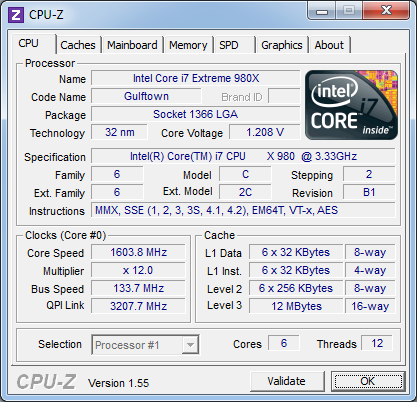
\includegraphics[scale=1]{imgs/cpu-z.png} 
\end{center}

%%%%%%%%%%%%%%%%%%%%%%%%%%%%%%%%%%%%%%%%%%%%%%%%%%%%%%%%%%%%%%%%

\newpage
\section{Трассировка лучей}
Классический ray tracing~[\cite{sivakov}], или метод трассировки лучей, предложен Артуром Аппелем (Arthur Appel) еще аж в 1968 году и дополнен алгоритмом общей рекурсии, разработанным Whitted в 1980 году. Понадобилось почти 12 лет эволюции вычислительных систем, прежде чем этот алгоритм стал доступен для широкого применения в практических приложениях. Реализация высокопроизводительной версии трассировки лучей уже предпринимаются различными компаниями. О сложности задачи трассировки лучей можно прочитать в соответствующих источниках~[\cite{biovulf}].

\subsection{Алгоритмы трассировки лучей}
Суть метода заключается в отслеживании траекторий лучей и расчета взаимодействий с лежащими на траекториях объектами, от момента испускания лучей источником света до момента попадания в камеру. Под взаимодействием луча с объектами понимаются процессы диффузного (в смысле модели локальной освещенности), многократного зеркального отражения от их поверхности и прохождение лучей сквозь прозрачные объекты. Таким образом, ray tracing – первый метод расчета глобального освещения, рассматривающий освещение, затенение (расчет тени), многократные отражения и преломления. Различают два основных вида метода трассировки лучей: \textbf{\textit{прямой}} -- \index{forward ray tracing}forward ray tracing, и \textbf{\textit{обратный}} -- \index{backward ray tracing}backward ray tracing.

\subsubsection{Прямой метод трассировки лучей}
В прямом методе траектории лучей строятся от источника ко всем точкам всех объектов сцены (первичные лучи). Затем проверяется ориентация каждой точки относительно источника, и, если она лежит на стороне объекта, обращенной в противоположную от источника сторону, точка из расчетов освещенности исключается. Для всех остальных точек вычисляется освещенность с помощью локальной модели освещения. Если объект не является отражающим или прозрачным, то есть поверхность объекта только диффузно рассеивает свет, траектория луча на этой точке обрывается (заканчивается). Если же поверхность объекта обладает свойством отражения (\index{reflection}reflection) и/или преломления (\index{refraction}refraction), из точки строятся новые лучи, направления которых совершенно точно определяются законами отражения и преломления.
\par
    Для построенных таким образом траекторий новых лучей может быть только три исхода. Луч либо выходит за пределы видимой из камеры области сцены, в этом случае все проделанные для него до этого момента расчеты освещенности отбрасываются, поскольку они не принимают участия в формировании изображения. Или луч попадает в камеру, тогда рассчитанная освещенность формирует цвет соответствующего пиксела изображения. Или луч встречает на своем пути новый
объект, тогда для новой точки пересечения повторяется расчет освещенности и построения лучей отражения и преломления в зависимости от свойств поверхности объекта (рекурсия). Построение новых траекторий и расчеты ведутся до тех пор, пока все лучи либо попадут в камеру, либо выйдут за пределы видимой области. Очевидно, что при прямой трассировке лучей мы вынуждены выполнять расчеты для лучей, которые не попадут в камеру, то есть, проделывать бесполезную работу. По некоторым оценочным данным доля таких "слепых"лучей довольно велика. Эта главная, хотя и далеко не единственная, причина того, что метод прямой трассировки лучей считается неэффективным и на практике не используется(в чистом виде).

\subsubsection{Обратный метод трассировки лучей}
Обратной метод трассировки лучей, или backward ray tracing. Этот метод расчетов основывается на построении лучей от наблюдателя через плоскость экрана вглубь сцены, а не от источника, то есть -- наоборот. Этот способ достаточно изящен, что позволяет решить массу проблем, возникающих при прямой трассировке, а сам метод отличается простотой и понятностью. Лучи теперь строятся иначе. А именно, по двум точкам: первая точка, общая для всех лучей – положение камеры (наблюдателя), вторая точка определяется положением пиксела на плоскости видового окна. Таким образом, направление каждого луча строго определено (две точки в пространстве определяют одну и только одну прямую – школьный курс геометрии), и количество первичных лучей также известно – это общее количество пикселей видового окна. Например, если видовое окно имеет 1920 пикселей по ширине и 1200 пикселей по высоте, количество лучей составит 1920 х 1200 = 2 304 000. Каждый луч
вдоль заданного направления продлевается от наблюдателя вглубь трехмерной сцены, и для каждой траектории выполняется проверка на пересечение со всеми объектами сцены и с отсекающими плоскостями. Если пересечений с объектами нет, а есть пересечение только с плоскостью отсечения, значит луч выходит за пределы видимой части сцены, и соответствующему пикселю видового окна присваивается цвет фона. Если луч пересекается с объектами сцены, то среди всех объектов выбирается тот, который ближе всего к наблюдателю. В точке пересечения с таким объектом строится три новых, так называемых вторичных луча. \par

\begin{center}
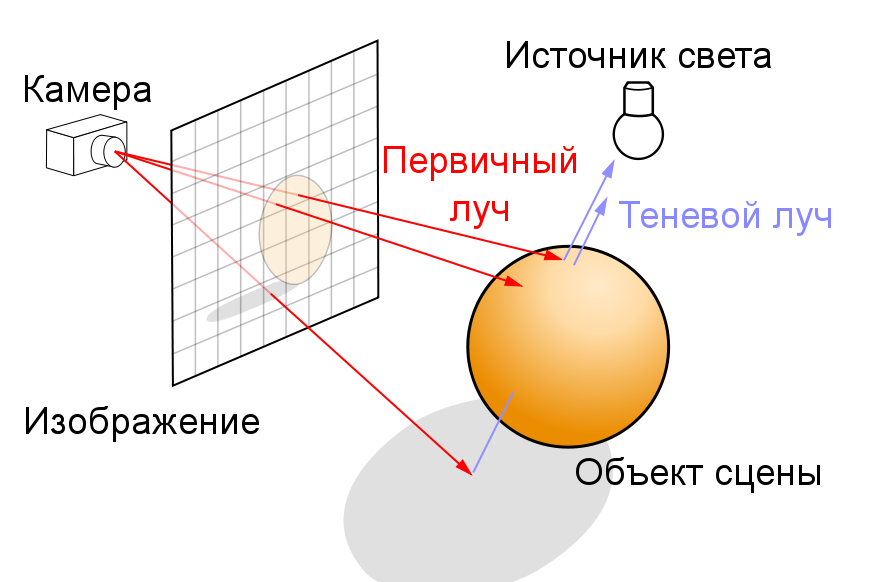
\includegraphics[scale=0.5]{imgs/Ray_trace_diagram_rus.png} 
\end{center}

Первый луч строится в направлении источника света. Если источников несколько, строится несколько таких лучей, по одному на каждый источник. Основное назначение этого луча – определить ориентацию точки (обращена точка к источнику или от него), наличие объектов, закрывающих точку от источника света, и расстояние до источника света. Если точка обращена в противоположную сторону от источника света или закрыта другим непрозрачным объектом, освещенность от такого источника не рассчитывается, точка находится в тени. В случае затеняющего прозрачного объекта интенсивность освещения уменьшается в соответствии со степенью прозрачности. Если точка закрыта от освещения всеми источниками сцены, ей присваивается фоновый (\index{ambient или фоновый цвет}ambient) цвет. В противном случае точка освещена, интенсивность и цвет освещения рассчитываются при помощи локальной модели освещенности, как сумма освещенностей от всех источников, для которых эта точка не закрыта другими объектами. Этот тип луча получил название \index{shadow ray или теневой луч} \textit{\textbf{shadow ray}} (иногда его еще называют \index{illumination ray}illumination ray) – теневой луч. Если поверхность объекта не является отражающей и непрозрачна, теневой луч – единственный тип лучей который строится, траектория первичного луча обрывается (заканчивается), и дальнейшие расчеты не выполняются. Рассчитанный цвет (освещенности или тени) присваивается тому пикселю видового окна, через который проходит соответствующий первичный луч.
   \par
   Второй луч строится, если поверхность объекта обладает отражающими свойствами, и называется \index{reflection ray или отраженный луч} reflection ray, или луч отражения. Направление отраженного луча определяется по закону:
$$
	\vec{R} = \vec{I} - 2 \cdot \vec{N} (\vec{N} , \vec{I})
$$
где $\vec{R}$ - отраженный луч, $\vec{I}$ - падающий пераичный луч, $\vec{N}$ - нормаль к поверхности в точке соударения.
Для отраженного луча проверяется возможность пересечения с другими объектами сцены. Если пересечений нет, то интенсивность и цвет отраженного луча равна интенсивности и цвету фона. Если пересечение есть, то в новой точке снова строится три типа лучей – теневые, отражения и преломления.
Третий луч строится, если поверхность объекта прозрачна, и носит название \index{transparency ray или преломленный луч}transparency ray, т. е. луч преломленный. Направление для преломленного луча определяется следующим образом:
$$
 \vec{T} = \frac{n_1}{n_2} \cdot \vec{I} - \left[ \cos \alpha + \frac{n_1}{n_2} \cdot \left(\vec{N},\vec{I} \ \right) \right] \cdot \vec{N}
$$
$$
\cos \alpha = \sqrt{1 - \left( \frac{n_1}{n_2} \right) ^2 \cdot \left(1-\left(\vec{N},\vec{I}\ \right)^2\right)}
$$
где $\vec{T}$ - переломленный луч, $n_1$ - коэффициент рефракции для первой среды ( в которой растространяется первичный луч ), $n_2$ - коэффициент рефракции для второй среды прозрачного объекта.

Так же, как и в предыдущем случае, проверяется пересечение вновь построенного луча с объектами, и, если они есть, в новой точке строятся три луча, если нет -- используется интенсивность и цвет фона.

Таким образом, для каждого первичного луча можно построить древовидную структуру. Если древовидная структура для данного луча построена, то расчет освещенности можно выполнить в следующем порядке. Для каждой ветви дерева спускаемся вдоль древовидной структуры к последнему пересечению вторичного луча и поверхности (будем дальше называть их узлами). Поскольку это последний узел в цепи, то  вкладов от преломлений и отражений нет, поэтому, освещенность узла вычисляется при помощи локальной модели освещения с учетом видимости источников света для данного узла. Затем, вычисленная освещенность передается вверх по ветви к следующему ближайшему узлу. Освещенность в этом узле будет вычисляться по формуле:

$$
 \vec{I}_{total} = \vec{I}_{local} + K_{reflection} \cdot \vec{I}_{reflection} + K_{refraction} \cdot \vec{I}_{refraction}
$$

где $\vec{I}_{total}$ - полная освещенность в точке, $\vec{I}_{local}$ - локальная освещенность в точке, вычисленная от источников освещения с помощью одной из локальной модели освещенности, $K_{reflection}$ - коэффициент, определяющий отражающие свойства поверхности, $\vec{I}_{reflection}$ - освещенность предыдущей точки, переданная вдоль ветки отражения,   $K_{refraction}$ - коэффициент, определяющий преломляющие свойства поверхности $\vec{I}_{refraction}$ - освещенность предыдущей точки, переданная вдоль ветки преломления

Естественным завершением трассировки лучей является выход всех испущенных вторичных лучей за пределы видимой области и их рассеяние на чисто диффузных объектах. Результат вычислений будет наиболее точным. Но, если сцена достаточно сложна, такой расчет будет очень медленным, а в некоторых случаях и невозможным по причине ограниченности аппаратных ресурсов. Легко увидеть, что вклад освещенности от каждого нового вторичного луча очень быстро уменьшается по той простой причине, что коэффициенты свойств отражения и преломления материалов меньше единицы. Поэтому часто трассировку лучей прекращают, когда вклад от следующего узла ветви становится меньше заданной величины. Это также достаточно точный метод расчетов, который может быть использован для получения качественных результатов при определенных условиях. Наконец, для получения оценочного расчета можно оборвать трассировку лучей после выполнения заданного количества итераций, это самый быстрый и наименее точный расчет.

\subsubsection{Достоинства и недостатки}

Основные достоинства рекурсивного метода обратной трассировки лучей – расчет теней, многократных отражений и преломлений, значительно повысивших степень реалистичности получаемых изображений.
Основные недостатки: неучет вторичного освещения от диффузно отраженного объектами света; низкая скорость и высокая вычислительная стоимость расчетов – в классическом рейтресинге необходимо проверять на пересечение каждый луч со всеми объектами сцены, в результате от 70 до 95 процентов всего времени расчетов тратится на вычисление пересечений; резкие границы цветовых переходов тени/подсветок/прозрачности; \index{aliasing}aliasing – "зазубренность" линий и т. д.; дискретность определяющих цвет пиксела первичных лучей – одного первичного луча недостаточно для корректного определения цвета пиксела, формирующего изображение.


\subsection{Модели освещения}

В соответствии с принятым в компьютерной графике подходом, расчет освещенности распадается на две основные задачи. Первая – определить способ расчета освещенности в произвольной точке трехмерного пространства, решается при помощи построения обобщенной математической модели освещенности (Illuminating model). Вторая задача – применение Illuminating model для компьютерных расчетов освещенности трехмерных объектов с конкретной геометрией и свойствами поверхности, решается при помощи так называемой модели затенения (Shading model).

Моделей освещенности к настоящему моменту разработано несколько. Самая первая,и самая простая – локальная модель освещенности. Эта модель не рассматривает процессы светового взаимодействия объектов сцены между собой, а только расчет освещенности самих объектов. Вторая, глобальная модель освещенности – Global Illuminations, рассматривает трехмерную сцену как единую систему и пытается описывать освещение с учетом взаимного влияния объектов. В рамках этой модели рассматриваются такие вопросы, как многократное отражение и преломление света (ray tracing), рассеянное освещение (radiosity), каустик(caustic) и фотонные карты (photon mapping) и другие. 

\subsubsection{Глобальные модели освещения}

Глобальное освещение (global illumination) — это название ряда алгоритмов, используемых в 3D-графике, которые предназначены для добавления более реалистичного освещения в трёхмерные сцены. Такие алгоритмы учитывают не только свет, который поступает непосредственно от источника света (прямое освещение, англ. direct illumination), но и такие случаи, в которых лучи света от одного и того же источника, отражаются на других поверхностях сцены (непрямая освещенность, англ. indirect illumination).

Теоретически отражение, преломление, тень — примеры глобального освещения, потому что, для их имитации необходимо учитывать влияние одного объекта на другие (в отличие от случая когда на объект падает прямой свет). На практике, однако, только моделирование диффузного отражения или каустики называется глобальным освещением.

Изображения полученные в результате применения алгоритмов глобального освещения часто кажутся более фотореалистичными, чем те, в процессе рендеринга которых применялись алгоритмы только прямого освещения, но для просчета глобального освещения требуется гораздо больше времени.

\subsubsection{Локальные модели освещения}

Существующие локальные модели освещения можно разделить на две категории. К первой категории относятся эмпирические модели. Они обычно эффективны в плане быстродействия и некоторые из них дают довольно реалистичную картинку. Они обычно не оперируют такими физическими величинами, как световая энергия, или световой поток. Однако эти модели находят довольно широкое применение в областях, где не требуется точная физическая информация об освещении (например, спецэффекты в фильмах, программы для художников и дизайнеров, для рекламных целей)

Ко второй категории относятся модели, базирующиеся на физических представлениях о теории света. Изображения, полученные с использованием этих моделей, очень хорошо соотносятся с экспериментальными данными. Поэтому эти модели находят применение там, где важна точная имитация поведения света (оформление интерьеров, архитектура)

\subsubsection{Модель Фонга}

Это эмпирическая модель. В самом общем случае, в свете требования фотореалистичности, эта модель учитывает и неявное ambient-освещение. Ambient-освещение, или его еще называют фоновым (background), – это окружающее объект освещение от удаленных источников, чье положение и характеристики не известны. Необходимость учета ambient-освещения, пусть и очень грубо, обусловлена тем, что его вклад может быть достаточно велик – до 50\% от общей освещенности. В Local Illumination считают, что фоновое освещение задает цвет (и его интенсивность) объекта в отсутствии явных источников света или в тени. Не несет никакой информации об объекте, кроме значения простого цвета, равномерно заливающего контур объекта.

Интенсивность такого освещения постоянна и равномерно распределена во всем пространстве, расчет его отражения поверхностью выполняется по формуле:

$$
 \vec{I}_{amb} = K_{a} \cdot \vec{I}_{a}
$$

где $\vec{I}_{amb}$  - интенсивность отраженного ambient освещения, $K_{a}$ - коэффициент, характеризующий отражающие свойства поверхности для  ambient-освещения, $\vec{I}_{a}$ - исходная интенсивность ambient-света, падающего на поверхность.

Часть света от прямых источников зеркально отражается поверхностью, а остальной свет диффузно рассеивается во всех направлениях. Кроме чисто зеркального отражения, которое имеют идеально отполированные поверхности, различают так называемое glossiness или распределенное зеркальное отражение – отражение в некотором створе углов, а не на один единственный угол. Такое рассеяние света обусловлено микрорельефом ("шероховатостью") поверхности, то есть поверхность реальных объектов не является идеально гладкой, а состоит из большого количества микровыступов и впадин, которые зеркально отражают падающий свет под разными углами. Результатом glossy-отражения является specular highlight – яркий световой блик, имеющий размер в зависимости от степени шероховатости поверхности. 

Интенсивность рассеянного света зависит от угла падающего на поверхность света по закону Ламберта (Lambert):

$$
 \vec{I}_{diff} = K_{diff} \cdot \vec{I}_{d} \cdot \cos(\alpha)
$$
 
где $\vec{I}_{d}$ - интенсивность падающего на поверхность света, $K_{diff}$ - коэффициент, характеризующий рассеивающие свойства поверхности, $\cos(\alpha)$ - угол между направлением на источник света и нормалью поверхности

Другими словами, поверхность будет освещена больше, если свет падает на нее перпендикулярно ($\alpha = 0$), и меньше, если свет падает под любым другим углом, поскольку в этом случае увеличивается освещаемая площадь. Диффузно рассеянный свет является главным источником визуальной информации о геометрии трехмерных объектов.

Как было уже сказано ранее, свет отражается зеркально в некотором створе углов, и для большинства реальных материалов мы всегда видим зеркальную подсветку в форме светового пятна, а не в форме яркой точки. Поэтому, для расчета интенсивности зеркально отраженного света используется формула, предложенная Фонгом:

$$
 \vec{I}_{spec} = K_{spec} \cdot \vec{I}_{s} \cdot \cos^n(\beta)
$$

где $\vec{I}_{spec}$ - интенсивность зеркально отраженного света,  $\vec{I}_{s}$ - интенсивность источника света,  $\vec{K}_{s}$ - коэффициент, характеризующий свойства зеркального отражения поверхности
$\beta$ - угол между направлением идеального отражения и направлением на наблюдателя, степень $n$ определяет размер пятна светового блика, чем больше $n$, тем меньше световой блик, и тем ближе отражающие свойства поверхности к свойствам идеального зеркала.

Формула Фонга – пример компьютерной фикции, поскольку она не имеет физического смысла. Ее используют просто потому, что она дает хорошие практические результаты. 

Таким образом, локальная модель освещенности предполагает расчет отраженной фоновой освещенности, диффузного и зеркального отражения от прямых источников: 

$$
 \vec{I}_{local} =  K_{amb} \cdot \vec{I}_{amb} +  K_{diff} \cdot \vec{I}_{diff} \cdot \left( \vec{L},\vec{N} \right) + K_{spec} \cdot \vec{I}_{spec} \cdot \left( \vec{R},\vec{V} \right)^n
$$



\subsection{Примитивы}
\subsubsection{\index{Плоскость}Плоскость}
Для определения пресечения луча с плоскостью, необходимо найти точку в пространстве, которая будет удовлетворять двум уравнениям: уравнению луча и уравнению плоскости.
\par
Уравнение луча:
\begin{equation}
\left\{
\begin{array}{ccccc}
x & = & x_0 & + & t \cdot x_d \\
y & = & y_0 & + & t \cdot y_d \\
z & = & z_0 & + & t \cdot z_d \\
\end{array}
\right.
\label{equation_ray}
\end{equation}
или
$$
\vec{R}(t) = \vec{O} + t \cdot \vec{D}
$$
где $O = \VECXYZ{0} $ - начало луча, а $D = \VECXYZ{d} $ - направление луча. 
\par
Уравнение плоскости задается следующим образом:
\begin{equation}
Ax + By + Cz + D = 0
\label{equation_plane}
\end{equation}
\par
Для того, что бы найти точку пересечения луча с плоскостью, необходимо подставить уравнение (\ref{equation_ray}) в (\ref{equation_plane}):
$$
A(x_0 + t \cdot x_d) + B(y_0 + t \cdot y_d) + C(z_0 + t \cdot z_d) + D = 0
$$
Раскроем скобки и приведем подобные
$$
t(Ax_d + By_d + Cz_d ) + Ax_0 + By_0 + Cz_0 + D = 0
$$
найдем неизвестную величину t
$$
 t = - \frac{Ax_0 + By_0 + Cz_0 + D}{Ax_d + By_d + Cz_d}
$$
из уравнения видно, что луч либо пересекает плоскость в какой то точке, либо нет. Это связано с тем, что если $Ax_d + By_d + Cz_d = 0$, то плоскость и луч параллельны друг другу. Т.к. $P = \VEC{A}{B}{C} $ - это нормаль к поверхности, то из геометрии известно, что если $( D , P ) = 0$, то вектора параллельны.
\par
   Для того, что бы найти величину $t$, необходимо рассчитать всего несколько скалярных произведений:
$$
t = - \frac{(O, P) + D}{(D, P)}
$$
при условии, что $(D, P) \neq 0$

\subsubsection{\index{Сфера}Сфера}
Для сферы необходимо проделать те же выкладки.
Уравнение луча:
\begin{equation}
\left\{
\begin{array}{ccccc}
x & = & x_0 & + & t \cdot x_d \\
y & = & y_0 & + & t \cdot y_d \\
z & = & z_0 & + & t \cdot z_d \\
\end{array}
\right.
\label{equation_ray}
\end{equation}
или
$$
\vec{R}(t) = \vec{O} + t \cdot \vec{D}
$$
Уравнение сферы записывается следующем образом:
\begin{equation}
(x-x_c)^2 + (y-y_c)^2 + (z-z_c)^2 = r^2
\label{equation_sphere}
\end{equation}
где $S = \VECXYZ{c}$ - центр сферы, а $r$ - радиус. Подставим уравнение (\ref{equation_ray}) в (\ref{equation_sphere}):
$$
\left( (x_0 + t \cdot x_d) - x_c \right)^2 + 
\left( (y_0 + t \cdot y_d) - y_c \right)^2 + 
\left( (z_0 + t \cdot z_d) - z_c \right)^2 = r^2
$$
приведем это уравнение в виду
\begin{equation}
A \cdot t^2 + B \cdot t + C = 0
\label{equation_square}
\end{equation}
после раскрытия скобок и приведения подобных, получаем:
\par
$$
A = x^2_d + y^2_d + z^2_d
$$ 
\par
$$
B = 2x_d(x_0 - x_c) + 2y_d(y_0 - y_c)  + 2z_d(z_0 - z_c) 
$$ 
\par
$$
C = (x_0 - x_c)^2 + (y_0 - y_c)^2 + (z_0 - z_c)^2 
$$
Если уравнение (\ref{equation_square}) не имеет вещественных решений, то луч не пересекает сферу. Если имеется два решения, то наименьший положительный корень этого уравнения определит на луче ближайшую точку пересечения луча со сферой.
\par
Рассмотрим подробнее как вычисляются коэффициенты $A$, $B$, $C$:
\par
$$
A = x^2_d + y^2_d + z^2_d = (D, D)
$$ 
\par
$$
B = 2x_d(x_0 - x_c) + 2y_d(y_0 - y_c)  + 2z_d(z_0 - z_c)  = 2 \cdot (D, D - S)
$$ 
\par
$$
C = (x_0 - x_c)^2 + (y_0 - y_c)^2 + (z_0 - z_c)^2 = (O - S, O - S )
$$
Далее решаем обыкновенное квадратное уравнение и находим корни и получаем значение $t$
$$
t_{1,2} = \frac{-B \pm \sqrt{B^2 - 4 \cdot A \cdot C}}{2 \cdot A}
$$

$$
t_{1} = \frac{ - 2 \cdot (\vec{D}, \vec{D} - \vec{S}) + \sqrt{(2 \cdot (\vec{D}, \vec{D} - \vec{S}))^2 - 4 \cdot (\vec{D}, \vec{D}) \cdot (\vec{O} - \vec{S}, \vec{O} - \vec{S} )}}{2 \cdot (\vec{D}, \vec{D})}
$$

$$
t_{2} = \frac{ - 2 \cdot (\vec{D}, \vec{D} - \vec{S}) - \sqrt{(2 \cdot (\vec{D}, \vec{D} - \vec{S}))^2 - 4 \cdot (\vec{D}, \vec{D}) \cdot (\vec{O} - \vec{S}, \vec{O} - \vec{S} )}}{2 \cdot (\vec{D}, \vec{D})}
$$

\subsubsection{\index{Треугольник}Треугольник}
Алгоритм пересечения луча и треугольника основан на барицентрических координатах.
\par
Барицентрические координаты -- координаты точки $n$-мерного аффинного пространства $A^n$, отнесенные к некоторой фиксированной системе из $(n + 1)$-ой точки $p_0, p_1, \dots, p_n$ , не лежащих в $(n -1)$-мерном подпространстве. Пусть $z$ есть произвольная точка в $A^n$. Каждая точка $x \in A^n$ может быть единственным образом представлена в виде суммы
$$
	x = z + \alpha_1 \cdot z\vec{p_1} + \alpha_2 \cdot z\vec{p_2} + \cdots + \alpha_n \cdot z\vec{p_n} 
$$
где $\alpha_1, \alpha_2, \dots,  \alpha_n $ вещественные числа, удовлетворяющие условию
$$
\alpha_1 + \alpha_2 + \cdots + \alpha_n  = 1
$$
Числа $\alpha_1, \alpha_2, \dots,  \alpha_n $ называются барицентрическими координатами точки $x$. Легко видеть, что барицентрические координаты не зависят от выбора $z$.

Точка $T(u,v)$, принадлежащая треугольнику, может быть записана в виде:
\begin{equation}
\label{triangle_bar}
T(u,v) = (1-u-v)V_0 + uV_1 + vV_2
\end{equation}

\noindent где $(u,v)$ -- это бариецентрические координаты такие, что $u \geq 0$, $v \geq 0$ и $u + v \leq 1$

Вычисление пересечения между лучем(\ref{equation_ray}) и треугольником(\ref{triangle_bar}), это решение следующего уравнения:

$$
O + tD = (1-u-v)V_0 + uV_1 + vV_2
$$

\noindent после нескольких очевидных преобразований:

$$
O + tD = V_0 - uV_0 - vV_0 + uV_1 + vV_2
$$
$$
O - V_0 = - tD + uV_1 - uV_0 + vV_2 - vV_0
$$

$$
- tD + u(V_1 - V_0) + v(V_2 - V_0) = O - V_0
$$

\noindent получаем:

\begin{equation}
\label{ray_cross_tr}
\left[ -D, V_1 - V_0 , V_2 - V_0\right] 
\left[  
\begin{array}{c} t \\ u \\ v \\ \end{array}
\right] = O - V_0
\end{equation}

Что бы решить задачу, необходимо найти вектор $\VEC{t}{u}{v}$. Обозначив $E_1 = V_1 - V_0$, $E_2 = V_2 - V_0$ и $T = O - V_0$ решим уравнение (\ref{ray_cross_tr}), используя метод Крамера:

\begin{equation}
\label{ray_cross_tr_solv}
\left[  
\begin{array}{c} t \\ u \\ v \\ \end{array}
\right] = 
\frac{1}{| -D , E_1, E_2|} 
\left[  
	\begin{array}{lcccl}
	|& T , & E_1, &E_2 & | \\
	|&-D , & T  , &E_2 & | \\
	|&-D , & E_1, &T   & | \\
	\end{array}
\right] 
\end{equation}

\noindent Из курса линейной алгебры известно, что: $|A, B, C| = - (A \times C) \cdot B = - (C \times B) \cdot A$. Принимая во внимания этот факт, перепишем уравление (\ref{ray_cross_tr_solv}).

\begin{equation}
\label{ray_cross_tr_solv2}
\left[  
\begin{array}{c} t \\ u \\ v \\ \end{array}
\right] = 
\frac{1}{(D \times E_2)\cdot E_1} 
\left[  
	\begin{array}{c}
	(T \times E_1) \cdot E_2 \\
	(D \times E_2) \cdot T \\
	(T \times E_1) \cdot D \\
	\end{array}
\right] = 
\frac{1}{P \cdot E_1} 
\left[  
	\begin{array}{c}
	Q \cdot E_2 \\
	P \cdot T \\	
	Q \cdot D \\	
	\end{array}
\right]
\end{equation}
где $P = (D \times E_2)$ и $Q = T \times E_1$


%%%%%%%%%%%%%%%%%%%%%%%%%%%%%%%%%%%%%%%%%%%%%%%%%%%%%%%%%%%%%%%%%%%%%%%%%%%%%%%%%%%%%%%%%%%

\newpage
\section{Оптимизация}
Оптимизация -- как способ программирования по уровням архитектуры сверху вниз.

\subsection{Шаблоны C++}

\subsubsection{Понятие шаблона}

Шаблоны(Templates) были введены в язык C++ как средство, позволяющие параметризовать типы данных. Это связано с тем, что для классов или функций приходилось реализовывать одни и те же алгоритмы, но для разных типов данных. Получали дублирование кода, и тем самым росло число ошибок. 
Пример. Реализовать функцию, которая возвращает максимальное значение из 2 чисел.

\cppsource{src/deftemplate.tex}{Несколько реализация функции {\bf max}}

\noindent
и так далее. Приходится писать один и тот же код несколько раз. Во второй функции можно было допустить ошибку (например указать неправильный знак сравнения), которую потом очень трудно найти. Или наоборот, после обнаружения ошибки, придется править код во всех реализациях функции max (возможна ситуация, когда в нескольких местах ошибка была исправлена, а в остальных пропущена или забыта). С этими проблемами помогли справится шаблоны, которые параметризовали типы данных следующим образом:

\cppsource{src/definetemplate.tex}{Шаблонное определение функции {\bf max}}

%\noindent
Т. о. работу которую выполнял программист теперь выполняет компилятор. При вызове функции, в качестве параметров которых нужно сравнить два int, компилятор сам из шаблона выведет функцию max(int,int).
\subsubsection{Вычисление на шаблонах}
Сегодня шаблоны используют различным образом, не так как ожидали изобретатели
шаблонов С++. Сегодня программирование на шаблонах включают различные техники, такие как: обобщенное программирование, вычисление во время компиляции, шаблонные выражения(expression templates), мета-программирование, и др.

\noindent Рассмотрим пример вычисления факториала. \\
\noindent Факториал числа N это: $N! = N \cdot (N-1) \cdot \dots \cdot 1$

Рекурсивная реализация факториала, без использование шаблонов, приведена в следующем листинге:

\cppsource{src/rekfactorial.tex}{Рекурсивная реализация факториала}

Эту функцию следует использовать следующим образом:
\begin{verbatim}
cout << factorial(7) << endl;
\end{verbatim}
Вызывать рекурсивно функцию - это очень большие накладные расходы. Несмотря на то, что мы указало компилятору встроить функцию (inline), компилятор проигнорирует это, так как он не может сделать постановку в рекурсию. Можно добиться большего успеха, если реализовывать это, как класс с шаблоном.

\cppsource{src/templatefactorial.tex}{Реализация факториала на шаблонах}

Можно заметить, что у данного шаблона нет ни данных, ни функциональных участков, это только определение перечислимого типа. Для того чтобы можно было определить шаблон для n, нужно для начала определить шаблон для n-1, т. е. для n-2, n-3 и т. д. В итоге получаем рекурсию. Следует заметить, что в качестве параметра шаблона используется обычный тип int. По стандарту, в качестве параметров шаблона могут быть использованы только перечислимые типы. В нашем случае есть параметр шаблона типа int, это означает, что в этот шаблон будет подставлено постоянное число типа int. Что бы воспользоваться данным классом необходимо написать следующие:
\begin{verbatim}
cout << factorial<7>::ret << endl;
\end{verbatim}
Компилятор рекурсивно определяет значение факториала<7>, затем <6> и так далее. Так как это рекурсия, то что бы не зациклится необходимо вовремя остановится. Любая рекурсия нуждается в остановки, и это не исключение. Это можно сделать с помощью специализации шаблона(т.е. определение для частного случая).

\cppsource{src/specfactorial.tex}{Специализация шаблона вычисления факториала}

Когда компилятор начнет определять специализацию для <0>, то он подставит имеено эту реализацию и рекурсия завершится. В результате, получится следующая структура:

\cppsource{src/finfactorial.tex}{Развернутая структура вычисления факториала}

Как видно из примера, от структуры уже ничего ни осталось и при уровне оптимизации начиная с O1, компилятор подсчитает выражение и вместо:
\begin{verbatim}
cout << factorial<7>::ret << endl;
\end{verbatim}
Подставит, подсчитанное выражение:
\begin{verbatim}
cout << 5040 << endl;
\end{verbatim}
Проверить это можно дизассемблировав данный пример и увидеть в коде число 5040.

\subsection{SIMD инструкции}
Применение SIMD инструкций в классе vec4.

\subsection{Ускоряющие структуры}
BVH. Алгоритмы построения и поиска.

%%%%%%%%%%%%%%%%%%%%%%%%%%%%%%%%%%%%%%%%%%%%%%%%%%%%%%%%%%%%%%%%%%%%%%%%%%%%%%%%%%%%%%%%%%%

\newpage
\section{Постановка и результаты экспериментов}

Эксперименты проводилимь на 6 ядерном компьютере с процессором Intel Core i7 980x с частотой 3.33GHz, оперативной памятью 12 Гб, ОС - Calculate Linux 11.0 x64. 

Для сборки приложения с библиотекой tbb, необходимо, что бы компилятор поддерживал лямбда выражения из нового стандарта c++0x. На данный момент, этот стандарт поддерживает компилятор GCC 4.5.2

\subsection{Timer}
Для того, чтобы точно оценивать время работы каждого из алгоритмов, очень важно иметь такой инструмент как таймер, способный оценить время работы алгоритма. 
Проблема в том, что стандарные методы операционных систем не работают с нужной точностью. Когда идет речь о том, чтобы оценить время, который должен исполнятся очень много миллионов раз в секунду, важен каждый такт процессора и точность в миллисекунду и уж тем более в секундах просто неприемлема.

Для очень точной оценки времени работы алгоритмов, был специально написан высокоточный таймер на языке c++, с использованием ассемблера (AT\&T - синтаксиса).
Таймер выдает время в тактах процессора и включает в себя разные режимы подсчета времени.

\subsubsection{Алгоритм работы высокоточного таймера}

\cppsource{src/timer.tex}{Метод Start() и Stop() класса Timer}


\subsubsection{Эксперименты с высокоточным таймером}

\subsection{Вектора и Expression templates}

\subsection{Тестовая сцена}

\subsection{Эффективность расспаралеливания}

\subsection{TBB vs OpenMP}

\subsection{Влияние SIMD инструкций на скорость работы}

\subsection{Компилирование высокоуровнего кода в ассемблер}

Ассемблерные вставки, которые показывают что вычисление отражающего луча это одно SSE.

%%%%%%%%%%%%%%%%%%%%%%%%%%%%%%%%%%%%%%%%%%%%%%%%%%%%%%%%%%%%%%%%%%%%%%%%%%%%%%%%%%%%%%%%%%%

\newpage
\section*{Заключение}
\addcontentsline{toc}{section}{Заключение} 
Задача трассировки лучей является по настоящему трудным испытанием для центрального процессора. Несмотря на то, что процессор обладает хорошей производительностью на ядро, общей производительности ему не хватает. Несмотря на столь малые мощности, удалось реализовать достаточно быстрый алгоритм на центральном процессоре. Для большей производительности была разработана эффективная параллельная версия программы с использованием библиотеки TBB и
стандарта параллельного OpenMP. Благодаря использованию языка с++ и технику шаблонных выражений, удалось еще повысить производительность программы. Программа продемонстрировала хорошую производительность: используя всего лишь один процессор можно получать изображения в реальном времени.

%%%%%%%%%%%%%%%%%%%%%%%%%%%%%%%%%%%%%%%%%%%%%%%%%%%%%%%%%%%%%%%%%%%%%%%%%%%%%%%%%%%%%%%%%%%

\newpage
\begin{thebibliography}{99}
	\bibitem{morozov_kazan} Морозов А. С. Трассировка лучей в реальном времени на многоядерном процессоре. Высокопроизводительные параллельные вычисления на кластерных системах (HPC-2008). Материалы Восьмой Международной конференции-семинара. Казань, ноябрь 17-19, 2008. Труды конференции — Казань: Изд. КГТУ, 2008. - С. 241.
	\bibitem{morozov_microsoft} Морозов А. С. Высокопроизводительная реализация трассировки лучей с использованием Microsoft MPI. Технологии Microsoft в теории и практике программирования. Материалы конференции /Под ред. Проф. В.П. Гергеля. - Нижний Новгород: Изд-во Нижегородского госуниверситета, 2009. - 527 с.
	\bibitem{morozov_pavt} Морозов А. С. Сравнительный анализ алгоритма трассировки лучей на системах с общей и разделяемой памятью. Параллельные вычислительные технологии (ПаВТ’2009): Труды международной научной конференции (Нижний Новгород, 30 марта - 3 апреля 2009 г.). - Челябинск: Изд. ЮурГУ, 2009. - 839 с
	\bibitem{latex} Львовский С.М. Набор и верстка в системе \LaTeX. – 4-е изд., стереотипн. – М.: МЦНМО, 2006
	\bibitem{alloftex} Кнут, Дональд, Э. Все про \TeX. : Пер. с англ. --- М. : Издательский дом ''Вильямс'', 2003. --- 560 с. : ил. --- Парал. Тит. англ.
	\bibitem{inteloptimize} Гербер Р., Бик А., Смит К., Тиан К. Оптимизация ПО. Сборник рецептов. --- СПб.: Питер, 2010. --- 352 с.: ил. --- (Серия ''Библиотека программиста'').
	\bibitem{templatecpp} Вандевурд, Дэвид, Джосаттис, Николаи М. Шаблоны C++: справочник разработчика. : Пер. с англ. --- М. : Издательский дом ''Вильямс'', 2008. --- 544 с. : ил. --- парал. тит. англ.
	\bibitem{straustrupcpp} Б. Страуструп Язык программирования C++. Специальное издание / Пер. с англ. --- М.: ООО ''Бином-Пресс'', 2006. --- 1104 с.: ил.
	\bibitem{sivakov} Сиваков И. Как компьютер рассчитывает изображения. Технология программного рендеринга, 11.03.2004. \\ (\href{http://www.fcenter.ru/online.shtml?articles/hardware/videos/8749}{http://www.fcenter.ru/online.shtml?articles/hardware/videos/8749})
	\bibitem{biovulf} Дмитрий Мороз. "Беовульф": Создание фильма, 11.12.2007.\\ (\href{http://www.3dnews.ru/editorial/beowulf}{http://www.3dnews.ru/editorial/beowulf})
	\bibitem{intelintrinsic} Intel® C++ Intrinsics Reference \\ (\href{http://www.intel.com/products/processor/manuals/}{http://www.intel.com/products/processor/manuals/})
	\bibitem{intelmanual} Intel 64 and IA-32.Architectures Software Developer's Manual \\ (\href{http://www.intel.com/products/processor/manuals/}{http://www.intel.com/products/processor/manuals/})
	\bibitem{tbbtutor} Intel® Threading Building Blocks. Tutorial \\ (\href{http://www.threadingbuildingblocks.org/}{http://www.threadingbuildingblocks.org/})
	\bibitem{tbbmanual} Intel® Threading Building Blocks. Reference Manual \\ (\href{http://www.threadingbuildingblocks.org/}{http://www.threadingbuildingblocks.org/})
	\bibitem{cppexpressiontemplate} C++ Expression Templates An Introduction to the Principles of Expression Templates, 2003 \\ (\href{http://www.angelikalanger.com/Articles/Cuj/ExpressionTemplates/ExpressionTemplates.htm}{http://www.angelikalanger.com/.../ExpressionTemplates.htm})
	\bibitem{intelcore980x} Шесть ядер для десктопа: Intel Core i7-980X Extreme Edition, 07.04.2010 \\ (\href{http://www.fcenter.ru/online.shtml?articles/hardware/processors/28480}{http://www.fcenter.ru/online.shtml?articles/hardware/processors/28480})
	\bibitem{rdtscp} How to Benchmark Code Execution Times on Intel IA-32 and IA-64 Instruction Set Architectures. September 2010
\end{thebibliography}

\newpage
\documentclass[12pt, a4paper]{article}
\usepackage[utf8]{inputenc}
\usepackage[russian]{babel} 
\usepackage[T2A]{fontenc}
\usepackage[pdftex]{graphicx}
\usepackage{amstext}
\usepackage{textcomp}
\usepackage{multicol}
\usepackage{hyperref}
\usepackage{setspace}
\usepackage[usenames,dvipsnames]{color} % для source-highlight
\usepackage{indentfirst}

% меняем размеры страницы
\usepackage{geometry}
\geometry{left=2.5cm}
\geometry{right=2.0cm}
\geometry{top=1.5cm}
\geometry{bottom=2.5cm}

% шрифты
%\defaultfontfeatures{Scale=MatchLowercase}
%\setmainfont[SmallCapsFont={* Caps}]{Liberation Serif}
%\usepackage{xltxtra}
%\setmainfont[Mapping=tex-text]{Linux Libertine O}
%\setmonofont[SmallCapsFont={Courier New}]{Courier New}
%\fontsize{10}{10}


%\usepackage{courier}
%\setmainfont[Mapping=tex-text]{Courier}


% изменение межстрочного интервала
\def\heightline{1.2}
\linespread{\heightline} % 1.3 - это полуторный

%%%%%%%%%%%%%%%%%%%%%%%%%%%%%%%%%%%%%%%%%%%%%%%%
%%% добавляем точки в Оглавление

\renewcommand{\thesection}{\arabic{section}.} 
\renewcommand{\thesubsection}{\arabic{section}.\arabic{subsection}.} 
\renewcommand{\thesubsubsection}{\arabic{section}.\arabic{subsection}.\arabic{subsubsection}.} 

%%%%%%%%%%%%%%%%%%%%%%%%%%%%%%%%%%%%%%%%%%%%%%%%

% определим новые команды
\def\VEC#1#2#3{\left( \begin{array}{c} #1 \\ #2 \\ #3 \end{array} \right) }
\def\VECXYZ#1{\left( \begin{array}{c} x_#1 \\ y_#1 \\ z_#1 \end{array} \right) }

\newcommand{\HRule}{\noindent\rule{\linewidth}{0.45mm}}

\newcounter{sourcecode}
\setcounter{sourcecode}{1}
\newcommand*{\cppsource}[2]{\par{\HRule \small \tt \bf \noindent \ Листинг \arabic{sourcecode}. {\rm \small #2} \vspace{0.25cm}}%
\addtocounter{sourcecode}{1} \input{#1} \HRule}

\makeindex

\begin{document}

\begin{titlepage}
\begin{center}
{\large Федеральное агентство по образованию Российской Федерации\\
\vspace{0.25em}
Государственное образовательное учреждение\\высшего профессионального образования\\Нижегородский государственный университет им. Н.И. Лобачевского\\
\vspace{0.25em}
Факультет вычислительной математики и кибернетики\\
\vspace{0.25em}
Кафедра математического обеспечения ЭВМ\\
\vspace{3em}
Дипломная работа\\
}
\vspace{1em}
{\bf \huge
	\textsf{ Трассировка лучей в реальном времени на x64~архитектуре \\ } 
}
\end{center}
\vspace{0.5cm}
\begin{multicols}{2}
\large 
\noindent 
Работа допущена к защите \\
Заведующий кафедрой МО ЭВМ \\
д.ф.--м.н., проф. \\

\vspace*{1em}
{ \noindent
\hspace*{1.5cm}\hbox to 0cm{\raisebox{-1em}{\small Подпись}}\hspace{-1.5cm}{\hrulefill\ Стронгин Р. Г. }
}

\vspace*{1.0em}
{ \noindent
\hbox to 0cm{\raisebox{0.25em}{<<\ \ \ \ \ \  >>}}{\hrulefill\ 2011 г. }
}
\vbox to 5 cm{\ }
Исполнитель: \\
студент 2 курса магистратуры \\
факультета ВМК группы 86М1 \\

\vspace*{1em}
{ \noindent
\hspace*{1.5cm}\hbox to 0cm{\raisebox{-1em}{\small Подпись}}\hspace{-1.5cm}{\hrulefill\ Морозов А. С. }
}

\vspace*{1.0em}
{ \noindent
\hbox to 0cm{\raisebox{0.25em}{<<\ \ \ \ \ \  >>}}{\hrulefill\ 2011 г. }
}
\\
Научный руководитель: д. т. н., \\
профессор кафедры МО ЭВМ \\

\vspace*{1em}
{ \noindent
\hspace*{1.5cm}\hbox to 0cm{\raisebox{-1em}{\small Подпись}}\hspace{-1.5cm}{\hrulefill\ Турлапов В. Е. }
}

\vspace*{1.0em}
{ \noindent\newcommand{\z}{\textbf{Задача. }}
\hbox to 0cm{\raisebox{0.25em}{<<\ \ \ \ \ \  >>}}{\hrulefill\ 2011 г. }
}
\end{multicols}

\vfill 
\begin{center} 
{\rm \large Нижний Новгород \\ 2011 г.} 
\end {center} 
\end{titlepage} 

\tableofcontents

\newpage
\section*{Введение}
\addcontentsline{toc}{section}{Введение} 
В кино индустрии к современной компьютерной графике предъявляются серьезные требования физически корректного моделирования о освещения сцен, состоящая из множества примитивов с различными характеристиками взаимодействия со светом. Даже малейшие неточности, могут отбросить художественный или анимационный фильм в рубрику любительского кино, и при этом не принести ожидаемой прибыли. Особенные требования предъявляются именно к художественному фильму, т. к. используемые спец эффекты должны выглядеть настолько реалистично, что бы зритель не смог различить, где настоящий актер, а где рисованный двойник. Используя только физически правильные модели и алгоритмы можно обеспечить растущую потребность в более реалистичной трехмерной графике. \par
   С каждым новым фильмом, каждый из нас видит прогресс в компьютерной графике. Картинка становится все красочнее и правдоподобнее, но это все не дается просто так. Естественно, платить за это приходится высокой вычислительной трудоемкостью расчетов. Несомненно, что с каждым годом производительность вычислительной техники растет, но она сразу же «расходуются» на новые спецэффекты. Существует наблюдение, которое гласит, что время расчета одного кадра не изменяется. Среднее время расчета полного фильма 15 лет назад занимал около 10-12 месяцев, так и сегодня тратят столько же времени, хотя при этом, надо заметить, что производительность современных компьютеров в десятки, а то и в сотни раз превышает производительность компьютеров того времени. Со временем улучшается и требования к самому изображению. Если несколько лет
назад картинка с разрешением 1024х768 считалась излишеством в компьютерной графики, то уже сейчас это слишком мало и все считают де факто FullHD\footnote{ \index{FullHD}FullHD -- это разрешение экрана 1920х1080 пикселей} , хотя уже задумываются о еще лучшем качестве. В последний год компьютерная индустрия, дабы не потерять зрителя, начала использовать новые технологии — 3D, которая требует еще большей вычислительной мощности. \par
   Именно за последние несколько лет компьютеры стали по настоящему параллельными. Появились многоядерные процессоры. И именно по этому, что 15 лет назад было трудоемкой задачей рендеринга, то сейчас это можно получить почти в реальном времени при том же качестве результата.

\newpage 
\section{Постановка задачи}
Главной целью данной работы является разработка и исследование алгоритма трассировки лучей на архитектуре x64 с применением ускоряющей структуры. Для решения главной задачи, требуется решить ряд следующих подзадач:
\begin{itemize}
	\item Реализовать высокопроизводительный алгоритм трассировки лучей на центральном процессоре
	\item Реализация и исследование оптимизированной версии с использованием векторных расширений архитектуры x64
	\item Реализация и исследование специализированного класса векторов для алгоритма трассировки лучей основанного на технологии шаблонных выражений, с применением векторных оптимизаций  - \index{SIMD}SIMD\footnote{ Single Instruction, Multiple Data — Одна Инструкция, Много Данных } инструкции 
	\item Реализация параллельной версии алгоритма трассировки лучей с использованием OpenMP, TBB
	\item Сравнение параллельной версии алгоритма трассировки лучей с использованием библиотеки TBB и расширения языка OpenMP
	\item Реализация ускоряющей структуры
	\item Сравнение реализации алгоритма с использованием ускоряющей структуры и без нее
\end{itemize}
   В качестве основного языка программирования выбирается язык С++, а для отображения результатов — кроссплатформенная библиотека SDL. 
   
\newpage 
\section{Архитектура центрального процессора}
\subsection{Архитектура процессоров семейства x86}
Рассмотрим основные архитектурные особенности центрального процессора.
Одни из базовых понятий для производительности процессора:
\begin{itemize}
	\item Latency (Латентность команды) --- это число тактов, необходимое для завершения одной команды с момента готовности входных данных команды(выборки их из памяти) и начало ее выполнения
	\item Throughput (Пропускная способность команды) --- это число тактов ожидания, которое требуется процессору перед запуском на выполнение такой же команды
\end{itemize}   

\subsection{Архитектура процессоров семейства x64}
\subsubsection{Архитектура процессора Intel Core i7 980X}
\noindent{\bf\ttОбзор}\\
Intel Core i7 — семейство процессоров x86-64 Intel. Core i7 980X это процессор семейства Gulftown вышедшего в 2010 году. Основные характеристики представлены с помощью программы cpu-z:
\begin{center}
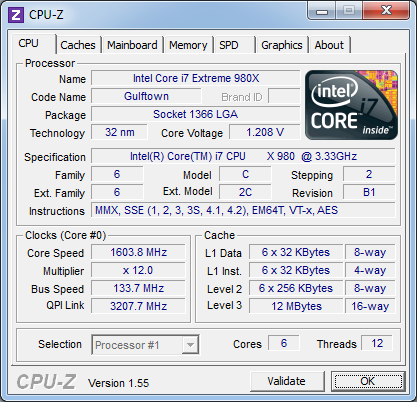
\includegraphics[scale=1]{imgs/cpu-z.png} 
\end{center}

%%%%%%%%%%%%%%%%%%%%%%%%%%%%%%%%%%%%%%%%%%%%%%%%%%%%%%%%%%%%%%%%

\newpage
\section{Трассировка лучей}
Классический ray tracing~[\cite{sivakov}], или метод трассировки лучей, предложен Артуром Аппелем (Arthur Appel) еще аж в 1968 году и дополнен алгоритмом общей рекурсии, разработанным Whitted в 1980 году. Понадобилось почти 12 лет эволюции вычислительных систем, прежде чем этот алгоритм стал доступен для широкого применения в практических приложениях. Реализация высокопроизводительной версии трассировки лучей уже предпринимаются различными компаниями. О сложности задачи трассировки лучей можно прочитать в соответствующих источниках~[\cite{biovulf}].

\subsection{Алгоритмы трассировки лучей}
Суть метода заключается в отслеживании траекторий лучей и расчета взаимодействий с лежащими на траекториях объектами, от момента испускания лучей источником света до момента попадания в камеру. Под взаимодействием луча с объектами понимаются процессы диффузного (в смысле модели локальной освещенности), многократного зеркального отражения от их поверхности и прохождение лучей сквозь прозрачные объекты. Таким образом, ray tracing – первый метод расчета глобального освещения, рассматривающий освещение, затенение (расчет тени), многократные отражения и преломления. Различают два основных вида метода трассировки лучей: \textbf{\textit{прямой}} -- \index{forward ray tracing}forward ray tracing, и \textbf{\textit{обратный}} -- \index{backward ray tracing}backward ray tracing.

\subsubsection{Прямой метод трассировки лучей}
В прямом методе траектории лучей строятся от источника ко всем точкам всех объектов сцены (первичные лучи). Затем проверяется ориентация каждой точки относительно источника, и, если она лежит на стороне объекта, обращенной в противоположную от источника сторону, точка из расчетов освещенности исключается. Для всех остальных точек вычисляется освещенность с помощью локальной модели освещения. Если объект не является отражающим или прозрачным, то есть поверхность объекта только диффузно рассеивает свет, траектория луча на этой точке обрывается (заканчивается). Если же поверхность объекта обладает свойством отражения (\index{reflection}reflection) и/или преломления (\index{refraction}refraction), из точки строятся новые лучи, направления которых совершенно точно определяются законами отражения и преломления.
\par
    Для построенных таким образом траекторий новых лучей может быть только три исхода. Луч либо выходит за пределы видимой из камеры области сцены, в этом случае все проделанные для него до этого момента расчеты освещенности отбрасываются, поскольку они не принимают участия в формировании изображения. Или луч попадает в камеру, тогда рассчитанная освещенность формирует цвет соответствующего пиксела изображения. Или луч встречает на своем пути новый
объект, тогда для новой точки пересечения повторяется расчет освещенности и построения лучей отражения и преломления в зависимости от свойств поверхности объекта (рекурсия). Построение новых траекторий и расчеты ведутся до тех пор, пока все лучи либо попадут в камеру, либо выйдут за пределы видимой области. Очевидно, что при прямой трассировке лучей мы вынуждены выполнять расчеты для лучей, которые не попадут в камеру, то есть, проделывать бесполезную работу. По некоторым оценочным данным доля таких "слепых"лучей довольно велика. Эта главная, хотя и далеко не единственная, причина того, что метод прямой трассировки лучей считается неэффективным и на практике не используется(в чистом виде).

\subsubsection{Обратный метод трассировки лучей}
Обратной метод трассировки лучей, или backward ray tracing. Этот метод расчетов основывается на построении лучей от наблюдателя через плоскость экрана вглубь сцены, а не от источника, то есть -- наоборот. Этот способ достаточно изящен, что позволяет решить массу проблем, возникающих при прямой трассировке, а сам метод отличается простотой и понятностью. Лучи теперь строятся иначе. А именно, по двум точкам: первая точка, общая для всех лучей – положение камеры (наблюдателя), вторая точка определяется положением пиксела на плоскости видового окна. Таким образом, направление каждого луча строго определено (две точки в пространстве определяют одну и только одну прямую – школьный курс геометрии), и количество первичных лучей также известно – это общее количество пикселей видового окна. Например, если видовое окно имеет 1920 пикселей по ширине и 1200 пикселей по высоте, количество лучей составит 1920 х 1200 = 2 304 000. Каждый луч
вдоль заданного направления продлевается от наблюдателя вглубь трехмерной сцены, и для каждой траектории выполняется проверка на пересечение со всеми объектами сцены и с отсекающими плоскостями. Если пересечений с объектами нет, а есть пересечение только с плоскостью отсечения, значит луч выходит за пределы видимой части сцены, и соответствующему пикселю видового окна присваивается цвет фона. Если луч пересекается с объектами сцены, то среди всех объектов выбирается тот, который ближе всего к наблюдателю. В точке пересечения с таким объектом строится три новых, так называемых вторичных луча. \par

\begin{center}
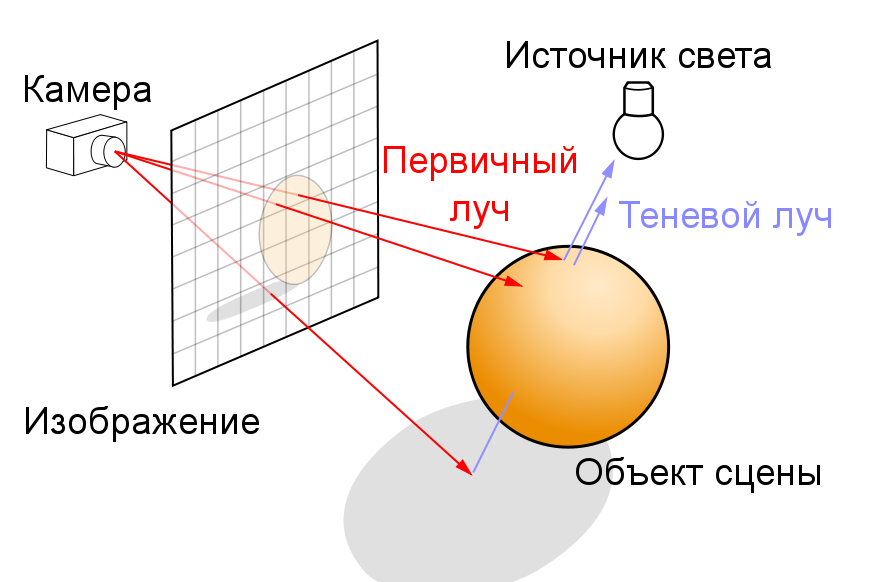
\includegraphics[scale=0.5]{imgs/Ray_trace_diagram_rus.png} 
\end{center}

Первый луч строится в направлении источника света. Если источников несколько, строится несколько таких лучей, по одному на каждый источник. Основное назначение этого луча – определить ориентацию точки (обращена точка к источнику или от него), наличие объектов, закрывающих точку от источника света, и расстояние до источника света. Если точка обращена в противоположную сторону от источника света или закрыта другим непрозрачным объектом, освещенность от такого источника не рассчитывается, точка находится в тени. В случае затеняющего прозрачного объекта интенсивность освещения уменьшается в соответствии со степенью прозрачности. Если точка закрыта от освещения всеми источниками сцены, ей присваивается фоновый (\index{ambient или фоновый цвет}ambient) цвет. В противном случае точка освещена, интенсивность и цвет освещения рассчитываются при помощи локальной модели освещенности, как сумма освещенностей от всех источников, для которых эта точка не закрыта другими объектами. Этот тип луча получил название \index{shadow ray или теневой луч} \textit{\textbf{shadow ray}} (иногда его еще называют \index{illumination ray}illumination ray) – теневой луч. Если поверхность объекта не является отражающей и непрозрачна, теневой луч – единственный тип лучей который строится, траектория первичного луча обрывается (заканчивается), и дальнейшие расчеты не выполняются. Рассчитанный цвет (освещенности или тени) присваивается тому пикселю видового окна, через который проходит соответствующий первичный луч.
   \par
   Второй луч строится, если поверхность объекта обладает отражающими свойствами, и называется \index{reflection ray или отраженный луч} reflection ray, или луч отражения. Направление отраженного луча определяется по закону:
$$
	\vec{R} = \vec{I} - 2 \cdot \vec{N} (\vec{N} , \vec{I})
$$
где $\vec{R}$ - отраженный луч, $\vec{I}$ - падающий пераичный луч, $\vec{N}$ - нормаль к поверхности в точке соударения.
Для отраженного луча проверяется возможность пересечения с другими объектами сцены. Если пересечений нет, то интенсивность и цвет отраженного луча равна интенсивности и цвету фона. Если пересечение есть, то в новой точке снова строится три типа лучей – теневые, отражения и преломления.
Третий луч строится, если поверхность объекта прозрачна, и носит название \index{transparency ray или преломленный луч}transparency ray, т. е. луч преломленный. Направление для преломленного луча определяется следующим образом:
$$
 \vec{T} = \frac{n_1}{n_2} \cdot \vec{I} - \left[ \cos \alpha + \frac{n_1}{n_2} \cdot \left(\vec{N},\vec{I} \ \right) \right] \cdot \vec{N}
$$
$$
\cos \alpha = \sqrt{1 - \left( \frac{n_1}{n_2} \right) ^2 \cdot \left(1-\left(\vec{N},\vec{I}\ \right)^2\right)}
$$
где $\vec{T}$ - переломленный луч, $n_1$ - коэффициент рефракции для первой среды ( в которой растространяется первичный луч ), $n_2$ - коэффициент рефракции для второй среды прозрачного объекта.

Так же, как и в предыдущем случае, проверяется пересечение вновь построенного луча с объектами, и, если они есть, в новой точке строятся три луча, если нет -- используется интенсивность и цвет фона.

Таким образом, для каждого первичного луча можно построить древовидную структуру. Если древовидная структура для данного луча построена, то расчет освещенности можно выполнить в следующем порядке. Для каждой ветви дерева спускаемся вдоль древовидной структуры к последнему пересечению вторичного луча и поверхности (будем дальше называть их узлами). Поскольку это последний узел в цепи, то  вкладов от преломлений и отражений нет, поэтому, освещенность узла вычисляется при помощи локальной модели освещения с учетом видимости источников света для данного узла. Затем, вычисленная освещенность передается вверх по ветви к следующему ближайшему узлу. Освещенность в этом узле будет вычисляться по формуле:

$$
 \vec{I}_{total} = \vec{I}_{local} + K_{reflection} \cdot \vec{I}_{reflection} + K_{refraction} \cdot \vec{I}_{refraction}
$$

где $\vec{I}_{total}$ - полная освещенность в точке, $\vec{I}_{local}$ - локальная освещенность в точке, вычисленная от источников освещения с помощью одной из локальной модели освещенности, $K_{reflection}$ - коэффициент, определяющий отражающие свойства поверхности, $\vec{I}_{reflection}$ - освещенность предыдущей точки, переданная вдоль ветки отражения,   $K_{refraction}$ - коэффициент, определяющий преломляющие свойства поверхности $\vec{I}_{refraction}$ - освещенность предыдущей точки, переданная вдоль ветки преломления

Естественным завершением трассировки лучей является выход всех испущенных вторичных лучей за пределы видимой области и их рассеяние на чисто диффузных объектах. Результат вычислений будет наиболее точным. Но, если сцена достаточно сложна, такой расчет будет очень медленным, а в некоторых случаях и невозможным по причине ограниченности аппаратных ресурсов. Легко увидеть, что вклад освещенности от каждого нового вторичного луча очень быстро уменьшается по той простой причине, что коэффициенты свойств отражения и преломления материалов меньше единицы. Поэтому часто трассировку лучей прекращают, когда вклад от следующего узла ветви становится меньше заданной величины. Это также достаточно точный метод расчетов, который может быть использован для получения качественных результатов при определенных условиях. Наконец, для получения оценочного расчета можно оборвать трассировку лучей после выполнения заданного количества итераций, это самый быстрый и наименее точный расчет.

\subsubsection{Достоинства и недостатки}

Основные достоинства рекурсивного метода обратной трассировки лучей – расчет теней, многократных отражений и преломлений, значительно повысивших степень реалистичности получаемых изображений.
Основные недостатки: неучет вторичного освещения от диффузно отраженного объектами света; низкая скорость и высокая вычислительная стоимость расчетов – в классическом рейтресинге необходимо проверять на пересечение каждый луч со всеми объектами сцены, в результате от 70 до 95 процентов всего времени расчетов тратится на вычисление пересечений; резкие границы цветовых переходов тени/подсветок/прозрачности; \index{aliasing}aliasing – "зазубренность" линий и т. д.; дискретность определяющих цвет пиксела первичных лучей – одного первичного луча недостаточно для корректного определения цвета пиксела, формирующего изображение.


\subsection{Модели освещения}

В соответствии с принятым в компьютерной графике подходом, расчет освещенности распадается на две основные задачи. Первая – определить способ расчета освещенности в произвольной точке трехмерного пространства, решается при помощи построения обобщенной математической модели освещенности (Illuminating model). Вторая задача – применение Illuminating model для компьютерных расчетов освещенности трехмерных объектов с конкретной геометрией и свойствами поверхности, решается при помощи так называемой модели затенения (Shading model).

Моделей освещенности к настоящему моменту разработано несколько. Самая первая,и самая простая – локальная модель освещенности. Эта модель не рассматривает процессы светового взаимодействия объектов сцены между собой, а только расчет освещенности самих объектов. Вторая, глобальная модель освещенности – Global Illuminations, рассматривает трехмерную сцену как единую систему и пытается описывать освещение с учетом взаимного влияния объектов. В рамках этой модели рассматриваются такие вопросы, как многократное отражение и преломление света (ray tracing), рассеянное освещение (radiosity), каустик(caustic) и фотонные карты (photon mapping) и другие. 

\subsubsection{Глобальные модели освещения}

Глобальное освещение (global illumination) — это название ряда алгоритмов, используемых в 3D-графике, которые предназначены для добавления более реалистичного освещения в трёхмерные сцены. Такие алгоритмы учитывают не только свет, который поступает непосредственно от источника света (прямое освещение, англ. direct illumination), но и такие случаи, в которых лучи света от одного и того же источника, отражаются на других поверхностях сцены (непрямая освещенность, англ. indirect illumination).

Теоретически отражение, преломление, тень — примеры глобального освещения, потому что, для их имитации необходимо учитывать влияние одного объекта на другие (в отличие от случая когда на объект падает прямой свет). На практике, однако, только моделирование диффузного отражения или каустики называется глобальным освещением.

Изображения полученные в результате применения алгоритмов глобального освещения часто кажутся более фотореалистичными, чем те, в процессе рендеринга которых применялись алгоритмы только прямого освещения, но для просчета глобального освещения требуется гораздо больше времени.

\subsubsection{Локальные модели освещения}

Существующие локальные модели освещения можно разделить на две категории. К первой категории относятся эмпирические модели. Они обычно эффективны в плане быстродействия и некоторые из них дают довольно реалистичную картинку. Они обычно не оперируют такими физическими величинами, как световая энергия, или световой поток. Однако эти модели находят довольно широкое применение в областях, где не требуется точная физическая информация об освещении (например, спецэффекты в фильмах, программы для художников и дизайнеров, для рекламных целей)

Ко второй категории относятся модели, базирующиеся на физических представлениях о теории света. Изображения, полученные с использованием этих моделей, очень хорошо соотносятся с экспериментальными данными. Поэтому эти модели находят применение там, где важна точная имитация поведения света (оформление интерьеров, архитектура)

\subsubsection{Модель Фонга}

Это эмпирическая модель. В самом общем случае, в свете требования фотореалистичности, эта модель учитывает и неявное ambient-освещение. Ambient-освещение, или его еще называют фоновым (background), – это окружающее объект освещение от удаленных источников, чье положение и характеристики не известны. Необходимость учета ambient-освещения, пусть и очень грубо, обусловлена тем, что его вклад может быть достаточно велик – до 50\% от общей освещенности. В Local Illumination считают, что фоновое освещение задает цвет (и его интенсивность) объекта в отсутствии явных источников света или в тени. Не несет никакой информации об объекте, кроме значения простого цвета, равномерно заливающего контур объекта.

Интенсивность такого освещения постоянна и равномерно распределена во всем пространстве, расчет его отражения поверхностью выполняется по формуле:

$$
 \vec{I}_{amb} = K_{a} \cdot \vec{I}_{a}
$$

где $\vec{I}_{amb}$  - интенсивность отраженного ambient освещения, $K_{a}$ - коэффициент, характеризующий отражающие свойства поверхности для  ambient-освещения, $\vec{I}_{a}$ - исходная интенсивность ambient-света, падающего на поверхность.

Часть света от прямых источников зеркально отражается поверхностью, а остальной свет диффузно рассеивается во всех направлениях. Кроме чисто зеркального отражения, которое имеют идеально отполированные поверхности, различают так называемое glossiness или распределенное зеркальное отражение – отражение в некотором створе углов, а не на один единственный угол. Такое рассеяние света обусловлено микрорельефом ("шероховатостью") поверхности, то есть поверхность реальных объектов не является идеально гладкой, а состоит из большого количества микровыступов и впадин, которые зеркально отражают падающий свет под разными углами. Результатом glossy-отражения является specular highlight – яркий световой блик, имеющий размер в зависимости от степени шероховатости поверхности. 

Интенсивность рассеянного света зависит от угла падающего на поверхность света по закону Ламберта (Lambert):

$$
 \vec{I}_{diff} = K_{diff} \cdot \vec{I}_{d} \cdot \cos(\alpha)
$$
 
где $\vec{I}_{d}$ - интенсивность падающего на поверхность света, $K_{diff}$ - коэффициент, характеризующий рассеивающие свойства поверхности, $\cos(\alpha)$ - угол между направлением на источник света и нормалью поверхности

Другими словами, поверхность будет освещена больше, если свет падает на нее перпендикулярно ($\alpha = 0$), и меньше, если свет падает под любым другим углом, поскольку в этом случае увеличивается освещаемая площадь. Диффузно рассеянный свет является главным источником визуальной информации о геометрии трехмерных объектов.

Как было уже сказано ранее, свет отражается зеркально в некотором створе углов, и для большинства реальных материалов мы всегда видим зеркальную подсветку в форме светового пятна, а не в форме яркой точки. Поэтому, для расчета интенсивности зеркально отраженного света используется формула, предложенная Фонгом:

$$
 \vec{I}_{spec} = K_{spec} \cdot \vec{I}_{s} \cdot \cos^n(\beta)
$$

где $\vec{I}_{spec}$ - интенсивность зеркально отраженного света,  $\vec{I}_{s}$ - интенсивность источника света,  $\vec{K}_{s}$ - коэффициент, характеризующий свойства зеркального отражения поверхности
$\beta$ - угол между направлением идеального отражения и направлением на наблюдателя, степень $n$ определяет размер пятна светового блика, чем больше $n$, тем меньше световой блик, и тем ближе отражающие свойства поверхности к свойствам идеального зеркала.

Формула Фонга – пример компьютерной фикции, поскольку она не имеет физического смысла. Ее используют просто потому, что она дает хорошие практические результаты. 

Таким образом, локальная модель освещенности предполагает расчет отраженной фоновой освещенности, диффузного и зеркального отражения от прямых источников: 

$$
 \vec{I}_{local} =  K_{amb} \cdot \vec{I}_{amb} +  K_{diff} \cdot \vec{I}_{diff} \cdot \left( \vec{L},\vec{N} \right) + K_{spec} \cdot \vec{I}_{spec} \cdot \left( \vec{R},\vec{V} \right)^n
$$



\subsection{Примитивы}
\subsubsection{\index{Плоскость}Плоскость}
Для определения пресечения луча с плоскостью, необходимо найти точку в пространстве, которая будет удовлетворять двум уравнениям: уравнению луча и уравнению плоскости.
\par
Уравнение луча:
\begin{equation}
\left\{
\begin{array}{ccccc}
x & = & x_0 & + & t \cdot x_d \\
y & = & y_0 & + & t \cdot y_d \\
z & = & z_0 & + & t \cdot z_d \\
\end{array}
\right.
\label{equation_ray}
\end{equation}
или
$$
\vec{R}(t) = \vec{O} + t \cdot \vec{D}
$$
где $O = \VECXYZ{0} $ - начало луча, а $D = \VECXYZ{d} $ - направление луча. 
\par
Уравнение плоскости задается следующим образом:
\begin{equation}
Ax + By + Cz + D = 0
\label{equation_plane}
\end{equation}
\par
Для того, что бы найти точку пересечения луча с плоскостью, необходимо подставить уравнение (\ref{equation_ray}) в (\ref{equation_plane}):
$$
A(x_0 + t \cdot x_d) + B(y_0 + t \cdot y_d) + C(z_0 + t \cdot z_d) + D = 0
$$
Раскроем скобки и приведем подобные
$$
t(Ax_d + By_d + Cz_d ) + Ax_0 + By_0 + Cz_0 + D = 0
$$
найдем неизвестную величину t
$$
 t = - \frac{Ax_0 + By_0 + Cz_0 + D}{Ax_d + By_d + Cz_d}
$$
из уравнения видно, что луч либо пересекает плоскость в какой то точке, либо нет. Это связано с тем, что если $Ax_d + By_d + Cz_d = 0$, то плоскость и луч параллельны друг другу. Т.к. $P = \VEC{A}{B}{C} $ - это нормаль к поверхности, то из геометрии известно, что если $( D , P ) = 0$, то вектора параллельны.
\par
   Для того, что бы найти величину $t$, необходимо рассчитать всего несколько скалярных произведений:
$$
t = - \frac{(O, P) + D}{(D, P)}
$$
при условии, что $(D, P) \neq 0$

\subsubsection{\index{Сфера}Сфера}
Для сферы необходимо проделать те же выкладки.
Уравнение луча:
\begin{equation}
\left\{
\begin{array}{ccccc}
x & = & x_0 & + & t \cdot x_d \\
y & = & y_0 & + & t \cdot y_d \\
z & = & z_0 & + & t \cdot z_d \\
\end{array}
\right.
\label{equation_ray}
\end{equation}
или
$$
\vec{R}(t) = \vec{O} + t \cdot \vec{D}
$$
Уравнение сферы записывается следующем образом:
\begin{equation}
(x-x_c)^2 + (y-y_c)^2 + (z-z_c)^2 = r^2
\label{equation_sphere}
\end{equation}
где $S = \VECXYZ{c}$ - центр сферы, а $r$ - радиус. Подставим уравнение (\ref{equation_ray}) в (\ref{equation_sphere}):
$$
\left( (x_0 + t \cdot x_d) - x_c \right)^2 + 
\left( (y_0 + t \cdot y_d) - y_c \right)^2 + 
\left( (z_0 + t \cdot z_d) - z_c \right)^2 = r^2
$$
приведем это уравнение в виду
\begin{equation}
A \cdot t^2 + B \cdot t + C = 0
\label{equation_square}
\end{equation}
после раскрытия скобок и приведения подобных, получаем:
\par
$$
A = x^2_d + y^2_d + z^2_d
$$ 
\par
$$
B = 2x_d(x_0 - x_c) + 2y_d(y_0 - y_c)  + 2z_d(z_0 - z_c) 
$$ 
\par
$$
C = (x_0 - x_c)^2 + (y_0 - y_c)^2 + (z_0 - z_c)^2 
$$
Если уравнение (\ref{equation_square}) не имеет вещественных решений, то луч не пересекает сферу. Если имеется два решения, то наименьший положительный корень этого уравнения определит на луче ближайшую точку пересечения луча со сферой.
\par
Рассмотрим подробнее как вычисляются коэффициенты $A$, $B$, $C$:
\par
$$
A = x^2_d + y^2_d + z^2_d = (D, D)
$$ 
\par
$$
B = 2x_d(x_0 - x_c) + 2y_d(y_0 - y_c)  + 2z_d(z_0 - z_c)  = 2 \cdot (D, D - S)
$$ 
\par
$$
C = (x_0 - x_c)^2 + (y_0 - y_c)^2 + (z_0 - z_c)^2 = (O - S, O - S )
$$
Далее решаем обыкновенное квадратное уравнение и находим корни и получаем значение $t$
$$
t_{1,2} = \frac{-B \pm \sqrt{B^2 - 4 \cdot A \cdot C}}{2 \cdot A}
$$

$$
t_{1} = \frac{ - 2 \cdot (\vec{D}, \vec{D} - \vec{S}) + \sqrt{(2 \cdot (\vec{D}, \vec{D} - \vec{S}))^2 - 4 \cdot (\vec{D}, \vec{D}) \cdot (\vec{O} - \vec{S}, \vec{O} - \vec{S} )}}{2 \cdot (\vec{D}, \vec{D})}
$$

$$
t_{2} = \frac{ - 2 \cdot (\vec{D}, \vec{D} - \vec{S}) - \sqrt{(2 \cdot (\vec{D}, \vec{D} - \vec{S}))^2 - 4 \cdot (\vec{D}, \vec{D}) \cdot (\vec{O} - \vec{S}, \vec{O} - \vec{S} )}}{2 \cdot (\vec{D}, \vec{D})}
$$

\subsubsection{\index{Треугольник}Треугольник}
Алгоритм пересечения луча и треугольника основан на барицентрических координатах.
\par
Барицентрические координаты -- координаты точки $n$-мерного аффинного пространства $A^n$, отнесенные к некоторой фиксированной системе из $(n + 1)$-ой точки $p_0, p_1, \dots, p_n$ , не лежащих в $(n -1)$-мерном подпространстве. Пусть $z$ есть произвольная точка в $A^n$. Каждая точка $x \in A^n$ может быть единственным образом представлена в виде суммы
$$
	x = z + \alpha_1 \cdot z\vec{p_1} + \alpha_2 \cdot z\vec{p_2} + \cdots + \alpha_n \cdot z\vec{p_n} 
$$
где $\alpha_1, \alpha_2, \dots,  \alpha_n $ вещественные числа, удовлетворяющие условию
$$
\alpha_1 + \alpha_2 + \cdots + \alpha_n  = 1
$$
Числа $\alpha_1, \alpha_2, \dots,  \alpha_n $ называются барицентрическими координатами точки $x$. Легко видеть, что барицентрические координаты не зависят от выбора $z$.

Точка $T(u,v)$, принадлежащая треугольнику, может быть записана в виде:
\begin{equation}
\label{triangle_bar}
T(u,v) = (1-u-v)V_0 + uV_1 + vV_2
\end{equation}

\noindent где $(u,v)$ -- это бариецентрические координаты такие, что $u \geq 0$, $v \geq 0$ и $u + v \leq 1$

Вычисление пересечения между лучем(\ref{equation_ray}) и треугольником(\ref{triangle_bar}), это решение следующего уравнения:

$$
O + tD = (1-u-v)V_0 + uV_1 + vV_2
$$

\noindent после нескольких очевидных преобразований:

$$
O + tD = V_0 - uV_0 - vV_0 + uV_1 + vV_2
$$
$$
O - V_0 = - tD + uV_1 - uV_0 + vV_2 - vV_0
$$

$$
- tD + u(V_1 - V_0) + v(V_2 - V_0) = O - V_0
$$

\noindent получаем:

\begin{equation}
\label{ray_cross_tr}
\left[ -D, V_1 - V_0 , V_2 - V_0\right] 
\left[  
\begin{array}{c} t \\ u \\ v \\ \end{array}
\right] = O - V_0
\end{equation}

Что бы решить задачу, необходимо найти вектор $\VEC{t}{u}{v}$. Обозначив $E_1 = V_1 - V_0$, $E_2 = V_2 - V_0$ и $T = O - V_0$ решим уравнение (\ref{ray_cross_tr}), используя метод Крамера:

\begin{equation}
\label{ray_cross_tr_solv}
\left[  
\begin{array}{c} t \\ u \\ v \\ \end{array}
\right] = 
\frac{1}{| -D , E_1, E_2|} 
\left[  
	\begin{array}{lcccl}
	|& T , & E_1, &E_2 & | \\
	|&-D , & T  , &E_2 & | \\
	|&-D , & E_1, &T   & | \\
	\end{array}
\right] 
\end{equation}

\noindent Из курса линейной алгебры известно, что: $|A, B, C| = - (A \times C) \cdot B = - (C \times B) \cdot A$. Принимая во внимания этот факт, перепишем уравление (\ref{ray_cross_tr_solv}).

\begin{equation}
\label{ray_cross_tr_solv2}
\left[  
\begin{array}{c} t \\ u \\ v \\ \end{array}
\right] = 
\frac{1}{(D \times E_2)\cdot E_1} 
\left[  
	\begin{array}{c}
	(T \times E_1) \cdot E_2 \\
	(D \times E_2) \cdot T \\
	(T \times E_1) \cdot D \\
	\end{array}
\right] = 
\frac{1}{P \cdot E_1} 
\left[  
	\begin{array}{c}
	Q \cdot E_2 \\
	P \cdot T \\	
	Q \cdot D \\	
	\end{array}
\right]
\end{equation}
где $P = (D \times E_2)$ и $Q = T \times E_1$


%%%%%%%%%%%%%%%%%%%%%%%%%%%%%%%%%%%%%%%%%%%%%%%%%%%%%%%%%%%%%%%%%%%%%%%%%%%%%%%%%%%%%%%%%%%

\newpage
\section{Оптимизация}
Оптимизация -- как способ программирования по уровням архитектуры сверху вниз.

\subsection{Шаблоны C++}

\subsubsection{Понятие шаблона}

Шаблоны(Templates) были введены в язык C++ как средство, позволяющие параметризовать типы данных. Это связано с тем, что для классов или функций приходилось реализовывать одни и те же алгоритмы, но для разных типов данных. Получали дублирование кода, и тем самым росло число ошибок. 
Пример. Реализовать функцию, которая возвращает максимальное значение из 2 чисел.

\cppsource{src/deftemplate.tex}{Несколько реализация функции {\bf max}}

\noindent
и так далее. Приходится писать один и тот же код несколько раз. Во второй функции можно было допустить ошибку (например указать неправильный знак сравнения), которую потом очень трудно найти. Или наоборот, после обнаружения ошибки, придется править код во всех реализациях функции max (возможна ситуация, когда в нескольких местах ошибка была исправлена, а в остальных пропущена или забыта). С этими проблемами помогли справится шаблоны, которые параметризовали типы данных следующим образом:

\cppsource{src/definetemplate.tex}{Шаблонное определение функции {\bf max}}

%\noindent
Т. о. работу которую выполнял программист теперь выполняет компилятор. При вызове функции, в качестве параметров которых нужно сравнить два int, компилятор сам из шаблона выведет функцию max(int,int).
\subsubsection{Вычисление на шаблонах}
Сегодня шаблоны используют различным образом, не так как ожидали изобретатели
шаблонов С++. Сегодня программирование на шаблонах включают различные техники, такие как: обобщенное программирование, вычисление во время компиляции, шаблонные выражения(expression templates), мета-программирование, и др.

\noindent Рассмотрим пример вычисления факториала. \\
\noindent Факториал числа N это: $N! = N \cdot (N-1) \cdot \dots \cdot 1$

Рекурсивная реализация факториала, без использование шаблонов, приведена в следующем листинге:

\cppsource{src/rekfactorial.tex}{Рекурсивная реализация факториала}

Эту функцию следует использовать следующим образом:
\begin{verbatim}
cout << factorial(7) << endl;
\end{verbatim}
Вызывать рекурсивно функцию - это очень большие накладные расходы. Несмотря на то, что мы указало компилятору встроить функцию (inline), компилятор проигнорирует это, так как он не может сделать постановку в рекурсию. Можно добиться большего успеха, если реализовывать это, как класс с шаблоном.

\cppsource{src/templatefactorial.tex}{Реализация факториала на шаблонах}

Можно заметить, что у данного шаблона нет ни данных, ни функциональных участков, это только определение перечислимого типа. Для того чтобы можно было определить шаблон для n, нужно для начала определить шаблон для n-1, т. е. для n-2, n-3 и т. д. В итоге получаем рекурсию. Следует заметить, что в качестве параметра шаблона используется обычный тип int. По стандарту, в качестве параметров шаблона могут быть использованы только перечислимые типы. В нашем случае есть параметр шаблона типа int, это означает, что в этот шаблон будет подставлено постоянное число типа int. Что бы воспользоваться данным классом необходимо написать следующие:
\begin{verbatim}
cout << factorial<7>::ret << endl;
\end{verbatim}
Компилятор рекурсивно определяет значение факториала<7>, затем <6> и так далее. Так как это рекурсия, то что бы не зациклится необходимо вовремя остановится. Любая рекурсия нуждается в остановки, и это не исключение. Это можно сделать с помощью специализации шаблона(т.е. определение для частного случая).

\cppsource{src/specfactorial.tex}{Специализация шаблона вычисления факториала}

Когда компилятор начнет определять специализацию для <0>, то он подставит имеено эту реализацию и рекурсия завершится. В результате, получится следующая структура:

\cppsource{src/finfactorial.tex}{Развернутая структура вычисления факториала}

Как видно из примера, от структуры уже ничего ни осталось и при уровне оптимизации начиная с O1, компилятор подсчитает выражение и вместо:
\begin{verbatim}
cout << factorial<7>::ret << endl;
\end{verbatim}
Подставит, подсчитанное выражение:
\begin{verbatim}
cout << 5040 << endl;
\end{verbatim}
Проверить это можно дизассемблировав данный пример и увидеть в коде число 5040.

\subsection{SIMD инструкции}
Применение SIMD инструкций в классе vec4.

\subsection{Ускоряющие структуры}
BVH. Алгоритмы построения и поиска.

%%%%%%%%%%%%%%%%%%%%%%%%%%%%%%%%%%%%%%%%%%%%%%%%%%%%%%%%%%%%%%%%%%%%%%%%%%%%%%%%%%%%%%%%%%%

\newpage
\section{Постановка и результаты экспериментов}

Эксперименты проводилимь на 6 ядерном компьютере с процессором Intel Core i7 980x с частотой 3.33GHz, оперативной памятью 12 Гб, ОС - Calculate Linux 11.0 x64. 

Для сборки приложения с библиотекой tbb, необходимо, что бы компилятор поддерживал лямбда выражения из нового стандарта c++0x. На данный момент, этот стандарт поддерживает компилятор GCC 4.5.2

\subsection{Timer}
Для того, чтобы точно оценивать время работы каждого из алгоритмов, очень важно иметь такой инструмент как таймер, способный оценить время работы алгоритма. 
Проблема в том, что стандарные методы операционных систем не работают с нужной точностью. Когда идет речь о том, чтобы оценить время, который должен исполнятся очень много миллионов раз в секунду, важен каждый такт процессора и точность в миллисекунду и уж тем более в секундах просто неприемлема.

Для очень точной оценки времени работы алгоритмов, был специально написан высокоточный таймер на языке c++, с использованием ассемблера (AT\&T - синтаксиса).
Таймер выдает время в тактах процессора и включает в себя разные режимы подсчета времени.

\subsubsection{Алгоритм работы высокоточного таймера}

\cppsource{src/timer.tex}{Метод Start() и Stop() класса Timer}


\subsubsection{Эксперименты с высокоточным таймером}

\subsection{Вектора и Expression templates}

\subsection{Тестовая сцена}

\subsection{Эффективность расспаралеливания}

\subsection{TBB vs OpenMP}

\subsection{Влияние SIMD инструкций на скорость работы}

\subsection{Компилирование высокоуровнего кода в ассемблер}

Ассемблерные вставки, которые показывают что вычисление отражающего луча это одно SSE.

%%%%%%%%%%%%%%%%%%%%%%%%%%%%%%%%%%%%%%%%%%%%%%%%%%%%%%%%%%%%%%%%%%%%%%%%%%%%%%%%%%%%%%%%%%%

\newpage
\section*{Заключение}
\addcontentsline{toc}{section}{Заключение} 
Задача трассировки лучей является по настоящему трудным испытанием для центрального процессора. Несмотря на то, что процессор обладает хорошей производительностью на ядро, общей производительности ему не хватает. Несмотря на столь малые мощности, удалось реализовать достаточно быстрый алгоритм на центральном процессоре. Для большей производительности была разработана эффективная параллельная версия программы с использованием библиотеки TBB и
стандарта параллельного OpenMP. Благодаря использованию языка с++ и технику шаблонных выражений, удалось еще повысить производительность программы. Программа продемонстрировала хорошую производительность: используя всего лишь один процессор можно получать изображения в реальном времени.

%%%%%%%%%%%%%%%%%%%%%%%%%%%%%%%%%%%%%%%%%%%%%%%%%%%%%%%%%%%%%%%%%%%%%%%%%%%%%%%%%%%%%%%%%%%

\newpage
\begin{thebibliography}{99}
	\bibitem{morozov_kazan} Морозов А. С. Трассировка лучей в реальном времени на многоядерном процессоре. Высокопроизводительные параллельные вычисления на кластерных системах (HPC-2008). Материалы Восьмой Международной конференции-семинара. Казань, ноябрь 17-19, 2008. Труды конференции — Казань: Изд. КГТУ, 2008. - С. 241.
	\bibitem{morozov_microsoft} Морозов А. С. Высокопроизводительная реализация трассировки лучей с использованием Microsoft MPI. Технологии Microsoft в теории и практике программирования. Материалы конференции /Под ред. Проф. В.П. Гергеля. - Нижний Новгород: Изд-во Нижегородского госуниверситета, 2009. - 527 с.
	\bibitem{morozov_pavt} Морозов А. С. Сравнительный анализ алгоритма трассировки лучей на системах с общей и разделяемой памятью. Параллельные вычислительные технологии (ПаВТ’2009): Труды международной научной конференции (Нижний Новгород, 30 марта - 3 апреля 2009 г.). - Челябинск: Изд. ЮурГУ, 2009. - 839 с
	\bibitem{latex} Львовский С.М. Набор и верстка в системе \LaTeX. – 4-е изд., стереотипн. – М.: МЦНМО, 2006
	\bibitem{alloftex} Кнут, Дональд, Э. Все про \TeX. : Пер. с англ. --- М. : Издательский дом ''Вильямс'', 2003. --- 560 с. : ил. --- Парал. Тит. англ.
	\bibitem{inteloptimize} Гербер Р., Бик А., Смит К., Тиан К. Оптимизация ПО. Сборник рецептов. --- СПб.: Питер, 2010. --- 352 с.: ил. --- (Серия ''Библиотека программиста'').
	\bibitem{templatecpp} Вандевурд, Дэвид, Джосаттис, Николаи М. Шаблоны C++: справочник разработчика. : Пер. с англ. --- М. : Издательский дом ''Вильямс'', 2008. --- 544 с. : ил. --- парал. тит. англ.
	\bibitem{straustrupcpp} Б. Страуструп Язык программирования C++. Специальное издание / Пер. с англ. --- М.: ООО ''Бином-Пресс'', 2006. --- 1104 с.: ил.
	\bibitem{sivakov} Сиваков И. Как компьютер рассчитывает изображения. Технология программного рендеринга, 11.03.2004. \\ (\href{http://www.fcenter.ru/online.shtml?articles/hardware/videos/8749}{http://www.fcenter.ru/online.shtml?articles/hardware/videos/8749})
	\bibitem{biovulf} Дмитрий Мороз. "Беовульф": Создание фильма, 11.12.2007.\\ (\href{http://www.3dnews.ru/editorial/beowulf}{http://www.3dnews.ru/editorial/beowulf})
	\bibitem{intelintrinsic} Intel® C++ Intrinsics Reference \\ (\href{http://www.intel.com/products/processor/manuals/}{http://www.intel.com/products/processor/manuals/})
	\bibitem{intelmanual} Intel 64 and IA-32.Architectures Software Developer's Manual \\ (\href{http://www.intel.com/products/processor/manuals/}{http://www.intel.com/products/processor/manuals/})
	\bibitem{tbbtutor} Intel® Threading Building Blocks. Tutorial \\ (\href{http://www.threadingbuildingblocks.org/}{http://www.threadingbuildingblocks.org/})
	\bibitem{tbbmanual} Intel® Threading Building Blocks. Reference Manual \\ (\href{http://www.threadingbuildingblocks.org/}{http://www.threadingbuildingblocks.org/})
	\bibitem{cppexpressiontemplate} C++ Expression Templates An Introduction to the Principles of Expression Templates, 2003 \\ (\href{http://www.angelikalanger.com/Articles/Cuj/ExpressionTemplates/ExpressionTemplates.htm}{http://www.angelikalanger.com/.../ExpressionTemplates.htm})
	\bibitem{intelcore980x} Шесть ядер для десктопа: Intel Core i7-980X Extreme Edition, 07.04.2010 \\ (\href{http://www.fcenter.ru/online.shtml?articles/hardware/processors/28480}{http://www.fcenter.ru/online.shtml?articles/hardware/processors/28480})
	\bibitem{rdtscp} How to Benchmark Code Execution Times on Intel IA-32 and IA-64 Instruction Set Architectures. September 2010
\end{thebibliography}

\newpage
\documentclass[12pt, a4paper]{article}
\usepackage[utf8]{inputenc}
\usepackage[russian]{babel} 
\usepackage[T2A]{fontenc}
\usepackage[pdftex]{graphicx}
\usepackage{amstext}
\usepackage{textcomp}
\usepackage{multicol}
\usepackage{hyperref}
\usepackage{setspace}
\usepackage[usenames,dvipsnames]{color} % для source-highlight
\usepackage{indentfirst}

% меняем размеры страницы
\usepackage{geometry}
\geometry{left=2.5cm}
\geometry{right=2.0cm}
\geometry{top=1.5cm}
\geometry{bottom=2.5cm}

% шрифты
%\defaultfontfeatures{Scale=MatchLowercase}
%\setmainfont[SmallCapsFont={* Caps}]{Liberation Serif}
%\usepackage{xltxtra}
%\setmainfont[Mapping=tex-text]{Linux Libertine O}
%\setmonofont[SmallCapsFont={Courier New}]{Courier New}
%\fontsize{10}{10}


%\usepackage{courier}
%\setmainfont[Mapping=tex-text]{Courier}


% изменение межстрочного интервала
\def\heightline{1.2}
\linespread{\heightline} % 1.3 - это полуторный

%%%%%%%%%%%%%%%%%%%%%%%%%%%%%%%%%%%%%%%%%%%%%%%%
%%% добавляем точки в Оглавление

\renewcommand{\thesection}{\arabic{section}.} 
\renewcommand{\thesubsection}{\arabic{section}.\arabic{subsection}.} 
\renewcommand{\thesubsubsection}{\arabic{section}.\arabic{subsection}.\arabic{subsubsection}.} 

%%%%%%%%%%%%%%%%%%%%%%%%%%%%%%%%%%%%%%%%%%%%%%%%

% определим новые команды
\def\VEC#1#2#3{\left( \begin{array}{c} #1 \\ #2 \\ #3 \end{array} \right) }
\def\VECXYZ#1{\left( \begin{array}{c} x_#1 \\ y_#1 \\ z_#1 \end{array} \right) }

\newcommand{\HRule}{\noindent\rule{\linewidth}{0.45mm}}

\newcounter{sourcecode}
\setcounter{sourcecode}{1}
\newcommand*{\cppsource}[2]{\par{\HRule \small \tt \bf \noindent \ Листинг \arabic{sourcecode}. {\rm \small #2} \vspace{0.25cm}}%
\addtocounter{sourcecode}{1} \input{#1} \HRule}

\makeindex

\begin{document}

\begin{titlepage}
\begin{center}
{\large Федеральное агентство по образованию Российской Федерации\\
\vspace{0.25em}
Государственное образовательное учреждение\\высшего профессионального образования\\Нижегородский государственный университет им. Н.И. Лобачевского\\
\vspace{0.25em}
Факультет вычислительной математики и кибернетики\\
\vspace{0.25em}
Кафедра математического обеспечения ЭВМ\\
\vspace{3em}
Дипломная работа\\
}
\vspace{1em}
{\bf \huge
	\textsf{ Трассировка лучей в реальном времени на x64~архитектуре \\ } 
}
\end{center}
\vspace{0.5cm}
\begin{multicols}{2}
\large 
\noindent 
Работа допущена к защите \\
Заведующий кафедрой МО ЭВМ \\
д.ф.--м.н., проф. \\

\vspace*{1em}
{ \noindent
\hspace*{1.5cm}\hbox to 0cm{\raisebox{-1em}{\small Подпись}}\hspace{-1.5cm}{\hrulefill\ Стронгин Р. Г. }
}

\vspace*{1.0em}
{ \noindent
\hbox to 0cm{\raisebox{0.25em}{<<\ \ \ \ \ \  >>}}{\hrulefill\ 2011 г. }
}
\vbox to 5 cm{\ }
Исполнитель: \\
студент 2 курса магистратуры \\
факультета ВМК группы 86М1 \\

\vspace*{1em}
{ \noindent
\hspace*{1.5cm}\hbox to 0cm{\raisebox{-1em}{\small Подпись}}\hspace{-1.5cm}{\hrulefill\ Морозов А. С. }
}

\vspace*{1.0em}
{ \noindent
\hbox to 0cm{\raisebox{0.25em}{<<\ \ \ \ \ \  >>}}{\hrulefill\ 2011 г. }
}
\\
Научный руководитель: д. т. н., \\
профессор кафедры МО ЭВМ \\

\vspace*{1em}
{ \noindent
\hspace*{1.5cm}\hbox to 0cm{\raisebox{-1em}{\small Подпись}}\hspace{-1.5cm}{\hrulefill\ Турлапов В. Е. }
}

\vspace*{1.0em}
{ \noindent\newcommand{\z}{\textbf{Задача. }}
\hbox to 0cm{\raisebox{0.25em}{<<\ \ \ \ \ \  >>}}{\hrulefill\ 2011 г. }
}
\end{multicols}

\vfill 
\begin{center} 
{\rm \large Нижний Новгород \\ 2011 г.} 
\end {center} 
\end{titlepage} 

\tableofcontents

\newpage
\section*{Введение}
\addcontentsline{toc}{section}{Введение} 
В кино индустрии к современной компьютерной графике предъявляются серьезные требования физически корректного моделирования о освещения сцен, состоящая из множества примитивов с различными характеристиками взаимодействия со светом. Даже малейшие неточности, могут отбросить художественный или анимационный фильм в рубрику любительского кино, и при этом не принести ожидаемой прибыли. Особенные требования предъявляются именно к художественному фильму, т. к. используемые спец эффекты должны выглядеть настолько реалистично, что бы зритель не смог различить, где настоящий актер, а где рисованный двойник. Используя только физически правильные модели и алгоритмы можно обеспечить растущую потребность в более реалистичной трехмерной графике. \par
   С каждым новым фильмом, каждый из нас видит прогресс в компьютерной графике. Картинка становится все красочнее и правдоподобнее, но это все не дается просто так. Естественно, платить за это приходится высокой вычислительной трудоемкостью расчетов. Несомненно, что с каждым годом производительность вычислительной техники растет, но она сразу же «расходуются» на новые спецэффекты. Существует наблюдение, которое гласит, что время расчета одного кадра не изменяется. Среднее время расчета полного фильма 15 лет назад занимал около 10-12 месяцев, так и сегодня тратят столько же времени, хотя при этом, надо заметить, что производительность современных компьютеров в десятки, а то и в сотни раз превышает производительность компьютеров того времени. Со временем улучшается и требования к самому изображению. Если несколько лет
назад картинка с разрешением 1024х768 считалась излишеством в компьютерной графики, то уже сейчас это слишком мало и все считают де факто FullHD\footnote{ \index{FullHD}FullHD -- это разрешение экрана 1920х1080 пикселей} , хотя уже задумываются о еще лучшем качестве. В последний год компьютерная индустрия, дабы не потерять зрителя, начала использовать новые технологии — 3D, которая требует еще большей вычислительной мощности. \par
   Именно за последние несколько лет компьютеры стали по настоящему параллельными. Появились многоядерные процессоры. И именно по этому, что 15 лет назад было трудоемкой задачей рендеринга, то сейчас это можно получить почти в реальном времени при том же качестве результата.

\newpage 
\section{Постановка задачи}
Главной целью данной работы является разработка и исследование алгоритма трассировки лучей на архитектуре x64 с применением ускоряющей структуры. Для решения главной задачи, требуется решить ряд следующих подзадач:
\begin{itemize}
	\item Реализовать высокопроизводительный алгоритм трассировки лучей на центральном процессоре
	\item Реализация и исследование оптимизированной версии с использованием векторных расширений архитектуры x64
	\item Реализация и исследование специализированного класса векторов для алгоритма трассировки лучей основанного на технологии шаблонных выражений, с применением векторных оптимизаций  - \index{SIMD}SIMD\footnote{ Single Instruction, Multiple Data — Одна Инструкция, Много Данных } инструкции 
	\item Реализация параллельной версии алгоритма трассировки лучей с использованием OpenMP, TBB
	\item Сравнение параллельной версии алгоритма трассировки лучей с использованием библиотеки TBB и расширения языка OpenMP
	\item Реализация ускоряющей структуры
	\item Сравнение реализации алгоритма с использованием ускоряющей структуры и без нее
\end{itemize}
   В качестве основного языка программирования выбирается язык С++, а для отображения результатов — кроссплатформенная библиотека SDL. 
   
\newpage 
\section{Архитектура центрального процессора}
\subsection{Архитектура процессоров семейства x86}
Рассмотрим основные архитектурные особенности центрального процессора.
Одни из базовых понятий для производительности процессора:
\begin{itemize}
	\item Latency (Латентность команды) --- это число тактов, необходимое для завершения одной команды с момента готовности входных данных команды(выборки их из памяти) и начало ее выполнения
	\item Throughput (Пропускная способность команды) --- это число тактов ожидания, которое требуется процессору перед запуском на выполнение такой же команды
\end{itemize}   

\subsection{Архитектура процессоров семейства x64}
\subsubsection{Архитектура процессора Intel Core i7 980X}
\noindent{\bf\ttОбзор}\\
Intel Core i7 — семейство процессоров x86-64 Intel. Core i7 980X это процессор семейства Gulftown вышедшего в 2010 году. Основные характеристики представлены с помощью программы cpu-z:
\begin{center}
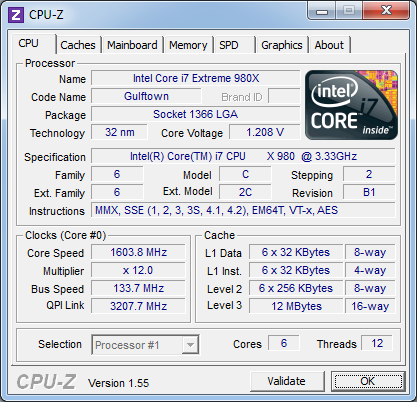
\includegraphics[scale=1]{imgs/cpu-z.png} 
\end{center}

%%%%%%%%%%%%%%%%%%%%%%%%%%%%%%%%%%%%%%%%%%%%%%%%%%%%%%%%%%%%%%%%

\newpage
\section{Трассировка лучей}
Классический ray tracing~[\cite{sivakov}], или метод трассировки лучей, предложен Артуром Аппелем (Arthur Appel) еще аж в 1968 году и дополнен алгоритмом общей рекурсии, разработанным Whitted в 1980 году. Понадобилось почти 12 лет эволюции вычислительных систем, прежде чем этот алгоритм стал доступен для широкого применения в практических приложениях. Реализация высокопроизводительной версии трассировки лучей уже предпринимаются различными компаниями. О сложности задачи трассировки лучей можно прочитать в соответствующих источниках~[\cite{biovulf}].

\subsection{Алгоритмы трассировки лучей}
Суть метода заключается в отслеживании траекторий лучей и расчета взаимодействий с лежащими на траекториях объектами, от момента испускания лучей источником света до момента попадания в камеру. Под взаимодействием луча с объектами понимаются процессы диффузного (в смысле модели локальной освещенности), многократного зеркального отражения от их поверхности и прохождение лучей сквозь прозрачные объекты. Таким образом, ray tracing – первый метод расчета глобального освещения, рассматривающий освещение, затенение (расчет тени), многократные отражения и преломления. Различают два основных вида метода трассировки лучей: \textbf{\textit{прямой}} -- \index{forward ray tracing}forward ray tracing, и \textbf{\textit{обратный}} -- \index{backward ray tracing}backward ray tracing.

\subsubsection{Прямой метод трассировки лучей}
В прямом методе траектории лучей строятся от источника ко всем точкам всех объектов сцены (первичные лучи). Затем проверяется ориентация каждой точки относительно источника, и, если она лежит на стороне объекта, обращенной в противоположную от источника сторону, точка из расчетов освещенности исключается. Для всех остальных точек вычисляется освещенность с помощью локальной модели освещения. Если объект не является отражающим или прозрачным, то есть поверхность объекта только диффузно рассеивает свет, траектория луча на этой точке обрывается (заканчивается). Если же поверхность объекта обладает свойством отражения (\index{reflection}reflection) и/или преломления (\index{refraction}refraction), из точки строятся новые лучи, направления которых совершенно точно определяются законами отражения и преломления.
\par
    Для построенных таким образом траекторий новых лучей может быть только три исхода. Луч либо выходит за пределы видимой из камеры области сцены, в этом случае все проделанные для него до этого момента расчеты освещенности отбрасываются, поскольку они не принимают участия в формировании изображения. Или луч попадает в камеру, тогда рассчитанная освещенность формирует цвет соответствующего пиксела изображения. Или луч встречает на своем пути новый
объект, тогда для новой точки пересечения повторяется расчет освещенности и построения лучей отражения и преломления в зависимости от свойств поверхности объекта (рекурсия). Построение новых траекторий и расчеты ведутся до тех пор, пока все лучи либо попадут в камеру, либо выйдут за пределы видимой области. Очевидно, что при прямой трассировке лучей мы вынуждены выполнять расчеты для лучей, которые не попадут в камеру, то есть, проделывать бесполезную работу. По некоторым оценочным данным доля таких "слепых"лучей довольно велика. Эта главная, хотя и далеко не единственная, причина того, что метод прямой трассировки лучей считается неэффективным и на практике не используется(в чистом виде).

\subsubsection{Обратный метод трассировки лучей}
Обратной метод трассировки лучей, или backward ray tracing. Этот метод расчетов основывается на построении лучей от наблюдателя через плоскость экрана вглубь сцены, а не от источника, то есть -- наоборот. Этот способ достаточно изящен, что позволяет решить массу проблем, возникающих при прямой трассировке, а сам метод отличается простотой и понятностью. Лучи теперь строятся иначе. А именно, по двум точкам: первая точка, общая для всех лучей – положение камеры (наблюдателя), вторая точка определяется положением пиксела на плоскости видового окна. Таким образом, направление каждого луча строго определено (две точки в пространстве определяют одну и только одну прямую – школьный курс геометрии), и количество первичных лучей также известно – это общее количество пикселей видового окна. Например, если видовое окно имеет 1920 пикселей по ширине и 1200 пикселей по высоте, количество лучей составит 1920 х 1200 = 2 304 000. Каждый луч
вдоль заданного направления продлевается от наблюдателя вглубь трехмерной сцены, и для каждой траектории выполняется проверка на пересечение со всеми объектами сцены и с отсекающими плоскостями. Если пересечений с объектами нет, а есть пересечение только с плоскостью отсечения, значит луч выходит за пределы видимой части сцены, и соответствующему пикселю видового окна присваивается цвет фона. Если луч пересекается с объектами сцены, то среди всех объектов выбирается тот, который ближе всего к наблюдателю. В точке пересечения с таким объектом строится три новых, так называемых вторичных луча. \par

\begin{center}
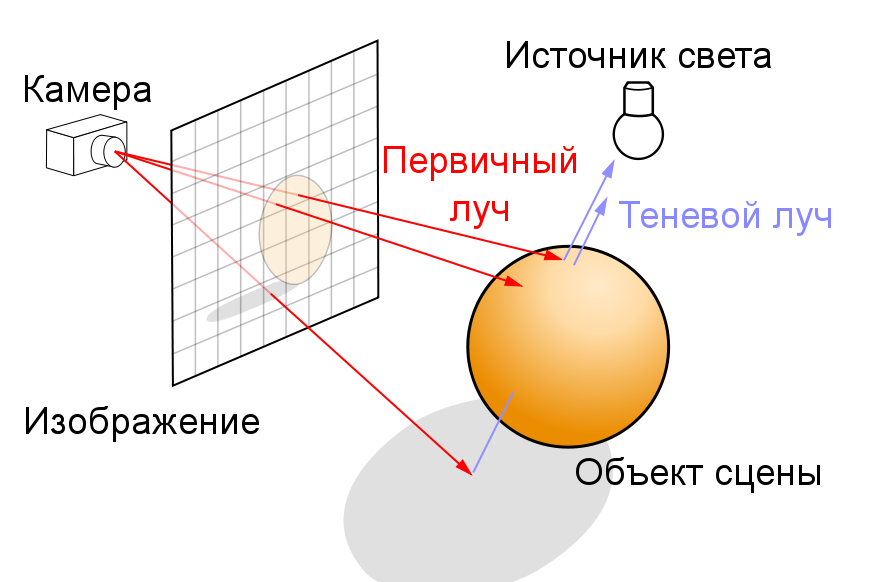
\includegraphics[scale=0.5]{imgs/Ray_trace_diagram_rus.png} 
\end{center}

Первый луч строится в направлении источника света. Если источников несколько, строится несколько таких лучей, по одному на каждый источник. Основное назначение этого луча – определить ориентацию точки (обращена точка к источнику или от него), наличие объектов, закрывающих точку от источника света, и расстояние до источника света. Если точка обращена в противоположную сторону от источника света или закрыта другим непрозрачным объектом, освещенность от такого источника не рассчитывается, точка находится в тени. В случае затеняющего прозрачного объекта интенсивность освещения уменьшается в соответствии со степенью прозрачности. Если точка закрыта от освещения всеми источниками сцены, ей присваивается фоновый (\index{ambient или фоновый цвет}ambient) цвет. В противном случае точка освещена, интенсивность и цвет освещения рассчитываются при помощи локальной модели освещенности, как сумма освещенностей от всех источников, для которых эта точка не закрыта другими объектами. Этот тип луча получил название \index{shadow ray или теневой луч} \textit{\textbf{shadow ray}} (иногда его еще называют \index{illumination ray}illumination ray) – теневой луч. Если поверхность объекта не является отражающей и непрозрачна, теневой луч – единственный тип лучей который строится, траектория первичного луча обрывается (заканчивается), и дальнейшие расчеты не выполняются. Рассчитанный цвет (освещенности или тени) присваивается тому пикселю видового окна, через который проходит соответствующий первичный луч.
   \par
   Второй луч строится, если поверхность объекта обладает отражающими свойствами, и называется \index{reflection ray или отраженный луч} reflection ray, или луч отражения. Направление отраженного луча определяется по закону:
$$
	\vec{R} = \vec{I} - 2 \cdot \vec{N} (\vec{N} , \vec{I})
$$
где $\vec{R}$ - отраженный луч, $\vec{I}$ - падающий пераичный луч, $\vec{N}$ - нормаль к поверхности в точке соударения.
Для отраженного луча проверяется возможность пересечения с другими объектами сцены. Если пересечений нет, то интенсивность и цвет отраженного луча равна интенсивности и цвету фона. Если пересечение есть, то в новой точке снова строится три типа лучей – теневые, отражения и преломления.
Третий луч строится, если поверхность объекта прозрачна, и носит название \index{transparency ray или преломленный луч}transparency ray, т. е. луч преломленный. Направление для преломленного луча определяется следующим образом:
$$
 \vec{T} = \frac{n_1}{n_2} \cdot \vec{I} - \left[ \cos \alpha + \frac{n_1}{n_2} \cdot \left(\vec{N},\vec{I} \ \right) \right] \cdot \vec{N}
$$
$$
\cos \alpha = \sqrt{1 - \left( \frac{n_1}{n_2} \right) ^2 \cdot \left(1-\left(\vec{N},\vec{I}\ \right)^2\right)}
$$
где $\vec{T}$ - переломленный луч, $n_1$ - коэффициент рефракции для первой среды ( в которой растространяется первичный луч ), $n_2$ - коэффициент рефракции для второй среды прозрачного объекта.

Так же, как и в предыдущем случае, проверяется пересечение вновь построенного луча с объектами, и, если они есть, в новой точке строятся три луча, если нет -- используется интенсивность и цвет фона.

Таким образом, для каждого первичного луча можно построить древовидную структуру. Если древовидная структура для данного луча построена, то расчет освещенности можно выполнить в следующем порядке. Для каждой ветви дерева спускаемся вдоль древовидной структуры к последнему пересечению вторичного луча и поверхности (будем дальше называть их узлами). Поскольку это последний узел в цепи, то  вкладов от преломлений и отражений нет, поэтому, освещенность узла вычисляется при помощи локальной модели освещения с учетом видимости источников света для данного узла. Затем, вычисленная освещенность передается вверх по ветви к следующему ближайшему узлу. Освещенность в этом узле будет вычисляться по формуле:

$$
 \vec{I}_{total} = \vec{I}_{local} + K_{reflection} \cdot \vec{I}_{reflection} + K_{refraction} \cdot \vec{I}_{refraction}
$$

где $\vec{I}_{total}$ - полная освещенность в точке, $\vec{I}_{local}$ - локальная освещенность в точке, вычисленная от источников освещения с помощью одной из локальной модели освещенности, $K_{reflection}$ - коэффициент, определяющий отражающие свойства поверхности, $\vec{I}_{reflection}$ - освещенность предыдущей точки, переданная вдоль ветки отражения,   $K_{refraction}$ - коэффициент, определяющий преломляющие свойства поверхности $\vec{I}_{refraction}$ - освещенность предыдущей точки, переданная вдоль ветки преломления

Естественным завершением трассировки лучей является выход всех испущенных вторичных лучей за пределы видимой области и их рассеяние на чисто диффузных объектах. Результат вычислений будет наиболее точным. Но, если сцена достаточно сложна, такой расчет будет очень медленным, а в некоторых случаях и невозможным по причине ограниченности аппаратных ресурсов. Легко увидеть, что вклад освещенности от каждого нового вторичного луча очень быстро уменьшается по той простой причине, что коэффициенты свойств отражения и преломления материалов меньше единицы. Поэтому часто трассировку лучей прекращают, когда вклад от следующего узла ветви становится меньше заданной величины. Это также достаточно точный метод расчетов, который может быть использован для получения качественных результатов при определенных условиях. Наконец, для получения оценочного расчета можно оборвать трассировку лучей после выполнения заданного количества итераций, это самый быстрый и наименее точный расчет.

\subsubsection{Достоинства и недостатки}

Основные достоинства рекурсивного метода обратной трассировки лучей – расчет теней, многократных отражений и преломлений, значительно повысивших степень реалистичности получаемых изображений.
Основные недостатки: неучет вторичного освещения от диффузно отраженного объектами света; низкая скорость и высокая вычислительная стоимость расчетов – в классическом рейтресинге необходимо проверять на пересечение каждый луч со всеми объектами сцены, в результате от 70 до 95 процентов всего времени расчетов тратится на вычисление пересечений; резкие границы цветовых переходов тени/подсветок/прозрачности; \index{aliasing}aliasing – "зазубренность" линий и т. д.; дискретность определяющих цвет пиксела первичных лучей – одного первичного луча недостаточно для корректного определения цвета пиксела, формирующего изображение.


\subsection{Модели освещения}

В соответствии с принятым в компьютерной графике подходом, расчет освещенности распадается на две основные задачи. Первая – определить способ расчета освещенности в произвольной точке трехмерного пространства, решается при помощи построения обобщенной математической модели освещенности (Illuminating model). Вторая задача – применение Illuminating model для компьютерных расчетов освещенности трехмерных объектов с конкретной геометрией и свойствами поверхности, решается при помощи так называемой модели затенения (Shading model).

Моделей освещенности к настоящему моменту разработано несколько. Самая первая,и самая простая – локальная модель освещенности. Эта модель не рассматривает процессы светового взаимодействия объектов сцены между собой, а только расчет освещенности самих объектов. Вторая, глобальная модель освещенности – Global Illuminations, рассматривает трехмерную сцену как единую систему и пытается описывать освещение с учетом взаимного влияния объектов. В рамках этой модели рассматриваются такие вопросы, как многократное отражение и преломление света (ray tracing), рассеянное освещение (radiosity), каустик(caustic) и фотонные карты (photon mapping) и другие. 

\subsubsection{Глобальные модели освещения}

Глобальное освещение (global illumination) — это название ряда алгоритмов, используемых в 3D-графике, которые предназначены для добавления более реалистичного освещения в трёхмерные сцены. Такие алгоритмы учитывают не только свет, который поступает непосредственно от источника света (прямое освещение, англ. direct illumination), но и такие случаи, в которых лучи света от одного и того же источника, отражаются на других поверхностях сцены (непрямая освещенность, англ. indirect illumination).

Теоретически отражение, преломление, тень — примеры глобального освещения, потому что, для их имитации необходимо учитывать влияние одного объекта на другие (в отличие от случая когда на объект падает прямой свет). На практике, однако, только моделирование диффузного отражения или каустики называется глобальным освещением.

Изображения полученные в результате применения алгоритмов глобального освещения часто кажутся более фотореалистичными, чем те, в процессе рендеринга которых применялись алгоритмы только прямого освещения, но для просчета глобального освещения требуется гораздо больше времени.

\subsubsection{Локальные модели освещения}

Существующие локальные модели освещения можно разделить на две категории. К первой категории относятся эмпирические модели. Они обычно эффективны в плане быстродействия и некоторые из них дают довольно реалистичную картинку. Они обычно не оперируют такими физическими величинами, как световая энергия, или световой поток. Однако эти модели находят довольно широкое применение в областях, где не требуется точная физическая информация об освещении (например, спецэффекты в фильмах, программы для художников и дизайнеров, для рекламных целей)

Ко второй категории относятся модели, базирующиеся на физических представлениях о теории света. Изображения, полученные с использованием этих моделей, очень хорошо соотносятся с экспериментальными данными. Поэтому эти модели находят применение там, где важна точная имитация поведения света (оформление интерьеров, архитектура)

\subsubsection{Модель Фонга}

Это эмпирическая модель. В самом общем случае, в свете требования фотореалистичности, эта модель учитывает и неявное ambient-освещение. Ambient-освещение, или его еще называют фоновым (background), – это окружающее объект освещение от удаленных источников, чье положение и характеристики не известны. Необходимость учета ambient-освещения, пусть и очень грубо, обусловлена тем, что его вклад может быть достаточно велик – до 50\% от общей освещенности. В Local Illumination считают, что фоновое освещение задает цвет (и его интенсивность) объекта в отсутствии явных источников света или в тени. Не несет никакой информации об объекте, кроме значения простого цвета, равномерно заливающего контур объекта.

Интенсивность такого освещения постоянна и равномерно распределена во всем пространстве, расчет его отражения поверхностью выполняется по формуле:

$$
 \vec{I}_{amb} = K_{a} \cdot \vec{I}_{a}
$$

где $\vec{I}_{amb}$  - интенсивность отраженного ambient освещения, $K_{a}$ - коэффициент, характеризующий отражающие свойства поверхности для  ambient-освещения, $\vec{I}_{a}$ - исходная интенсивность ambient-света, падающего на поверхность.

Часть света от прямых источников зеркально отражается поверхностью, а остальной свет диффузно рассеивается во всех направлениях. Кроме чисто зеркального отражения, которое имеют идеально отполированные поверхности, различают так называемое glossiness или распределенное зеркальное отражение – отражение в некотором створе углов, а не на один единственный угол. Такое рассеяние света обусловлено микрорельефом ("шероховатостью") поверхности, то есть поверхность реальных объектов не является идеально гладкой, а состоит из большого количества микровыступов и впадин, которые зеркально отражают падающий свет под разными углами. Результатом glossy-отражения является specular highlight – яркий световой блик, имеющий размер в зависимости от степени шероховатости поверхности. 

Интенсивность рассеянного света зависит от угла падающего на поверхность света по закону Ламберта (Lambert):

$$
 \vec{I}_{diff} = K_{diff} \cdot \vec{I}_{d} \cdot \cos(\alpha)
$$
 
где $\vec{I}_{d}$ - интенсивность падающего на поверхность света, $K_{diff}$ - коэффициент, характеризующий рассеивающие свойства поверхности, $\cos(\alpha)$ - угол между направлением на источник света и нормалью поверхности

Другими словами, поверхность будет освещена больше, если свет падает на нее перпендикулярно ($\alpha = 0$), и меньше, если свет падает под любым другим углом, поскольку в этом случае увеличивается освещаемая площадь. Диффузно рассеянный свет является главным источником визуальной информации о геометрии трехмерных объектов.

Как было уже сказано ранее, свет отражается зеркально в некотором створе углов, и для большинства реальных материалов мы всегда видим зеркальную подсветку в форме светового пятна, а не в форме яркой точки. Поэтому, для расчета интенсивности зеркально отраженного света используется формула, предложенная Фонгом:

$$
 \vec{I}_{spec} = K_{spec} \cdot \vec{I}_{s} \cdot \cos^n(\beta)
$$

где $\vec{I}_{spec}$ - интенсивность зеркально отраженного света,  $\vec{I}_{s}$ - интенсивность источника света,  $\vec{K}_{s}$ - коэффициент, характеризующий свойства зеркального отражения поверхности
$\beta$ - угол между направлением идеального отражения и направлением на наблюдателя, степень $n$ определяет размер пятна светового блика, чем больше $n$, тем меньше световой блик, и тем ближе отражающие свойства поверхности к свойствам идеального зеркала.

Формула Фонга – пример компьютерной фикции, поскольку она не имеет физического смысла. Ее используют просто потому, что она дает хорошие практические результаты. 

Таким образом, локальная модель освещенности предполагает расчет отраженной фоновой освещенности, диффузного и зеркального отражения от прямых источников: 

$$
 \vec{I}_{local} =  K_{amb} \cdot \vec{I}_{amb} +  K_{diff} \cdot \vec{I}_{diff} \cdot \left( \vec{L},\vec{N} \right) + K_{spec} \cdot \vec{I}_{spec} \cdot \left( \vec{R},\vec{V} \right)^n
$$



\subsection{Примитивы}
\subsubsection{\index{Плоскость}Плоскость}
Для определения пресечения луча с плоскостью, необходимо найти точку в пространстве, которая будет удовлетворять двум уравнениям: уравнению луча и уравнению плоскости.
\par
Уравнение луча:
\begin{equation}
\left\{
\begin{array}{ccccc}
x & = & x_0 & + & t \cdot x_d \\
y & = & y_0 & + & t \cdot y_d \\
z & = & z_0 & + & t \cdot z_d \\
\end{array}
\right.
\label{equation_ray}
\end{equation}
или
$$
\vec{R}(t) = \vec{O} + t \cdot \vec{D}
$$
где $O = \VECXYZ{0} $ - начало луча, а $D = \VECXYZ{d} $ - направление луча. 
\par
Уравнение плоскости задается следующим образом:
\begin{equation}
Ax + By + Cz + D = 0
\label{equation_plane}
\end{equation}
\par
Для того, что бы найти точку пересечения луча с плоскостью, необходимо подставить уравнение (\ref{equation_ray}) в (\ref{equation_plane}):
$$
A(x_0 + t \cdot x_d) + B(y_0 + t \cdot y_d) + C(z_0 + t \cdot z_d) + D = 0
$$
Раскроем скобки и приведем подобные
$$
t(Ax_d + By_d + Cz_d ) + Ax_0 + By_0 + Cz_0 + D = 0
$$
найдем неизвестную величину t
$$
 t = - \frac{Ax_0 + By_0 + Cz_0 + D}{Ax_d + By_d + Cz_d}
$$
из уравнения видно, что луч либо пересекает плоскость в какой то точке, либо нет. Это связано с тем, что если $Ax_d + By_d + Cz_d = 0$, то плоскость и луч параллельны друг другу. Т.к. $P = \VEC{A}{B}{C} $ - это нормаль к поверхности, то из геометрии известно, что если $( D , P ) = 0$, то вектора параллельны.
\par
   Для того, что бы найти величину $t$, необходимо рассчитать всего несколько скалярных произведений:
$$
t = - \frac{(O, P) + D}{(D, P)}
$$
при условии, что $(D, P) \neq 0$

\subsubsection{\index{Сфера}Сфера}
Для сферы необходимо проделать те же выкладки.
Уравнение луча:
\begin{equation}
\left\{
\begin{array}{ccccc}
x & = & x_0 & + & t \cdot x_d \\
y & = & y_0 & + & t \cdot y_d \\
z & = & z_0 & + & t \cdot z_d \\
\end{array}
\right.
\label{equation_ray}
\end{equation}
или
$$
\vec{R}(t) = \vec{O} + t \cdot \vec{D}
$$
Уравнение сферы записывается следующем образом:
\begin{equation}
(x-x_c)^2 + (y-y_c)^2 + (z-z_c)^2 = r^2
\label{equation_sphere}
\end{equation}
где $S = \VECXYZ{c}$ - центр сферы, а $r$ - радиус. Подставим уравнение (\ref{equation_ray}) в (\ref{equation_sphere}):
$$
\left( (x_0 + t \cdot x_d) - x_c \right)^2 + 
\left( (y_0 + t \cdot y_d) - y_c \right)^2 + 
\left( (z_0 + t \cdot z_d) - z_c \right)^2 = r^2
$$
приведем это уравнение в виду
\begin{equation}
A \cdot t^2 + B \cdot t + C = 0
\label{equation_square}
\end{equation}
после раскрытия скобок и приведения подобных, получаем:
\par
$$
A = x^2_d + y^2_d + z^2_d
$$ 
\par
$$
B = 2x_d(x_0 - x_c) + 2y_d(y_0 - y_c)  + 2z_d(z_0 - z_c) 
$$ 
\par
$$
C = (x_0 - x_c)^2 + (y_0 - y_c)^2 + (z_0 - z_c)^2 
$$
Если уравнение (\ref{equation_square}) не имеет вещественных решений, то луч не пересекает сферу. Если имеется два решения, то наименьший положительный корень этого уравнения определит на луче ближайшую точку пересечения луча со сферой.
\par
Рассмотрим подробнее как вычисляются коэффициенты $A$, $B$, $C$:
\par
$$
A = x^2_d + y^2_d + z^2_d = (D, D)
$$ 
\par
$$
B = 2x_d(x_0 - x_c) + 2y_d(y_0 - y_c)  + 2z_d(z_0 - z_c)  = 2 \cdot (D, D - S)
$$ 
\par
$$
C = (x_0 - x_c)^2 + (y_0 - y_c)^2 + (z_0 - z_c)^2 = (O - S, O - S )
$$
Далее решаем обыкновенное квадратное уравнение и находим корни и получаем значение $t$
$$
t_{1,2} = \frac{-B \pm \sqrt{B^2 - 4 \cdot A \cdot C}}{2 \cdot A}
$$

$$
t_{1} = \frac{ - 2 \cdot (\vec{D}, \vec{D} - \vec{S}) + \sqrt{(2 \cdot (\vec{D}, \vec{D} - \vec{S}))^2 - 4 \cdot (\vec{D}, \vec{D}) \cdot (\vec{O} - \vec{S}, \vec{O} - \vec{S} )}}{2 \cdot (\vec{D}, \vec{D})}
$$

$$
t_{2} = \frac{ - 2 \cdot (\vec{D}, \vec{D} - \vec{S}) - \sqrt{(2 \cdot (\vec{D}, \vec{D} - \vec{S}))^2 - 4 \cdot (\vec{D}, \vec{D}) \cdot (\vec{O} - \vec{S}, \vec{O} - \vec{S} )}}{2 \cdot (\vec{D}, \vec{D})}
$$

\subsubsection{\index{Треугольник}Треугольник}
Алгоритм пересечения луча и треугольника основан на барицентрических координатах.
\par
Барицентрические координаты -- координаты точки $n$-мерного аффинного пространства $A^n$, отнесенные к некоторой фиксированной системе из $(n + 1)$-ой точки $p_0, p_1, \dots, p_n$ , не лежащих в $(n -1)$-мерном подпространстве. Пусть $z$ есть произвольная точка в $A^n$. Каждая точка $x \in A^n$ может быть единственным образом представлена в виде суммы
$$
	x = z + \alpha_1 \cdot z\vec{p_1} + \alpha_2 \cdot z\vec{p_2} + \cdots + \alpha_n \cdot z\vec{p_n} 
$$
где $\alpha_1, \alpha_2, \dots,  \alpha_n $ вещественные числа, удовлетворяющие условию
$$
\alpha_1 + \alpha_2 + \cdots + \alpha_n  = 1
$$
Числа $\alpha_1, \alpha_2, \dots,  \alpha_n $ называются барицентрическими координатами точки $x$. Легко видеть, что барицентрические координаты не зависят от выбора $z$.

Точка $T(u,v)$, принадлежащая треугольнику, может быть записана в виде:
\begin{equation}
\label{triangle_bar}
T(u,v) = (1-u-v)V_0 + uV_1 + vV_2
\end{equation}

\noindent где $(u,v)$ -- это бариецентрические координаты такие, что $u \geq 0$, $v \geq 0$ и $u + v \leq 1$

Вычисление пересечения между лучем(\ref{equation_ray}) и треугольником(\ref{triangle_bar}), это решение следующего уравнения:

$$
O + tD = (1-u-v)V_0 + uV_1 + vV_2
$$

\noindent после нескольких очевидных преобразований:

$$
O + tD = V_0 - uV_0 - vV_0 + uV_1 + vV_2
$$
$$
O - V_0 = - tD + uV_1 - uV_0 + vV_2 - vV_0
$$

$$
- tD + u(V_1 - V_0) + v(V_2 - V_0) = O - V_0
$$

\noindent получаем:

\begin{equation}
\label{ray_cross_tr}
\left[ -D, V_1 - V_0 , V_2 - V_0\right] 
\left[  
\begin{array}{c} t \\ u \\ v \\ \end{array}
\right] = O - V_0
\end{equation}

Что бы решить задачу, необходимо найти вектор $\VEC{t}{u}{v}$. Обозначив $E_1 = V_1 - V_0$, $E_2 = V_2 - V_0$ и $T = O - V_0$ решим уравнение (\ref{ray_cross_tr}), используя метод Крамера:

\begin{equation}
\label{ray_cross_tr_solv}
\left[  
\begin{array}{c} t \\ u \\ v \\ \end{array}
\right] = 
\frac{1}{| -D , E_1, E_2|} 
\left[  
	\begin{array}{lcccl}
	|& T , & E_1, &E_2 & | \\
	|&-D , & T  , &E_2 & | \\
	|&-D , & E_1, &T   & | \\
	\end{array}
\right] 
\end{equation}

\noindent Из курса линейной алгебры известно, что: $|A, B, C| = - (A \times C) \cdot B = - (C \times B) \cdot A$. Принимая во внимания этот факт, перепишем уравление (\ref{ray_cross_tr_solv}).

\begin{equation}
\label{ray_cross_tr_solv2}
\left[  
\begin{array}{c} t \\ u \\ v \\ \end{array}
\right] = 
\frac{1}{(D \times E_2)\cdot E_1} 
\left[  
	\begin{array}{c}
	(T \times E_1) \cdot E_2 \\
	(D \times E_2) \cdot T \\
	(T \times E_1) \cdot D \\
	\end{array}
\right] = 
\frac{1}{P \cdot E_1} 
\left[  
	\begin{array}{c}
	Q \cdot E_2 \\
	P \cdot T \\	
	Q \cdot D \\	
	\end{array}
\right]
\end{equation}
где $P = (D \times E_2)$ и $Q = T \times E_1$


%%%%%%%%%%%%%%%%%%%%%%%%%%%%%%%%%%%%%%%%%%%%%%%%%%%%%%%%%%%%%%%%%%%%%%%%%%%%%%%%%%%%%%%%%%%

\newpage
\section{Оптимизация}
Оптимизация -- как способ программирования по уровням архитектуры сверху вниз.

\subsection{Шаблоны C++}

\subsubsection{Понятие шаблона}

Шаблоны(Templates) были введены в язык C++ как средство, позволяющие параметризовать типы данных. Это связано с тем, что для классов или функций приходилось реализовывать одни и те же алгоритмы, но для разных типов данных. Получали дублирование кода, и тем самым росло число ошибок. 
Пример. Реализовать функцию, которая возвращает максимальное значение из 2 чисел.

\cppsource{src/deftemplate.tex}{Несколько реализация функции {\bf max}}

\noindent
и так далее. Приходится писать один и тот же код несколько раз. Во второй функции можно было допустить ошибку (например указать неправильный знак сравнения), которую потом очень трудно найти. Или наоборот, после обнаружения ошибки, придется править код во всех реализациях функции max (возможна ситуация, когда в нескольких местах ошибка была исправлена, а в остальных пропущена или забыта). С этими проблемами помогли справится шаблоны, которые параметризовали типы данных следующим образом:

\cppsource{src/definetemplate.tex}{Шаблонное определение функции {\bf max}}

%\noindent
Т. о. работу которую выполнял программист теперь выполняет компилятор. При вызове функции, в качестве параметров которых нужно сравнить два int, компилятор сам из шаблона выведет функцию max(int,int).
\subsubsection{Вычисление на шаблонах}
Сегодня шаблоны используют различным образом, не так как ожидали изобретатели
шаблонов С++. Сегодня программирование на шаблонах включают различные техники, такие как: обобщенное программирование, вычисление во время компиляции, шаблонные выражения(expression templates), мета-программирование, и др.

\noindent Рассмотрим пример вычисления факториала. \\
\noindent Факториал числа N это: $N! = N \cdot (N-1) \cdot \dots \cdot 1$

Рекурсивная реализация факториала, без использование шаблонов, приведена в следующем листинге:

\cppsource{src/rekfactorial.tex}{Рекурсивная реализация факториала}

Эту функцию следует использовать следующим образом:
\begin{verbatim}
cout << factorial(7) << endl;
\end{verbatim}
Вызывать рекурсивно функцию - это очень большие накладные расходы. Несмотря на то, что мы указало компилятору встроить функцию (inline), компилятор проигнорирует это, так как он не может сделать постановку в рекурсию. Можно добиться большего успеха, если реализовывать это, как класс с шаблоном.

\cppsource{src/templatefactorial.tex}{Реализация факториала на шаблонах}

Можно заметить, что у данного шаблона нет ни данных, ни функциональных участков, это только определение перечислимого типа. Для того чтобы можно было определить шаблон для n, нужно для начала определить шаблон для n-1, т. е. для n-2, n-3 и т. д. В итоге получаем рекурсию. Следует заметить, что в качестве параметра шаблона используется обычный тип int. По стандарту, в качестве параметров шаблона могут быть использованы только перечислимые типы. В нашем случае есть параметр шаблона типа int, это означает, что в этот шаблон будет подставлено постоянное число типа int. Что бы воспользоваться данным классом необходимо написать следующие:
\begin{verbatim}
cout << factorial<7>::ret << endl;
\end{verbatim}
Компилятор рекурсивно определяет значение факториала<7>, затем <6> и так далее. Так как это рекурсия, то что бы не зациклится необходимо вовремя остановится. Любая рекурсия нуждается в остановки, и это не исключение. Это можно сделать с помощью специализации шаблона(т.е. определение для частного случая).

\cppsource{src/specfactorial.tex}{Специализация шаблона вычисления факториала}

Когда компилятор начнет определять специализацию для <0>, то он подставит имеено эту реализацию и рекурсия завершится. В результате, получится следующая структура:

\cppsource{src/finfactorial.tex}{Развернутая структура вычисления факториала}

Как видно из примера, от структуры уже ничего ни осталось и при уровне оптимизации начиная с O1, компилятор подсчитает выражение и вместо:
\begin{verbatim}
cout << factorial<7>::ret << endl;
\end{verbatim}
Подставит, подсчитанное выражение:
\begin{verbatim}
cout << 5040 << endl;
\end{verbatim}
Проверить это можно дизассемблировав данный пример и увидеть в коде число 5040.

\subsection{SIMD инструкции}
Применение SIMD инструкций в классе vec4.

\subsection{Ускоряющие структуры}
BVH. Алгоритмы построения и поиска.

%%%%%%%%%%%%%%%%%%%%%%%%%%%%%%%%%%%%%%%%%%%%%%%%%%%%%%%%%%%%%%%%%%%%%%%%%%%%%%%%%%%%%%%%%%%

\newpage
\section{Постановка и результаты экспериментов}

Эксперименты проводилимь на 6 ядерном компьютере с процессором Intel Core i7 980x с частотой 3.33GHz, оперативной памятью 12 Гб, ОС - Calculate Linux 11.0 x64. 

Для сборки приложения с библиотекой tbb, необходимо, что бы компилятор поддерживал лямбда выражения из нового стандарта c++0x. На данный момент, этот стандарт поддерживает компилятор GCC 4.5.2

\subsection{Timer}
Для того, чтобы точно оценивать время работы каждого из алгоритмов, очень важно иметь такой инструмент как таймер, способный оценить время работы алгоритма. 
Проблема в том, что стандарные методы операционных систем не работают с нужной точностью. Когда идет речь о том, чтобы оценить время, который должен исполнятся очень много миллионов раз в секунду, важен каждый такт процессора и точность в миллисекунду и уж тем более в секундах просто неприемлема.

Для очень точной оценки времени работы алгоритмов, был специально написан высокоточный таймер на языке c++, с использованием ассемблера (AT\&T - синтаксиса).
Таймер выдает время в тактах процессора и включает в себя разные режимы подсчета времени.

\subsubsection{Алгоритм работы высокоточного таймера}

\cppsource{src/timer.tex}{Метод Start() и Stop() класса Timer}


\subsubsection{Эксперименты с высокоточным таймером}

\subsection{Вектора и Expression templates}

\subsection{Тестовая сцена}

\subsection{Эффективность расспаралеливания}

\subsection{TBB vs OpenMP}

\subsection{Влияние SIMD инструкций на скорость работы}

\subsection{Компилирование высокоуровнего кода в ассемблер}

Ассемблерные вставки, которые показывают что вычисление отражающего луча это одно SSE.

%%%%%%%%%%%%%%%%%%%%%%%%%%%%%%%%%%%%%%%%%%%%%%%%%%%%%%%%%%%%%%%%%%%%%%%%%%%%%%%%%%%%%%%%%%%

\newpage
\section*{Заключение}
\addcontentsline{toc}{section}{Заключение} 
Задача трассировки лучей является по настоящему трудным испытанием для центрального процессора. Несмотря на то, что процессор обладает хорошей производительностью на ядро, общей производительности ему не хватает. Несмотря на столь малые мощности, удалось реализовать достаточно быстрый алгоритм на центральном процессоре. Для большей производительности была разработана эффективная параллельная версия программы с использованием библиотеки TBB и
стандарта параллельного OpenMP. Благодаря использованию языка с++ и технику шаблонных выражений, удалось еще повысить производительность программы. Программа продемонстрировала хорошую производительность: используя всего лишь один процессор можно получать изображения в реальном времени.

%%%%%%%%%%%%%%%%%%%%%%%%%%%%%%%%%%%%%%%%%%%%%%%%%%%%%%%%%%%%%%%%%%%%%%%%%%%%%%%%%%%%%%%%%%%

\newpage
\begin{thebibliography}{99}
	\bibitem{morozov_kazan} Морозов А. С. Трассировка лучей в реальном времени на многоядерном процессоре. Высокопроизводительные параллельные вычисления на кластерных системах (HPC-2008). Материалы Восьмой Международной конференции-семинара. Казань, ноябрь 17-19, 2008. Труды конференции — Казань: Изд. КГТУ, 2008. - С. 241.
	\bibitem{morozov_microsoft} Морозов А. С. Высокопроизводительная реализация трассировки лучей с использованием Microsoft MPI. Технологии Microsoft в теории и практике программирования. Материалы конференции /Под ред. Проф. В.П. Гергеля. - Нижний Новгород: Изд-во Нижегородского госуниверситета, 2009. - 527 с.
	\bibitem{morozov_pavt} Морозов А. С. Сравнительный анализ алгоритма трассировки лучей на системах с общей и разделяемой памятью. Параллельные вычислительные технологии (ПаВТ’2009): Труды международной научной конференции (Нижний Новгород, 30 марта - 3 апреля 2009 г.). - Челябинск: Изд. ЮурГУ, 2009. - 839 с
	\bibitem{latex} Львовский С.М. Набор и верстка в системе \LaTeX. – 4-е изд., стереотипн. – М.: МЦНМО, 2006
	\bibitem{alloftex} Кнут, Дональд, Э. Все про \TeX. : Пер. с англ. --- М. : Издательский дом ''Вильямс'', 2003. --- 560 с. : ил. --- Парал. Тит. англ.
	\bibitem{inteloptimize} Гербер Р., Бик А., Смит К., Тиан К. Оптимизация ПО. Сборник рецептов. --- СПб.: Питер, 2010. --- 352 с.: ил. --- (Серия ''Библиотека программиста'').
	\bibitem{templatecpp} Вандевурд, Дэвид, Джосаттис, Николаи М. Шаблоны C++: справочник разработчика. : Пер. с англ. --- М. : Издательский дом ''Вильямс'', 2008. --- 544 с. : ил. --- парал. тит. англ.
	\bibitem{straustrupcpp} Б. Страуструп Язык программирования C++. Специальное издание / Пер. с англ. --- М.: ООО ''Бином-Пресс'', 2006. --- 1104 с.: ил.
	\bibitem{sivakov} Сиваков И. Как компьютер рассчитывает изображения. Технология программного рендеринга, 11.03.2004. \\ (\href{http://www.fcenter.ru/online.shtml?articles/hardware/videos/8749}{http://www.fcenter.ru/online.shtml?articles/hardware/videos/8749})
	\bibitem{biovulf} Дмитрий Мороз. "Беовульф": Создание фильма, 11.12.2007.\\ (\href{http://www.3dnews.ru/editorial/beowulf}{http://www.3dnews.ru/editorial/beowulf})
	\bibitem{intelintrinsic} Intel® C++ Intrinsics Reference \\ (\href{http://www.intel.com/products/processor/manuals/}{http://www.intel.com/products/processor/manuals/})
	\bibitem{intelmanual} Intel 64 and IA-32.Architectures Software Developer's Manual \\ (\href{http://www.intel.com/products/processor/manuals/}{http://www.intel.com/products/processor/manuals/})
	\bibitem{tbbtutor} Intel® Threading Building Blocks. Tutorial \\ (\href{http://www.threadingbuildingblocks.org/}{http://www.threadingbuildingblocks.org/})
	\bibitem{tbbmanual} Intel® Threading Building Blocks. Reference Manual \\ (\href{http://www.threadingbuildingblocks.org/}{http://www.threadingbuildingblocks.org/})
	\bibitem{cppexpressiontemplate} C++ Expression Templates An Introduction to the Principles of Expression Templates, 2003 \\ (\href{http://www.angelikalanger.com/Articles/Cuj/ExpressionTemplates/ExpressionTemplates.htm}{http://www.angelikalanger.com/.../ExpressionTemplates.htm})
	\bibitem{intelcore980x} Шесть ядер для десктопа: Intel Core i7-980X Extreme Edition, 07.04.2010 \\ (\href{http://www.fcenter.ru/online.shtml?articles/hardware/processors/28480}{http://www.fcenter.ru/online.shtml?articles/hardware/processors/28480})
	\bibitem{rdtscp} How to Benchmark Code Execution Times on Intel IA-32 and IA-64 Instruction Set Architectures. September 2010
\end{thebibliography}

\newpage
\input{rt2cpu.ind}

\end{document}


\end{document}


\end{document}


\end{document}
